%% Dieser Quelltext ist in der Kodierung UTF-8 zu speichern und mit lualatex
%% zu kompilieren.

% !TeX program = lualatex

\documentclass{scrartcl}  % KOMA-Scritp equivalent to \documentclass{article}
% \documentclass[12pt,a4paper]{article}
% \usepackage[utf8]{inputenc}
% TODO: fix \setdefaultlanguage problem while compiling
% \setdefaultlanguage[spelling=new, babelshorthands=true]{german}  
\usepackage{polyglossia}  % for LuaLatex
\usepackage{fontspec}  % for LuaLatex
\usepackage{luacode}  % for LuaLatex
\renewcommand{\familydefault}{\sfdefault}  % change serif (default-value) to SansSerif version of LaTex-font
\usepackage{amsmath}  % recommended as an adjunct to serious mathematical typesetting
\usepackage{amsfonts}  % extended set of fonts for use in mathematics
\usepackage{amssymb}  % allows the use of various special characters and symbols
\usepackage{graphicx}  % providing interface for optional arguments to the \includegraphics command
\usepackage{array}  % extended implementation of the array and tabular environments
\usepackage[table]{xcolor}  % for coloring rows in tables, load before \usepackage{xcolor}!!!
\usepackage{xcolor}  % to use broader color plate
\usepackage{hyperref} % to create hypertext links in PDF (jump from content overview to according pages)
\usepackage{enumitem} % for enumerate with letters
\usepackage{textcomp} % for copyright symbol
\usepackage{tcolorbox} % for making boxes around stuff
\usepackage{wrapfig}  % to wrap images and text
\usepackage{lipsum}  % generates filler text
\usepackage{pdflscape}  % for using landscape format in between
\usepackage{smartdiagram}  % to create cooler diagrams
\usepackage{floatrow}  % provides many ways to customize layouts of floating environments
\usepackage{caption}  % for more formating options for captions
\usepackage{gensymb}  % to use symbols
\usepackage{siunitx}  % to use symbols and units
\usepackage[scale=1.5]{ccicons}  % for Creative Commons icons
\usepackage{tikz}  % use for spiderweb diagram
\usepackage{pdfpages}  % include external PDFs

% needed for chemistry notations
\usepackage{chemmacros}  % used for chemistry stuff
\usepackage{chemfig}  % used for chemistry stuff
\usepackage[version=4]{mhchem}   % used for chemistry stuff
\usepackage{modiagram}  % to draw AO (atom orbitals) and MO diagrams
\usepackage{bohr}  % to draw BOHR modells of atoms (till Element 112)
\usepackage{elements}  % collection of data of elements (till Element 112)


% libraries
\tcbuselibrary{skins}  % for textcolorbox
\usetikzlibrary{shapes}


% page layout for worksheets
\usepackage[left=1.50cm, right=1.50cm, top=2.00cm, bottom=2.00cm]{geometry}
\usepackage[headsepline,footsepline]{scrlayer-scrpage}
%scrpage2
\pagestyle{scrheadings}
\setlength{\parindent}{0pt}  % no indentation of paragraphs

% this luacode has no function, except to make sure the document is compiled using LuaLaTex
\begin{luacode*}
	--[[
		print("this is just a comment")
	--]]
\end{luacode*}


% Information for Header and Footer
% *********************************

\ihead{\textsf{Chemie}}
\chead{\textbf{\textsf{Biopolymere}}}
\ohead{\textsf{2020}}
% \ohead{90min}
% \ifoot{Fußzeile innen}
\cfoot{\textsf{\pagemark}}
%\ofoot{Fußzeile außen}


\author{Jonas Pews}
\title{Biopolymere - Ein Skript zum selbstständigen Lernen am Kontext Bier}
\date{\today}

% Some Info about this document
% *****************************
%
% TODO: write Text how this doc can be used in school. also about RLP Brandenburg/Berlin

% TODO: write more comments to explain/comment :-) the Tex-Code 

% Info for tabing in tex file
% ***************************
% part/section is one tab
% subsection is two tab
% pagebreak/layout changes (landscape) always no tab

\begin{document}

% ***** start copy here *********************************************************
% *******************************************************************************
%                __ _           _   _                            _               
%      _ __ ___ / _| | ___  ___| |_(_) ___  _ __        ___  ___| |_ _   _ _ __  
%     | '__/ _ \ |_| |/ _ \/ __| __| |/ _ \| '_ \ _____/ __|/ _ \ __| | | | '_ \ 
%     | | |  __/  _| |  __/ (__| |_| | (_) | | | |_____\__ \  __/ |_| |_| | |_) |
%     |_|  \___|_| |_|\___|\___|\__|_|\___/|_| |_|     |___/\___|\__|\__,_| .__/ 
%                                                                         |_|    
%
%		only use this when you always use the same spiderweb-diagram
% 		otherwise you have to copy this next to your actual diagramm and change the options
%		at least this is my information january 2021
		
		\renewcommand{\D}{5} % number of dimensions (config option), in this cas it fits the reflection questions
		\renewcommand{\U}{6} % number of scale units (config option)
		\newdimen\R % maximal diagram radius (config option)
		\R=3.5cm 
		\newdimen\L % radius to put dimension labels (config option)
		\L=4.5cm
		\renewcommand{\A}{360/\D} % calculated angle between dimension axes 

% *******************************************************************************
% ***** end copy here ***********************************************************



	\maketitle
	
	\begin{center}
		\ccbyncsa
	\end{center}
	

\pagebreak

	\renewcommand{\contentsname}{Inhaltsverzeichnis}  % instead of "Contents" it should say "Inhaltsverzeichnis"
	\tableofcontents

\pagebreak

	\section{Einführung}

		Mit Hilfe dieses Skriptes sollen Sie sich das Thema Biopolymere selbstständig erarbeiten. Selbstständig bedeutet wirklich SELBST und STÄNDIG. Der Unterricht im klassischen Sinne hat aufgehört. Sie können Ihr eigenes Tempo bestimmen und sich Ihre eigenen Partner suchen. Sollte die Lehrkraft nicht da sein, haben Sie nun immer das Material um selbstständig zu arbeiten.
		Die Lehrkraft soll Ihnen dabei als Berater zur Seite stehen. Wenn Sie Fragen haben oder auf Probleme stoßen, die Sie weder allein noch im Team lösen konnten, dann fragen Sie nach! \newline
		Für jedes Kapitel dieser Reihe ist angegeben, wie Sie vorgehen sollten. Die Vorüberlegungen sollen Ihnen helfen Wissen zu reaktivieren oder Wissenslücken zu schließen. Wenn Sie sich an die vorgegebenen Vorgehensweisen hallten, sollte es keine Probleme geben.
		Vielleicht fragen Sie sich jetzt, warum die Lehrer so faul sein dürfen und Sie jetzt alles allein machen müssen. Der Grund ist recht einfach: die Lehrer haben alles bereits so vorbereitet, dass Sie sich intensiv mit einem Thema beschäftigen können. Dadurch bleibt es besser in Ihrem Gedächtnis. Sie lernen effektiver die Inhalte, verbessern Ihr eigenes Zeitmanagement und analysieren Ihre eigenen Fähig- und Fertigkeiten. \newline

		\subsection{Symbole im Skript}

			% TODO: change size of symbols

			\begin{tcolorbox}[enhanced,
				colback=white,
				colframe=darkgray,
				fonttitle=\sffamily\bfseries\large, 
				title=Informationstexte,  % search keyword::Informationstexte 
				attach boxed title to top left={xshift=3.2mm,yshift=-0.50mm},
				boxed title style={skin=enhancedfirst jigsaw,size=small,arc=1mm,bottom=-1mm,colframe=darkgray,height=0.75cm},
				colbacktitle=darkgray,
				drop lifted shadow]
				\begin{wrapfigure}{L}{0.15\textwidth}  
					\centering
					\vspace{-14pt}  % to align image with first line of text
					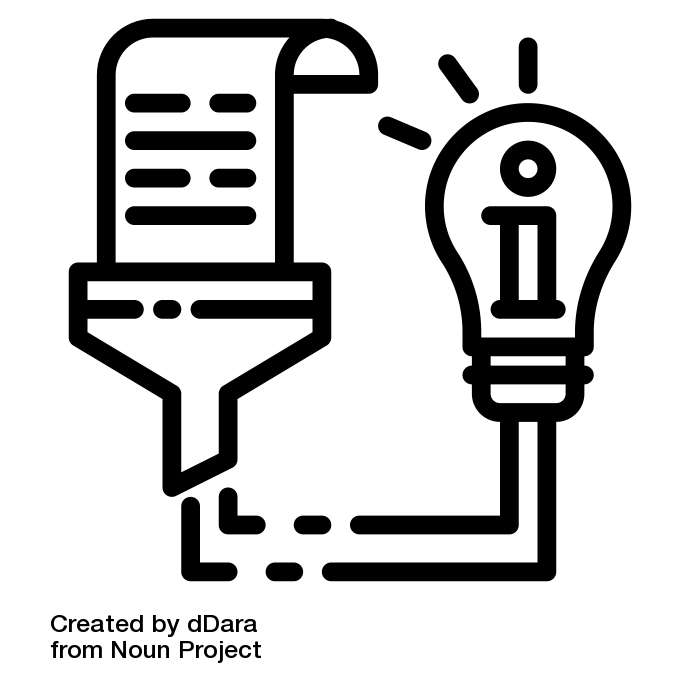
\includegraphics[width=0.9\textwidth]{symbols/symbol_tex_content}
				\end{wrapfigure}
				
				In diesen Texten findest du Erklärungen und Hintergründe! \newline 
				Die Quellen findest du in den Fußnoten. Diese Quellen können dir auch als Quizvorbereitung helfen. Übrigens, nicht alle Quellen sind Wikipedia. Aber es ist eine nützliche – und in Chemie akzeptierte Quelle. 
				\vspace{0.7cm}  % to fill empty space in tcolorbox
			\end{tcolorbox}

			\begin{tcolorbox}[enhanced,
				colback=white,
				colframe=orange!60!red,
				fonttitle=\sffamily\bfseries\large, 
				title=Wiederholung,  % search keyword::Wiederholung
				attach boxed title to top left={xshift=3.2mm,yshift=-0.50mm},
				boxed title style={skin=enhancedfirst jigsaw,size=small,arc=1mm,bottom=-1mm,colframe=orange!60!red,height=0.75cm},
				colbacktitle=orange!60!red,
				% sharp corners,
				drop lifted shadow]	
				\begin{wrapfigure}{L}{0.15\textwidth}  
					\centering
					\vspace{-14pt}  % to align image with first line of text
					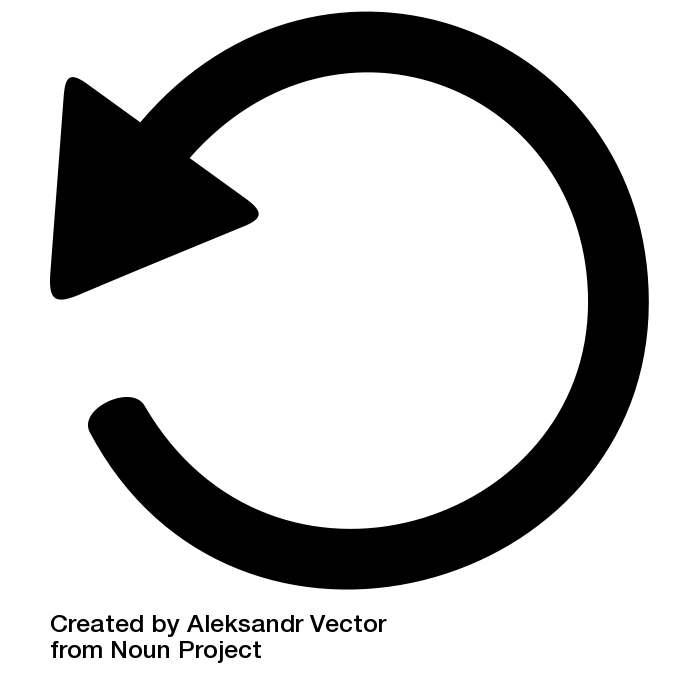
\includegraphics[width=0.9\textwidth]{symbols/symbol_tex_review}
				\end{wrapfigure}
				
				An diesen Stellen sollst du dein Wissen auffrischen! \newline 
				Du solltest die entsprechenden Themen schon vorher im (Chemie-)Unterricht behandelt haben. Falls nicht, arbeite deine Wissenslücken bitte selbstständig auf. 
				\vspace{1.0cm}
			\end{tcolorbox}
			
			
			\begin{tcolorbox}[enhanced,
				colback=white,
				colframe=black,
				fonttitle=\sffamily\bfseries\large, 
				title=Internet-Quelle (URL),  % search keyword::URL
				attach boxed title to top left={xshift=3.2mm,yshift=-0.50mm},
				boxed title style={skin=enhancedfirst jigsaw,size=small,arc=1mm,bottom=-1mm,colframe=black,height=0.75cm},
				colbacktitle=black,
				drop lifted shadow]
				\begin{wrapfigure}{L}{0.15\textwidth}  
					\centering
					\vspace{-14pt}  % to align image with first line of text
					
\includegraphics[width=0.9\textwidth]{symbols/symbol_tex_qrcode}
				\end{wrapfigure}
				
				Manche Online-Quellen haben nicht ins Skript gepasst. Daher kannst du mit einem Handy diese QR-Codes einlesen und so die Weblinks (URLs) öffnen. 
				\vspace{1.5cm}  % to fill empty space in tcolorbox
			\end{tcolorbox}
			
			\begin{tcolorbox}[enhanced,
				colback=white,
				colframe=green!30!black,
				fonttitle=\sffamily\bfseries\large, 
				title=Durchführung,  % search keyword::Durchführung
				attach boxed title to top left={xshift=3.2mm,yshift=-0.50mm},
				boxed title style={skin=enhancedfirst jigsaw,size=small,arc=1mm,bottom=-1mm,colframe=green!50!black,height=0.75cm},
				colbacktitle=green!50!black,
				drop lifted shadow]
				\begin{wrapfigure}{L}{0.15\textwidth}  
					\centering
					\vspace{-14pt}  % to align image with first line of text
					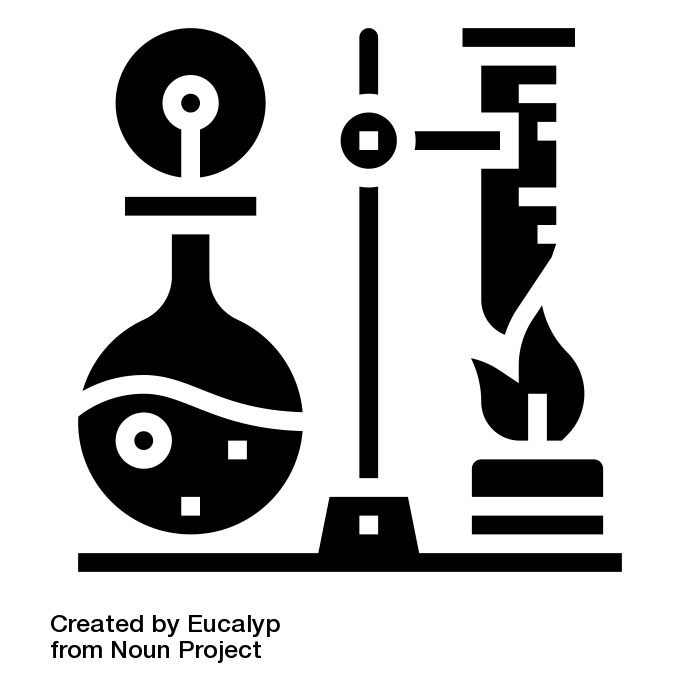
\includegraphics[width=0.9\textwidth]{symbols/symbol_tex_method}
				\end{wrapfigure}
				
				Dieses Symbol weißt immer auf eine Durchführung für ein Experiment hin. 
				\vspace{2.3cm}  % to fill empty space in tcolorbox
			\end{tcolorbox}
			
			\begin{tcolorbox}[enhanced,
				colback=white,
				colframe=red,
				fonttitle=\sffamily\bfseries\large, 
				title=Für schnelle Schüler\_innen,  % search keyword::schnelle_Schüler
				attach boxed title to top left={xshift=3.2mm,yshift=-0.40mm},
				boxed title style={skin=enhancedfirst jigsaw,size=small,arc=1mm,bottom=-1mm,colframe=red,height=0.75cm},
				colbacktitle=red,
				drop lifted shadow]
				\begin{wrapfigure}{L}{0.15\textwidth}  
					\centering
					\vspace{-14pt}  % to align image with first line of text
					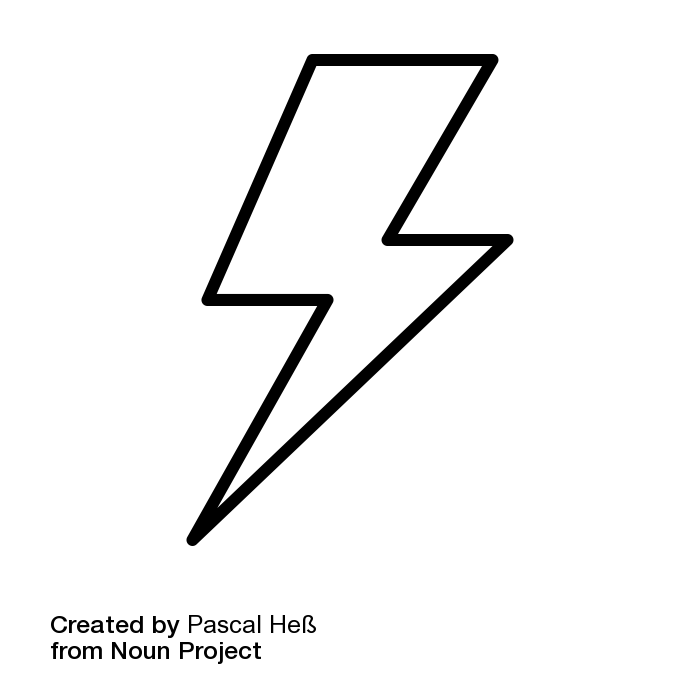
\includegraphics[width=0.8\textwidth]{symbols/symbol_tex_faststudents}
				\end{wrapfigure}
				
				Es soll keine Langeweile aufkommen. Wenn du mit Aufträgen bereits fertig bist, während deine Gruppe noch arbeitet, kannst du dich hier noch weiter in das Thema vertiefen. 
				\vspace{1.2cm}  % to fill empty space in tcolorbox
			\end{tcolorbox}
			
			\begin{tcolorbox}
				[enhanced,
				colback=white,
				colframe=black,
				fonttitle=\sffamily\bfseries\large, 
				title=Zeit,  % search keyword::Zeit
				attach boxed title to top left={xshift=3.2mm,yshift=-0.40mm},
				boxed title style={skin=enhancedfirst
					jigsaw,size=small,arc=1mm,bottom=-1mm,colframe=black,height=0.75cm},
				colbacktitle=black,
				drop lifted shadow]
				\begin{wrapfigure}{L}{0.15\textwidth}
					\centering
					\vspace{-14pt}  % to align image with first line of text
					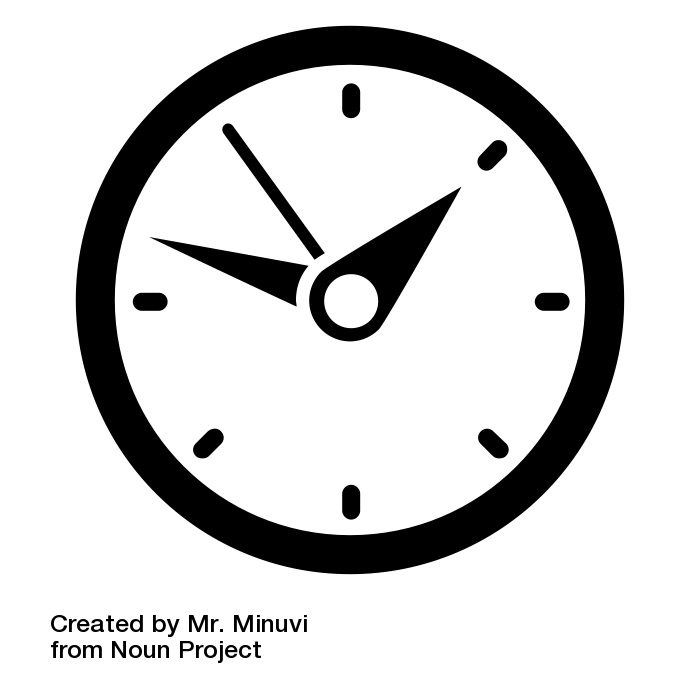
\includegraphics[width=0.7\textwidth]{symbols/symbol_tex_time}
				\end{wrapfigure}
				
				Das Zeitsymbol soll dir zeigen, wie lange du für das jeweilige Kapitel brauchen solltest. Diese Zeitangabe dient aber nur als Orientierung. Am Ende musst du nur die Planung deiner Lehrkraft und deine eigene Zeitplanung beachten. 
				\vspace{1.0cm}  % to fill empty space in tcolorbox
			\end{tcolorbox}
			
% *******************************************
% Template for box "without" specific purpose
% *******************************************
% this is sometimes used for dialogues or chat-entries as context for tasks
			
%{\fontfamily{qag}\selectfont  % set different font for chat-entry
%			\begin{tcolorbox}[enhanced,
%				colback=white,
%				colframe=teal,
%				fonttitle=\sffamily\bfseries\large, 
%				title=Alexanders Logbuch, 
%				attach boxed title to top left={xshift=3.2mm,yshift=-0.50mm},
%				boxed title style={skin=enhancedfirst jigsaw,size=small,arc=1mm,bottom=-1mm,colframe=teal,height=0.6cm},
%				colbacktitle=teal,
%				drop lifted shadow]
%				
%				
%				
%				Danke für die Hilfe, aber es scheint noch etwas schwieriger zu sein. Die Maschine zeigt eine Fehlermeldung: das Gesetz der Erhaltung der Masse muss beachtet werden. Wir sollen die Formelgleichung \textit{ausgleichen}. Was heißt das? Wo ist der Professor, wenn man ihn braucht?!
%				% \vspace{1.3cm}  % to fill empty space in tcolorbox
%			\end{tcolorbox}
%}  % end different font for chat entry

				
				
		\subsection*{Bewertung}
			
			Das Thema Biolpolymere wird uns das ganze Semester beschäftigen. In dieser Zeit müssen Sie folgende Leistungen erbringen:
			
			\begin{enumerate}
				\item \textbf{Ausführliche Protokolle}
				\item Zwei \textbf{Tests}
				\item \textbf{Klausur oder Stundenarbeit zur Klausur}
				\item \textbf{Portfolio}
				\item (Mündliche) \textbf{Mitarbeit} in Plenumsphasen.
			\end{enumerate}
						
			\subsubsection*{Das Portfolio}
			
				Das Portfolio ist ein Teil der Arbeit und Bewertung. Zum einen dient es der Sicherung und Sammlung aller Arbeitsergebnisse. Sie können und sollten in diesem Portfolio alles sammeln, was Sie an Materialien und Produkten selbst erarbeitetet haben. 
				Die zweite Funktion des Portfolios ist die Darstellung Ihrer eigenen Entwicklung. Mit Hilfe des Portfolios belegen Sie Ihren Lernfortschritt und reflektieren Ihre Arbeitsergebnisse und  Arbeitsweisen. Diese Reflexion sollte sich  auf alle Arbeitsprozesse, wie z.B. Recherchen oder Gruppenarbeiten, beziehen. Die Selbstreflexion sollte unabhängig von den Arbeitsaufträgen der Lehrkraft erfolgen. \newline
				Darüber hinaus können Sie dieses Portfolio auch als Teil Ihrer zukünftigen Bewerbungsmappen nutzen. Ihr zukünftiger Arbeitgeber erlangt dadurch ein umfassenderes Bild von Ihnen. Sehen Sie das Portfolio also nicht nur als weiteren Schulhefter sondern auch als Selbstdarstellungsmöglichkeit. \newline
				Die Bewertung des Portfolios erfolgt zum Ende des jeweiligen Semesters und erfolgt mit Hilfe des gegebenen Bewertungsrasters.
						 
					
			\subsubsection*{Hilfreiche Fragen für die Reflexion}
					
				\begin{center}
					\smartdiagramset{
						planet size=3cm, 
						distance planet-text=0.1,
						distance planet-satellite=4.5cm,
						% /tikz/connection planet satellite/.append style={<-}
					} 
					\smartdiagram[constellation diagram]{Reflexion, {Habe ich die Zeit effektiv genutzt?}, {Habe ich alle Aufträge gelöst?}, {Habe ich alles verstanden?},  {Habe ich gut allein gearbeitet?}, {Habe ich gut in der Gruppe gearbeitet?}, {Was kann ich in der nächsten Stunde besser machen?}}
				\end{center}
				
				\noindent Für eine schnelle Reflexion kann man dieses Diagramm benutzen. Im Portfolio sollte dann aberzusätzlich eine ausführliche Reflexion in Textform zu finden sein. Am Ende jedes Kapitels findet man eine Kurzreflexion. Aber im Portfolio können Sie auch öfter reflektieren. 
				
				% ***** start copy here *********************************************************
				% *******************************************************************************
				%            __ _           _   _                        _                _   
				%  _ __ ___ / _| | ___  ___| |_(_) ___  _ __         ___| |__   __ _ _ __| |_ 
				% | '__/ _ \ |_| |/ _ \/ __| __| |/ _ \| '_ \ _____ / __| '_ \ / _` | '__| __|
				% | | |  __/  _| |  __/ (__| |_| | (_) | | | |_____| (__| | | | (_| | |  | |_ 
				% |_|  \___|_| |_|\___|\___|\__|_|\___/|_| |_|      \___|_| |_|\__,_|_|   \__|
				%                                                                            
				%
				
				\vspace{0.3cm}
				\begin{center}
					\begin{tcolorbox}[enhanced,
						width=0.75\textwidth,
						colback=white,
						colframe=darkgray,
						fonttitle=\sffamily\bfseries\large, 
						title=Kurzreflexion,  % search keyword::Informationstexte 
						attach boxed title to top left={xshift=3.2mm,yshift=-0.50mm},
						boxed title style={skin=enhancedfirst jigsaw,size=small,arc=1mm,bottom=-1mm,colframe=darkgray,height=0.75cm},
						colbacktitle=darkgray,
						drop lifted shadow]
						
						% \begin{figure}[htbp]  % not good in ecolorbox
						\textbf{Auftrag: Bewerten Sie Ihre Arbeit in der letzten Einheit selbst.} \newline
						\begin{center}
						\begin{tikzpicture}[scale=1]
							\path (0:0cm) coordinate (O); % define coordinate for origin
							
							% draw the spiderweb
							\foreach \X in {1,...,\D}{
								\draw (\X*\A:0) -- (\X*\A:\R);
							}
							
							\foreach \Y in {0,...,\U}{
								\foreach \X in {1,...,\D}{
							\path (\X*\A:\Y*\R/\U) coordinate (D\X-\Y);
							\fill (D\X-\Y) circle (1pt);
								}
								\draw [opacity=0.3] (0:\Y*\R/\U) \foreach \X in {1,...,\D}{
									-- (\X*\A:\Y*\R/\U)
								} -- cycle;
							}
							
							% define labels for each dimension axis (names config option)
							\path (1*\A:\L) node (L1) {\tiny Verständnis};
							\path (2*\A:\L) node (L2) {\tiny alle Aufgaben gelöst};
							\path (3*\A:\L) node (L3) {\tiny Zeit effektiv genutz};
							\path (4*\A:\L) node (L4) {\tiny Einzelarbeit};
							\path (5*\A:\L) node (L5) {\tiny Gruppenarbeit};
						
						\end{tikzpicture}
						% \caption{Diagramm Slebstreflexion}
						% \caption{Spiderweb Diagram (\D~Dimensions, \U-Notch Scale, 3 Samples)}
						% \label{fig:spiderweb}
						% \end{figure} 
						\end{center}
						\textbf{{\Large Was können Sie in der nächsten Stunde verbessern?}}
					
					\end{tcolorbox}
				\end{center}
				% *******************************************************************************
				% ***** end copy here ***********************************************************
						
					
\newpage
					
\begin{landscape}
						
			\subsubsection*{Bewertungsraster für das Portfolio}
				
				Die Bewertung des Portfolios erfolgt zum Ende des Halbjahres und mit Hilfe dieses Bewertungsrasters. \newline
						
				\begin{tabular}{|l|*{4}{p{4.5cm}|}}  % da alle Spalten gleich sein sollen: Sternoperator {*{Anzahl n}{Spaltentyp}}
					\hline
					% *** 1. Zeile **************************************************
					\textbf{Kriterium} &
					\textbf{1BE} &
					\textbf{2BE} &
					\textbf{3BE} &
					\textbf{4BE} \\
					\hline
					% *** 2. Zeile **************************************************
					\multicolumn{5}{c}{\textbf{Umsetzung Portfolio - Notenpunkte}} \\
					\hline
					% *** 3. Zeile **************************************************
					\textbf{Umsetzung} &
					einfaches HTML &
					schönes HTML &
					mit HTML und CSS einfach gestaltet &
					mit HTML und CSS (und JS) kreativ gestaltet \\
					\hline
					% *** 7. Zeile **************************************************
					\multicolumn{5}{c}{\textbf{Inhaltliche Kriterien (Gewichtung 2)}} \\
					\hline
					% *** 8. Zeile **************************************************
					\textbf{Dokumentation} &
					Weniger als zur Hälfte erfüllt &
					Mehr als zur Hälfte erfüllt &
					Weitgehend erfüllt &
					Vollständig erfüllt \\
					\hline
					% *** 9. Zeile **************************************************
					\multicolumn{5}{c}{\textbf{Reflexion der Arbeit und des Erkenntnisgewinns (Gewichtung 3)}} \\
					\hline
					% *** 10. Zeile **************************************************
					\textbf{Reflexion} &
					\textbf{Kaum Reflexionsfähigkeit erkennbar.} Die Kurzreflexionen wurden selten genutzt oder das Semester wurde abschließend reflektiert oder die Reflexion wurde während des Semsters manchmal vorgenommen. &
					\textbf{Reflexionsfähigkeit zum Teil erkennbar.} Die Kurzreflexionen wurden selten genutzt. Das Semester wurde abschließend reflektiert oder die Reflexion wurde während des Semsters manchmal vorgenommen. &
					\textbf{Gute Reflexionsfähigkeit erkennbar.} Die Reflexion wurde mehrfach während des Semsters vorgenommen. Die Kurzreflexionen wurden genutzt. Das Semester wurde abschließend ergänzend reflektiert.  &
					\textbf{Sehr gute Reflexionsfähigkeit erkennbar.} Die Reflexion wurde mehrfach während des Semsters vorgenommen. Die Kurzreflexionen wurden sinnvoll genutzt. Das Semester wurde abschließend ausführlich ergänzend und glaubhaft reflektiert. \\
					\hline
				\end{tabular} \newline
					
				\vspace{1cm}
				
				\noindent Die \textit{Dokumentation} der Arbeit enthält z.B. die Lösungen zu den Arbeitsaufträgen, weitere Mitschriften, Quellen, Recherchen, Bilder, Mind-Maps, Videos etc. \newline
				Die durchgängige \textit{Reflexion} beinhaltet die Arbeit im Kurs, in der Gruppe, Einzelarbeit, die Reflexion des Erkenntnisstands etc.
						
\end{landscape}
			
			%TODO: Text zur Bewertung und genauen Arbeitsweise einfügen!
			
\newpage
	\part{Der Bierbrauprozess}
	
	\section{Der Bierbrauprozess}

		\textit{Bierbrauen ist eine lebensmitteltechnischer Prozess, den die Menschheit schon seit Jahrtausenden überall auf der Welt praktiziert. Im Vergleich zur Weinherstellung benötigt man einige Arbeitsschritte mehr. Wie kann man also Bier herstellen? Benötigt man dazu immer eine große Brauerei? Kann man das auch in der Schule oder zu Hause machen?} \newline
		
		\begin{minipage}{0.7\textwidth}
			\noindent \textbf{Am Ende dieses Kapitels sollen Sie ... :}
			\begin{enumerate}
				\item ... den Ablauf des Bierbrauens beschreiben können.
				\item ... die Bedeutung der einzelnen Stationen erklären können.
				\item ... die genauen Vorgänge beim Maischen und die beteiligten Stoffe nennen können.
				\item ... die beteiligten Biopolymere und deren chemische Stoffgruppen nennen können.
				\item ... chemisch-technische Prozesse mit schematischen Darstellungen beschreiben können.
				\item ... Informationen mit Hilfe von Tabellen und Mind-Maps strukturieren können.
			\end{enumerate}
			\textbf{Vorgehensweise:}
			\begin{enumerate}
				\item Arbeiten Sie erst einmal allein.
				\item Nachdem Sie die Recherche erledigt haben, tauschen Sie sich mit einigen MitschülerInnen aus.
				\item Bearbeiten Sie dann den Rest der Aufgaben. 
			\end{enumerate}
			
		\end{minipage}
		\hspace{0.1\textwidth}
		\begin{minipage}{0.2\textwidth}
			\begin{tcolorbox}
				[enhanced,
				width=0.9\textwidth,
				colback=white,
				colframe=black,
				fonttitle=\sffamily\bfseries\large, 
				title=Zeit,  % search keyword::Zeit
				attach boxed title to top center={xshift=-0.0mm,yshift=-0.50mm},
				boxed title style={skin=enhancedfirst jigsaw,size=small,arc=1mm,bottom=-1mm,colframe=black,height=0.75cm},
				colbacktitle=black,
				drop lifted shadow]
				\centering
				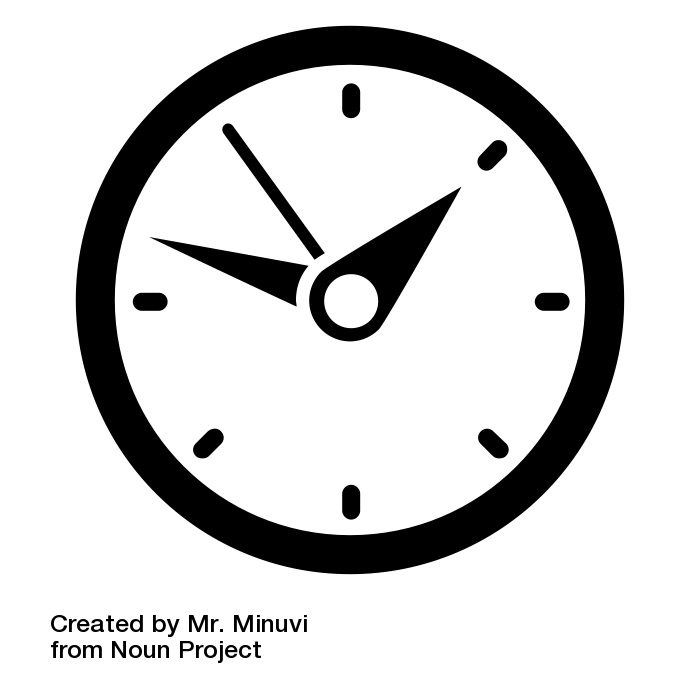
\includegraphics[width=0.9\textwidth]{symbols/symbol_tex_time}
				
				\begin{center}
					\textbf{90min}
				\end{center}
			\end{tcolorbox}
		\end{minipage}

\vspace{0.3cm}
		\begin{tcolorbox}[enhanced,
			colback=white,
			colframe=orange!60!red,
			fonttitle=\sffamily\bfseries\large, 
			title=Wiederholung,  % search keyword::Wiederholung
			attach boxed title to top left={xshift=3.2mm,yshift=-0.50mm},
			boxed title style={skin=enhancedfirst jigsaw,size=small,arc=1mm,bottom=-1mm,colframe=orange!60!red,height=0.75cm},
			colbacktitle=orange!60!red,
			% sharp corners,
			drop lifted shadow]	
			\begin{wrapfigure}{L}{0.15\textwidth}  
				\centering
				\vspace{-14pt}  % to align image with first line of text
				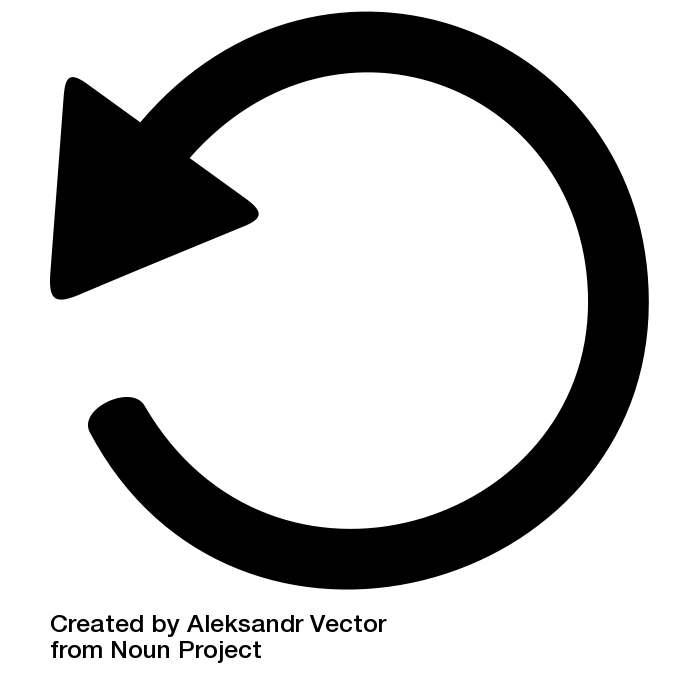
\includegraphics[width=0.9\textwidth]{symbols/symbol_tex_review}
			\end{wrapfigure}
			
			\textbf{Nennen Sie die allgemeinen Zutaten der alkoholischen Gärung. Beziehen Sie sich dabei auf die Weinherstellung.} \newline
			\textbf{Hören Sie sich den Soundtrack zum Skript an und lesen Sie die Lyrics. Nennen Sie die im Lied genannten Zutaten und Arbeitsschritte.}
			\begin{center}
				\includegraphics{images/qrcode_charliemops}
			\end{center}
			
		\end{tcolorbox}
		
		\begin{center}
			\noindent\rule{18cm}{0.1pt}
		\end{center}
			
\newpage
		\subsection{Ein Überblick zum Bierbrauprozess}
		
			\textbf{Auftrag: Beschreiben Sie den Prozess des Bierbrauens mit eigenen Worten!}
			\begin{enumerate}
				\item \textbf{Recherchieren} Sie, wie man Bier braut. Beginnen Sie mit dem Mälzen und Enden Sie beim Abfüllen.
				\item \textbf{Beschreiben} Sie den Prozess des Bierbrauen in einem Fließschema auf einem A3-Poster (Hefterportfolio) oder in Ihrem digitalen Portfolio. Nutzen Sie Bilder zur Beschreibung des Prozess.
			\end{enumerate}
			
			\begin{tcolorbox}[enhanced,
				colback=white,
				colframe=red,
				fonttitle=\sffamily\bfseries\large, 
				title=Für schnelle Schüler\_innen,  % search keyword::schnelle_Schüler
				attach boxed title to top left={xshift=3.2mm,yshift=-0.40mm},
				boxed title style={skin=enhancedfirst jigsaw,size=small,arc=1mm,bottom=-1mm,colframe=red,height=0.75cm},
				colbacktitle=red,
				drop lifted shadow]
				\begin{wrapfigure}{L}{0.15\textwidth}  
					\centering
					\vspace{-14pt}  % to align image with first line of text
					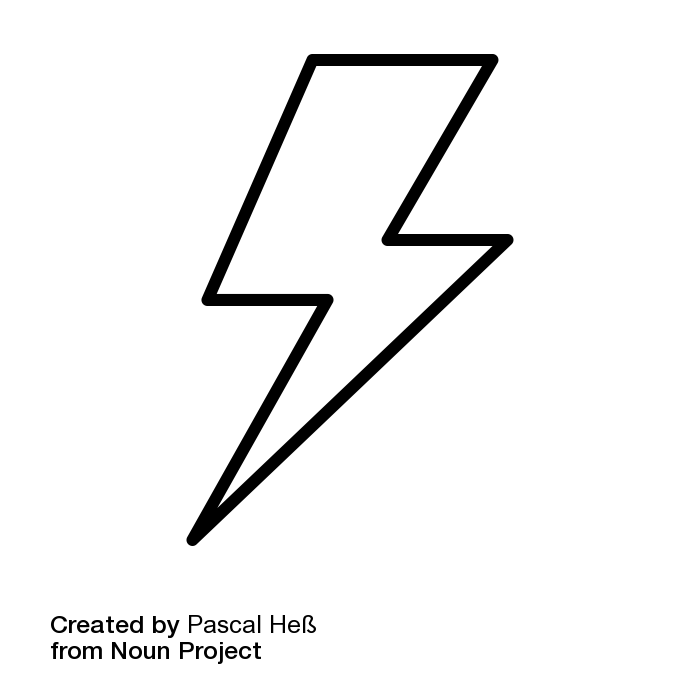
\includegraphics[width=0.8\textwidth]{symbols/symbol_tex_faststudents}
				\end{wrapfigure}
				
				Beim Bierbrauen wird oft von \textit{Hopfendolden} gesprochen. \textbf{Erklären} Sie den Begriff Dolden und \textbf{bewerten} Sie die Korrektheit dieses Begriffs.
				\vspace{1.2cm}  % to fill empty space in tcolorbox
			\end{tcolorbox}
				
		\subsection{Die Theorie des Maischens}
		
			\textit{Die Herstellung von Bier kann man aus verschiedenen Blickpunkten betrachten. Für die Chemiker ist vor allem der Maischevorgang am interessantesten, wenn es um Biopolymere geht.} \newline

			\noindent \textbf{Auftrag: Erstellen Sie eine tabellarische Übersicht zu den verschiedenen Stadien des	 Maischens.}
			\begin{enumerate}
				\item Recherchieren Sie, welche chemischen Prozesse genau beim Maischen ablaufen. Nutzen Sie dazu auch die gegebene Quelle.
				\item Übernehmen Sie die vorgegebene Tabelle in Ihrem Hefter und füllen Sie die entsprechenden Felder mit Hilfe der Informationen aus dem Text. Orientieren Sie sich dabei an den Temperaturen, bei denen die einzelnen Schritte stattfinden.
	% TODO: move this task to chapter 4.1 or 4.2
				\item Erstellen Sie eine Mind-Map zum Thema \textit{Biopolymere} beim Bierbrauen in Ihrem Portfolio.
			\end{enumerate}
			
			\begin{center}
				\begin{tabular}{|c|c|c|}
					\hline
					T in °C & Stufe/Rast und Bedeutung & Beteiligte Stoffe \\
					\hline
					... & ... & ... \\
					\hline
				\end{tabular}
			\end{center}
			
\vspace{0.3cm}
			\begin{tcolorbox}[enhanced,
				colback=white,
				colframe=black,
				fonttitle=\sffamily\bfseries\large, 
				title=Informationen zum Maischen,  % search keyword::URL
				attach boxed title to top left={xshift=3.2mm,yshift=-0.50mm},
				boxed title style={skin=enhancedfirst jigsaw,size=small,arc=1mm,bottom=-1mm,colframe=black,height=0.75cm},
				colbacktitle=black,
				drop lifted shadow]
				\begin{wrapfigure}{L}{0.15\textwidth}  
					\centering
					\vspace{-14pt}  % to align image with first line of text
					\includegraphics[width=0.9\textwidth]{images/qrecode_maischen_wiki}
				\end{wrapfigure}
				
					Hier finden Sie einige Informationen zu den Stadien des Maischens!!\footnote{Wenn Sie den QR-Code nicht scannen können, können Sie auch direkt aus der PDF-Datei auf die URL klicken}. \newline
					\textbf{Quelle} [Stand:12.8.2020]: \newline 
					\url{https://de.wikipedia.org/wiki/Bierbrauen#Maischen}
				\vspace{1.0cm}  % to fill empty space in tcolorbox
			\end{tcolorbox}

\vspace{0.3cm}
			\begin{tcolorbox}[enhanced,
				colback=white,
				colframe=black,
				fonttitle=\sffamily\bfseries\large, 
				title=Informationen zu den Rasten,  % search keyword::URL
				attach boxed title to top left={xshift=3.2mm,yshift=-0.50mm},
				boxed title style={skin=enhancedfirst jigsaw,size=small,arc=1mm,bottom=-1mm,colframe=black,height=0.75cm},
				colbacktitle=black,
				drop lifted shadow]
				\begin{wrapfigure}{L}{0.15\textwidth}  
					\centering
					\vspace{-14pt}  % to align image with first line of text
					\includegraphics[width=0.9\textwidth]{images/qrcode_rasten}
				\end{wrapfigure}
				
					Hier finden Sie einige Informationen zu den Stadien des Maischens! Achtung, die Begriffe sind alphabetisch geordnet. \footnote{Wenn Sie den QR-Code nicht scannen können, können Sie auch direkt aus der PDF-Datei auf die URL klicken}. \newline
					\textbf{Quelle} [Stand:12.8.2020]: \newline 
					\url{http://hobbybrauer-kompendium.de/r/rasten/rasten.html}
				\vspace{0.3cm}  % to fill empty space in tcolorbox
			\end{tcolorbox}
% TODO: weitere Quellen zu den Rasten einfügen

\newpage

				
				% ***** start copy here *********************************************************
				% *******************************************************************************
				%            __ _           _   _                        _                _   
				%  _ __ ___ / _| | ___  ___| |_(_) ___  _ __         ___| |__   __ _ _ __| |_ 
				% | '__/ _ \ |_| |/ _ \/ __| __| |/ _ \| '_ \ _____ / __| '_ \ / _` | '__| __|
				% | | |  __/  _| |  __/ (__| |_| | (_) | | | |_____| (__| | | | (_| | |  | |_ 
				% |_|  \___|_| |_|\___|\___|\__|_|\___/|_| |_|      \___|_| |_|\__,_|_|   \__|
				%                                                                            
				%
				
				\vspace{0.3cm}
				\begin{center}
					\begin{tcolorbox}[enhanced,
						width=0.75\textwidth,
						colback=white,
						colframe=darkgray,
						fonttitle=\sffamily\bfseries\large, 
						title=Kurzreflexion,  % search keyword::Informationstexte 
						attach boxed title to top left={xshift=3.2mm,yshift=-0.50mm},
						boxed title style={skin=enhancedfirst jigsaw,size=small,arc=1mm,bottom=-1mm,colframe=darkgray,height=0.75cm},
						colbacktitle=darkgray,
						drop lifted shadow]
						
						% \begin{figure}[htbp]  % not good in ecolorbox
						\textbf{Auftrag: Bewerten Sie Ihre Arbeit in der letzten Einheit selbst.} \newline
						\begin{center}
							\begin{tikzpicture}[scale=1]
								\path (0:0cm) coordinate (O); % define coordinate for origin
								
								% draw the spiderweb
								\foreach \X in {1,...,\D}{
									\draw (\X*\A:0) -- (\X*\A:\R);
								}
								
								\foreach \Y in {0,...,\U}{
									\foreach \X in {1,...,\D}{
								\path (\X*\A:\Y*\R/\U) coordinate (D\X-\Y);
								\fill (D\X-\Y) circle (1pt);
									}
									\draw [opacity=0.3] (0:\Y*\R/\U) \foreach \X in {1,...,\D}{
										-- (\X*\A:\Y*\R/\U)
									} -- cycle;
								}
								
								% define labels for each dimension axis (names config option)
								\path (1*\A:\L) node (L1) {\tiny Verständnis};
								\path (2*\A:\L) node (L2) {\tiny alle Aufgaben gelöst};
								\path (3*\A:\L) node (L3) {\tiny Zeit effektiv genutz};
								\path (4*\A:\L) node (L4) {\tiny Einzelarbeit};
								\path (5*\A:\L) node (L5) {\tiny Gruppenarbeit};
							
							\end{tikzpicture}
							% \caption{Diagramm Slebstreflexion}
							% \caption{Spiderweb Diagram (\D~Dimensions, \U-Notch Scale, 3 Samples)}
							% \label{fig:spiderweb}
							% \end{figure} 
						\end{center}
						\textbf{{\Large Was können Sie in der nächsten Stunde verbessern?}}
						\begin{center}
							%\vspace{1.1cm}
							\noindent\rule{12cm}{0.2pt}
							\vspace{1.1cm}
							\noindent\rule{12cm}{0.1pt}
							\vspace{1.1cm}
							\noindent\rule{12cm}{0.1pt}
							\vspace{1.1cm}
							\noindent\rule{12cm}{0.1pt}
							\vspace{1.1cm}
							\noindent\rule{12cm}{0.1pt}
							\vspace{1.1cm}
							\noindent\rule{12cm}{0.1pt}
							\vspace{1.1cm}
							\noindent\rule{12cm}{0.1pt}
							\vspace{1.1cm}
							\noindent\rule{12cm}{0.1pt}
						\end{center}
					\end{tcolorbox}
				\end{center}
								
				% *******************************************************************************
				% ***** end copy here ***********************************************************

\newpage
			
	\part{Die Chemie des Maischens}
	
	\section{Die Einteilung der Saccharide}
	
		\textit{Beim Maischen geht es hauptsächlich darum die Stärkemoleküle, die im Malz vorhanden sind zu zerkleinern und in gärfähige Zucker umzuwandeln. Aber was sind eigentlich Zucker? Was ist Stärke und Maltose und wie hängen diese Stoffe zusammen?
		Saccharide oder Kohlenhydrate werden oft bedeutungsgleich zu dem Begriff Zucker verwendet. Doch Kohlenhydrate sind eigentlich langkettige Moleküle, die aus vielen kleinen, spezifischen Bausteinen bestehen. Diese Bausteine werden in der Chemie als Zucker bezeichnet. Allerdings sind diese Zucker nicht mit dem Haushaltszucker zu verwechseln. Die Größe der Bausteine oder die länge der Kette wird als Einteilungsmerkmal genutzt.} \newline
		
		\begin{minipage}{0.7\textwidth}
			\noindent \textbf{Am Ende dieses Kapitels sollen Sie ... :}
			\begin{enumerate}
				\item ... die Einteilung der Saccharide erklären und übersichtlich darstellen können.

			\end{enumerate}
			\textbf{Vorgehensweise:}
			\begin{enumerate}
				\item Arbeiten Sie erst einmal allein.
				\item  Lesen Sie den Text und bearbeiten Sie die Arbeitsaufträge.
				\item  Vergleichen Sie ihre Ergebnisse mit Ihren MitschülerInnen.
				\item  Erweitern Sie die Mind-Maps aus den ersten Kapiteln.
			\end{enumerate}
			
		\end{minipage}
		\hspace{0.1\textwidth}
		\begin{minipage}{0.2\textwidth}
			\begin{tcolorbox}
				[enhanced,
				width=0.9\textwidth,
				colback=white,
				colframe=black,
				fonttitle=\sffamily\bfseries\large, 
				title=Zeit,  % search keyword::Zeit
				attach boxed title to top center={xshift=-0.0mm,yshift=-0.50mm},
				boxed title style={skin=enhancedfirst jigsaw,size=small,arc=1mm,bottom=-1mm,colframe=black,height=0.75cm},
				colbacktitle=black,
				drop lifted shadow]
				\centering
				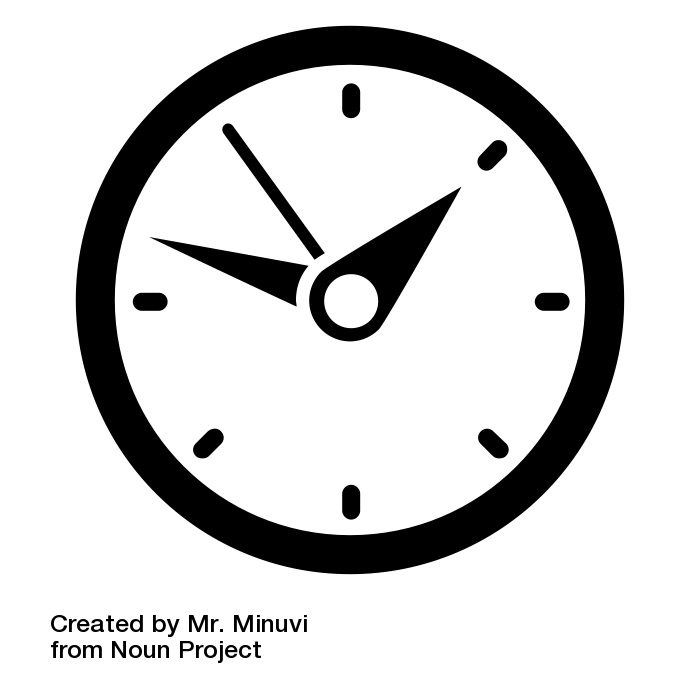
\includegraphics[width=0.9\textwidth]{symbols/symbol_tex_time}
				
				\begin{center}
					\textbf{90min}
				\end{center}
			\end{tcolorbox}
		\end{minipage}
		
		\begin{center}
			\noindent\rule{18cm}{0.1pt}
		\end{center}
	
\newpage		
		\subsection{Die Saccharide}
		
			\textbf{Auftrag: Erarbeiten Sie sich am Text einen Überblick zum Thema Saccharide!}
			\begin{enumerate}
				\item \textbf{Erstellen} Sie einen kurzen geschichtlichen Abriss zum Zucker (Tipp: Zeitstrahl)
				\item \textbf{Erstellen} Sie sich eine graphische Übersicht zu den Zuckern bzw. Sacchariden! Erweitern Sie dazu ihre Mind-Map aus den vorherigen Kapiteln.
			\end{enumerate}
			
			\begin{tcolorbox}[enhanced,
				colback=white,
				colframe=darkgray,
				fonttitle=\sffamily\bfseries\large, 
				title=Die Zucker,  % search keyword::Informationstexte 
				attach boxed title to top left={xshift=3.2mm,yshift=-0.50mm},
				boxed title style={skin=enhancedfirst jigsaw,size=small,arc=1mm,bottom=-1mm,colframe=darkgray,height=0.75cm},
				colbacktitle=darkgray,
				drop lifted shadow]
				\begin{wrapfigure}{L}{0.15\textwidth}  
					\centering
					\vspace{-14pt}  % to align image with first line of text
					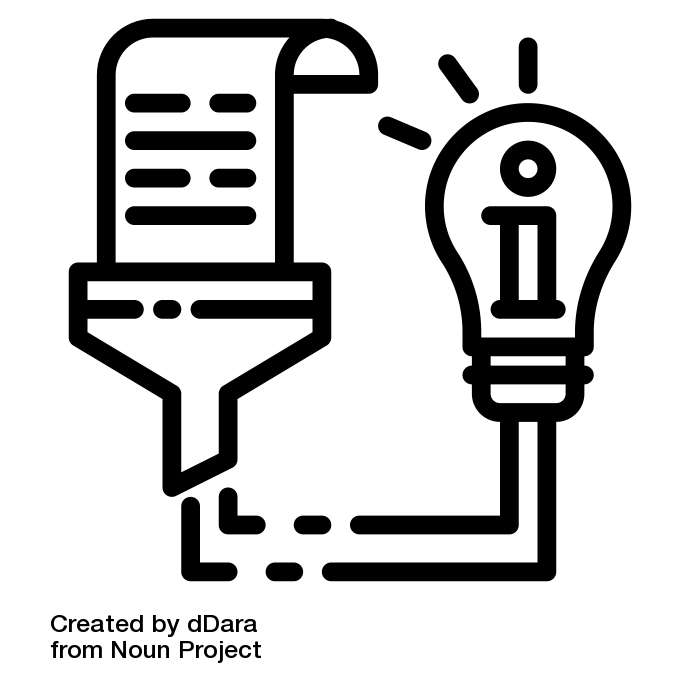
\includegraphics[width=0.9\textwidth]{symbols/symbol_tex_content}
				\end{wrapfigure}
				
				Zucker wurde bereits um 700 v. Chr. in China und Indien aus Zuckerrohr gewonnen. Dieses stammt ursprünglich aus Polynesien. Über Persien und Ägypten verbreitete sich der Zuckerrohranbau Richtung Westen. Um 800 n.Chr. war Zucker bereits in allen wärmeren Gebieten rund um das Mittelmeer bekannt. 1319 gelange der erste Zucker nach England und war dort eine teure Neuheit, welche anfangs nur für medizinische Zwecke verwendet wurde. \newline
				Da Zucker importiert werden musste, blieb es bis zum 17.Jahrhundert ein reines Luxusgut. Erst dann kamen billige Importe von den karibischen Inseln nach Europa. Durch die Feldzüge Napoleons und die kriegerischen Auseinandersetzungen  wurde Frankreich von der Versorgung mit Zucker abgeschnitten. Napoleon beauftragte Wissenschaftler Alternativen zu suchen. Man griff auf Erkenntnisse von Andreas Marggraf zurück. Dieser entdeckte, dass Zucker auch aus Wurzelfrüchten, wie z.B. Pastinaken, extrahiert werden konnte. Man führte gezielte Züchtungsversuche durch und erschaffte nach 10 Jahren eine anbaureife Rübenart. Damit begann die europäische Zuckerrübenwirtschaft. Heute wird die Zuckerrübe in fast allen gemäßigten Zonen angebaut und übersteigt heute die Produktion von Rohrzucker.  \newline				
				Worum handelt es sich aber eigentlich um Zucker? Der Zucker aus dem Zuckerrohr und Zuckerrübe ist einfacher Haushaltszucker. Dieser ist ein Vertreter einer ganzen Gruppe chemischer verwandter Verbindungen, den Kohlenhydraten. Haushaltszucker wird chemisch als Saccharose oder Sucrose bezeichnet und besteht aus zwei Einfachzuckermolekülen. Saccharose ist ein Disaccharid.
				Die Einfachzucker, wie z.B. Glucose werden als Monosaccharide bezeichnet; langkettige Moleküle wie Stärke und Cellulose als Polysaccharide. Glucose ist das häufigste Monosaccharid und ist das Primärprodukt der Fotosynthese. Sie kommt in vielen Früchten und Gemüsen vor und ist die Hauptenergiequelle für Pflanzen und Tiere. Andere bekannte Monosaccharide sind Fructose (Fruchtzucker) und Galactose.  \newline
				Verbinden sich zwei Monosaccharide, entstehen, wie bereits erwähnt, Disaccharide. 
				Haushaltszucker ist z.B. eine Kombination aus Glucose und Fructose. Malzzucker (Maltose) hingegen besteht aus zwei Glucosemolekülen und Milchzucker (Lactose) ist aus Glucose und Galactose zusammengesetzt.  \newline
				Zucker die aus 3 bis 10 Monosacchariden bestehen, bezeichnet man als Oligosaccharide.
				Betrachtet man jedoch die produzierte Masse, stellen Polysaccharide die häufigsten Kohlenhydrate im Pflanzenreich dar, nämlich in Form von Stärke und Cellulose. Beide bestehen aus vielen aneinandergeknüpften Glucosemolekülen. Es gibt nur einen kleinen Unterschied in der Verknüpfung, doch dies hat eine große Folge. Während Stärke der Hauptlieferant menschlicher Nahrung ist, kann Cellulose nicht verdaut (oxidiert) werden und passiert unverändert unseren Verdauungstrakt. Solche Nahrungsstoffe werden als Ballaststoffe bezeichnet. Sie liefern zwar keine Energie, fördern aber unser Wohlbefinden. \footnote{Emsley, John; Kellersohn, Thomas. Parfüm, Portwein, PVC… .Wiley-VCH Verlag GmbH \& Co. KGaA; 1. Aufl. 2003}
			\end{tcolorbox}
		
\vspace{0.3cm}			
			\begin{tcolorbox}[enhanced,
				colback=white,
				colframe=red,
				fonttitle=\sffamily\bfseries\large, 
				title=Für schnelle Schüler\_innen,  % search keyword::schnelle_Schüler
				attach boxed title to top left={xshift=3.2mm,yshift=-0.40mm},
				boxed title style={skin=enhancedfirst jigsaw,size=small,arc=1mm,bottom=-1mm,colframe=red,height=0.75cm},
				colbacktitle=red,
				drop lifted shadow]
				\begin{wrapfigure}{L}{0.15\textwidth}  
					\centering
					\vspace{-14pt}  % to align image with first line of text
					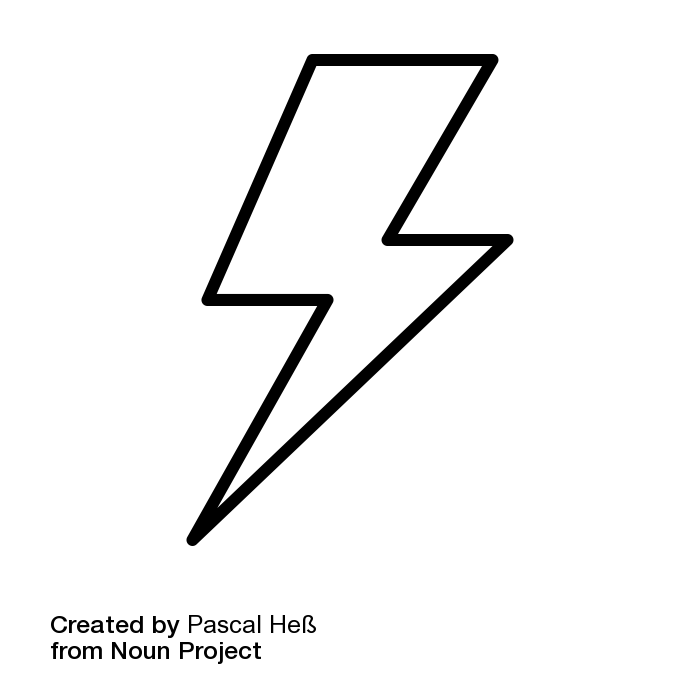
\includegraphics[width=0.8\textwidth]{symbols/symbol_tex_faststudents}
				\end{wrapfigure}
				
				\textbf{Recherchieren} Sie, warum (Haushalts)Zucker als Konservierungsmittel genutzt werden kann.
				\newline
				In einem Film wird behauptet, dass Zucker früher auch als \textit{Desinfektionsmittel} für Wunden genutzt wurde. \textbf{Recherchieren} Sie diesen Zusammenhang und \textbf{bewerten} Sie die Filmaussage.
				
			\end{tcolorbox}

\newpage
	% *************************************************
	% Anfang Kapitelübersicht // Begin Chapter Overview
	% *************************************************
	\section{Von der Stärke zur Maltose}
	
		\textit{Man kann die Zucker von zweiten Seiten aus aufarbeiten. Entweder man fängt bei den Monosacchairde, den kleinsten Bausteinen, an oder man schaut sich zuerst die Polymere, die langen Ketten, die durch die Monomerbausteine gebildet werden an. Stärke ist ein solches (Bio-)Polymer. 
		Um die Vorgänge beim Maischen richtig zu verstehen, kommt man nicht ohne eine Untersuchung der beteiligten Enzyme aus. } \newline
	
		\begin{minipage}{0.7\textwidth}
			% *******************************
			% Übersicht Lernziele // Overview  
			% *******************************
			\noindent \textbf{Am Ende dieses Kapitels sollen Sie ... :}
			\begin{enumerate}
				\item ... den Aufbau der Stärke beschreiben können.
				\item ... den Zusammenhang zwischen Enzymen, Proteinen und Bio-Polymeren erklären können.
				\item ... experimentell Stärke nachweisen können.
			\end{enumerate}
			% *************************************************
			% empfohlene Vorgehensweise // recommended approach  
			% *************************************************
			% Lernende können selbst entscheiden, wie sie sich durch das Kapitel arbeiten
			% Lehrpersonen/Lernende können folgende Empfehlung aber nutzen
			\textbf{Vorgehensweise:}
			\begin{enumerate}
				\item Arbeiten Sie erst einmal allein.
				\item Lesen Sie den Text und bearbeiten Sie den Arbeitsaufträge.
				\item Vergleichen Sie mit Ihren Mitschülern.
				\item Erweitern Sie die Mind-Maps aus den ersten Kapiteln. 
			\end{enumerate}
			
		\end{minipage}
		\hspace{0.1\textwidth}
		% ***********************************
		% empfohlene Zeit // recommended time  
		% ***********************************
		% zeitliche Orientierung für Lernende und Lehrpersonen
		% Zeit sollte aber ungefährt eingehalten werden, damit Reihenplanung funktioniert
		\begin{minipage}{0.2\textwidth}
			\begin{tcolorbox}
				[enhanced,
				width=0.9\textwidth,
				colback=white,
				colframe=black,
				fonttitle=\sffamily\bfseries\large, 
				title=Zeit,  % search keyword::Zeit
				attach boxed title to top center={xshift=-0.0mm,yshift=-0.50mm},
				boxed title style={skin=enhancedfirst jigsaw,size=small,arc=1mm,bottom=-1mm,colframe=black,height=0.75cm},
				colbacktitle=black,
				drop lifted shadow]
				\centering
				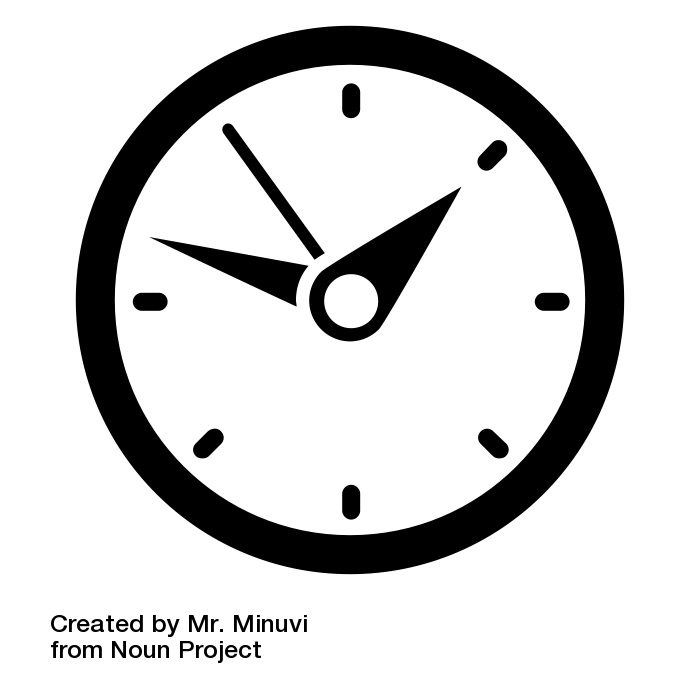
\includegraphics[width=0.9\textwidth]{symbols/symbol_tex_time}
				
				\begin{center}
					\textbf{135min} % Zeitangabe für Lernende // study time for students 
				\end{center}
			\end{tcolorbox}
		\end{minipage}

\vspace{0.3cm}
		% *********************************************
		% empfohlene Wiederholung // recommended review  
		% *********************************************
		\begin{tcolorbox}[enhanced,
			colback=white,
			colframe=orange!60!red,
			fonttitle=\sffamily\bfseries\large, 
			title=Wiederholung,  % search keyword::Wiederholung
			attach boxed title to top left={xshift=3.2mm,yshift=-0.50mm},
			boxed title style={skin=enhancedfirst jigsaw,size=small,arc=1mm,bottom=-1mm,colframe=orange!60!red,height=0.75cm},
			colbacktitle=orange!60!red,
			% sharp corners,
			drop lifted shadow]	
			\begin{wrapfigure}{L}{0.15\textwidth}  
				\centering
				\vspace{-14pt}  % to align image with first line of text
				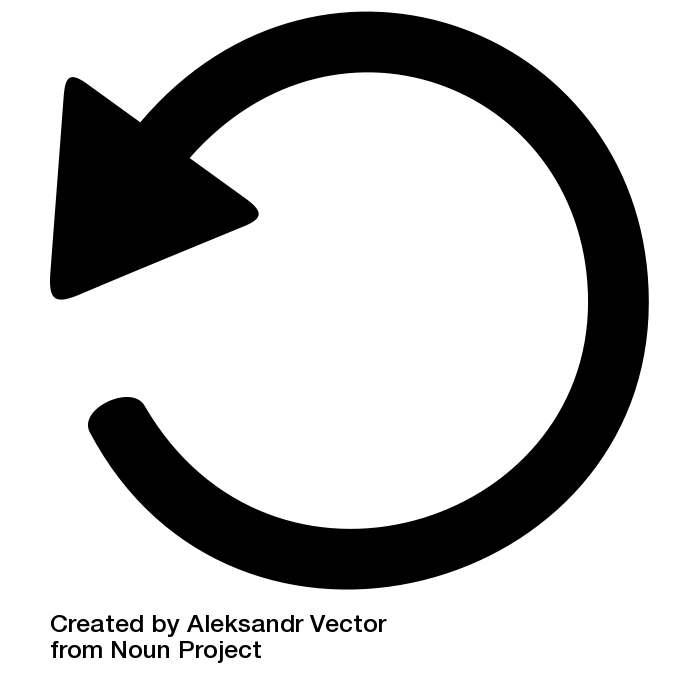
\includegraphics[width=0.9\textwidth]{symbols/symbol_tex_review}
			\end{wrapfigure}
			
			\textbf{Nennen Sie die drei Eigenschaften, die einen chemischen Katalysator auszeichnen.}
			\vspace{1.3cm}
			
		\end{tcolorbox}
		% Layout: Linie zum Abgrenzen
		\begin{center}
			\noindent\rule{18cm}{0.1pt}
		\end{center}
	% *********************************************
	% Ende Kapitelübersicht // End Chapter Overview
	% *********************************************				
\newpage
		
		\subsection{Der Aufbau der Stärke}
		
			\textbf{Auftrag: Erläutern Sie den Aufbau von Stärke.} \newline
			
			\begin{tcolorbox}[enhanced,
				colback=white,
				colframe=darkgray,
				fonttitle=\sffamily\bfseries\large, 
				title=Die Stärke,  % search keyword::Informationstexte 
				attach boxed title to top left={xshift=3.2mm,yshift=-0.50mm},
				boxed title style={skin=enhancedfirst jigsaw,size=small,arc=1mm,bottom=-1mm,colframe=darkgray,height=0.75cm},
				colbacktitle=darkgray,
				drop lifted shadow]
				\begin{wrapfigure}{L}{0.15\textwidth}  
					\centering
					\vspace{-14pt}  % to align image with first line of text
					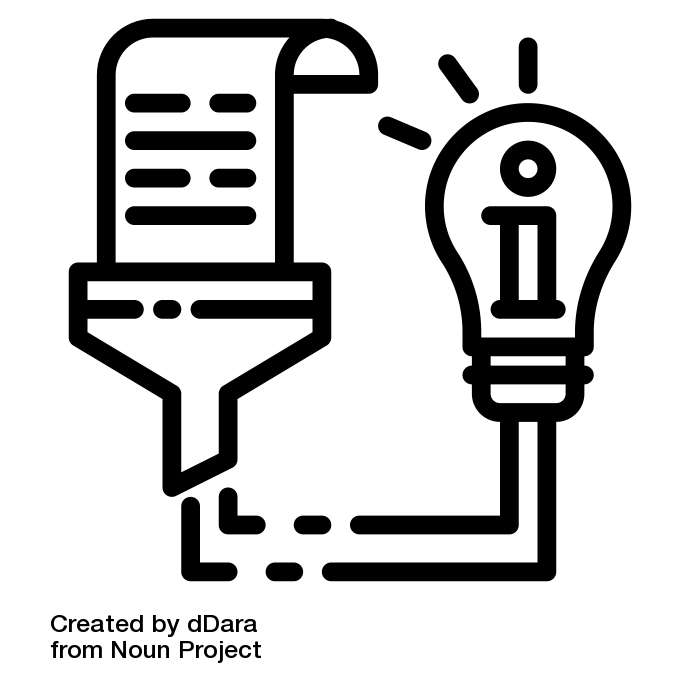
\includegraphics[width=0.9\textwidth]{symbols/symbol_tex_content}
				\end{wrapfigure}
				
				Stärkemoleküle bestehen aus bestimmten Glucose-Bausteinen, den D-Glucose-Einheiten, die über glykosidische Bindungen miteinander verknüpft sind. Dabei unterscheidet man, je nach Bindungstyp, zwei „Stärke-Typen“. 
				Stärke besteht meist zu 20–30\% aus Amylose. Amylose besteht aus Glucose-Monomeren, die linearen Ketten bilden. Die Glucose-Bausteine sind über Sauerstoffatome miteinander verbunden. Diese Ketten sind in einer Helixstruktur angeordnet. 
				Der zweite Stärke-Typ ist das Amylopektin. Es kommt 70-80\% in Stärke vor. Amylopektin bildet stark verzweigte Strukturen. 
				Die unterschiedlichen Strukturen entstehen durch verschiedene Bindungen, die die Glucose-Bausteine untereinander eingehen können. Allgemein wird dieser Bindungstyp als glykosidische Bindung bezeichnet. Wie verschiedene glykosidische Bindungen entstehen können, lernen Sie in einem späteren Kapitel.
				\begin{center}
					\includegraphics{images/staerke_aufbau}
				\end{center}
				Bei Zimmertemperatur können Wasser-Moleküle nicht durch die Hülle der Stärkekörner eindringen. Sie haften nur an der Oberfläche der Hülle. Beim Erwärmen beginnt das Amylopektin zu quellen, es nimmt dabei Wasser auf. Die Hülle wird so durchlässig, dass das Wasser zur Amylose gelangt und sich diese im Wasser löst.
				\footnote{Quelle Abbildung[Stand:12.8.2020]: https://www.seilnacht.com/Lexikon/kohlenh.html}
			\end{tcolorbox}
		
		\subsection{Enzyme und der Abbau der Stärke}
		
			\textbf{Auftrag: Helfen Sie IPAndi!}
			\begin{enumerate}
				\item \textbf{Lesen} Sie das Material zu Amylasen, Enzymen und Proteinen!
			    \item \textbf{Erklären} Sie, warum Amylase ein Bio-Polymer ist.
			    \item \textbf{Erläutern} Sie, wie zwei Aminosäuren über eine Peptidbindung verbunden werden können. \textbf{Erklären} Sie, warum es sich dabei um eine Kondensationsreaktion handelt.
			    \item \textbf{Erläutern} Sie, wie der Abbau der Stärke funktioniert.
			\end{enumerate}
			
{\fontfamily{qag}\selectfont  % set different font for chat-entry
			\begin{tcolorbox}[enhanced,
				colback=white,
				colframe=teal,
				fonttitle=\sffamily\bfseries\large, 
				title=Neulich im Bierbrauer-Forum, 
				attach boxed title to top left={xshift=3.2mm,yshift=-0.50mm},
				boxed title style={skin=enhancedfirst jigsaw,size=small,arc=1mm,bottom=-1mm,colframe=teal,height=0.6cm},
				colbacktitle=teal,
				drop lifted shadow]
				
				\textbf{{\Large IPAndi schrieb:}} \textit{Hallo Braugenossen, mein letztes Pils hat irgendwie zu süß geschmeckt. Und ich hatte das Gefühl, dass die Gärung auch nicht sehr lange lief. Der Alkoholgehalt kann also nicht so hoch gewesen sein. Was ist zu tun?} \newline
				\textbf{{\Large WeizenStefan schrieb:}} \textit{Kling schreibt dazu: „[...] Ein völliger Abbau (Umwandlung) der Kornstärke im Zucker durch die wiedererweckten Enzyme während der α- und β-Amylase des Maischvorgangs ist grundsätzlich anzustreben, um später einen optimalen Vergärungsgrad zu erreichen und um „pappig-süße“ Biere zu vermeiden. (Kling 2012: S81)1“ Schau dir auch die Iod-Probe an!} \footnote{Kling, Klaus. Bier selbst gebraut. Verlag Die Werkstatt. 3. Aufl. 2012. Göttingen.} \newline
				\textbf{{\Large IPAndi schrieb:}} \textit{Warum muss ich immer an die Oberchemiker/biologen geraten? Geht's auch auf Deutsch? Was hat den Kornstärke mit irgendwelchen Amylasen zu tun?}
			\end{tcolorbox}
}  % end different font for chat entry
		
			\begin{tcolorbox}[enhanced,
				colback=white,
				colframe=darkgray,
				fonttitle=\sffamily\bfseries\large, 
				title=Amylasen,  % search keyword::Informationstexte 
				attach boxed title to top left={xshift=3.2mm,yshift=-0.50mm},
				boxed title style={skin=enhancedfirst jigsaw,size=small,arc=1mm,bottom=-1mm,colframe=darkgray,height=0.75cm},
				colbacktitle=darkgray,
				drop lifted shadow]
				\begin{wrapfigure}{L}{0.15\textwidth}  
					\centering
					\vspace{-14pt}  % to align image with first line of text
					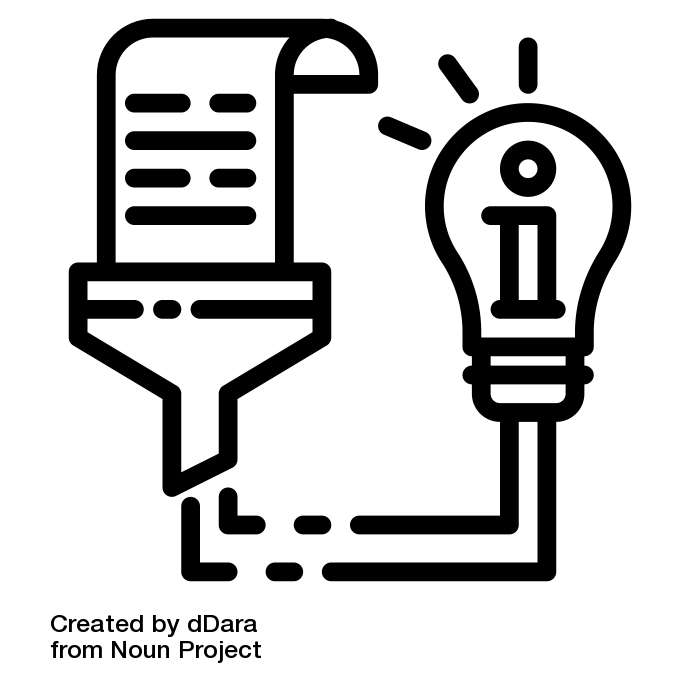
\includegraphics[width=0.9\textwidth]{symbols/symbol_tex_content}
				\end{wrapfigure}
				
				Amylasen sind Enzyme, die bei den meisten Lebewesen vorkommen und dort Polysaccharide abbauen. Ihre Wirkung besteht darin, dass sie Polysaccharide (z.B. Stärke) an den Glykosidbindungen spalten und abbauen. Amylase war das erste Enzym, das man entdeckte. Man unterscheidet zwei Typen:
				\begin{itemize}
					\item $\alpha$-Amylase spaltet nur die inneren Glykosidbindungen der Amylose. Dadurch entstehen Maltose, Maltotriose und verzweigte Oligosaccharide.
				    \item $\beta$-Amylase spaltet vom Kettenende her jeweils ein Maltosemolekül nach dem anderen ab. Sie kann daher umso besser wirken, je mehr Kettenenden durch die $\alpha$-Amylase bereits entstanden sind.
				\end{itemize}
				Beim Bierbrauen werden die natürlicherweise im Getreide vorkommenden Enzyme genutzt. Die Keimung wird angeregt und durch Darren abgebrochen (Mälzen). Im sogenannten Maischen werden in den Temperatur- und pH-Wert-Optima die Amylasen genutzt, um die Stärke des Getreides in vergärbare Einfach- und Zweifachzucker umzuwandeln.
				\footnote{Quelle abgewandelt: https://de.wikipedia.org/wiki/Amylasen [Stand: 22.8.2016]}
			\end{tcolorbox}

\vspace{0.3cm}
			\begin{tcolorbox}[enhanced,
				colback=white,
				colframe=darkgray,
				fonttitle=\sffamily\bfseries\large, 
				title=Enzyme,  % search keyword::Informationstexte 
				attach boxed title to top left={xshift=3.2mm,yshift=-0.50mm},
				boxed title style={skin=enhancedfirst jigsaw,size=small,arc=1mm,bottom=-1mm,colframe=darkgray,height=0.75cm},
				colbacktitle=darkgray,
				drop lifted shadow]
				\begin{wrapfigure}{L}{0.15\textwidth}  
					\centering
					\vspace{-14pt}  % to align image with first line of text
					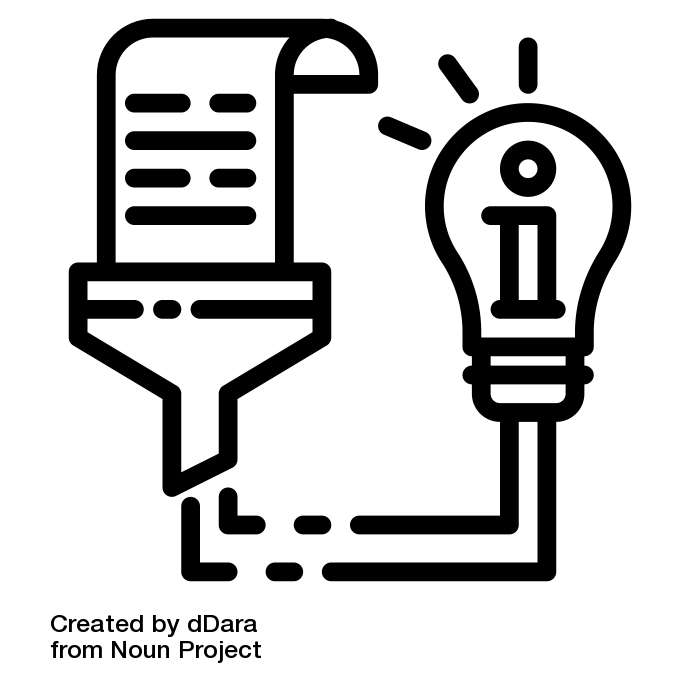
\includegraphics[width=0.9\textwidth]{symbols/symbol_tex_content}
				\end{wrapfigure}
				
				Enzyme sind Proteine mit katalytischen Eigenschaften. Man muss davon ausgehen, dass es kaum eine Proteinart gibt, die - wenn sie nicht als Stütz-, Transport-, Speichereiweiß oder als Antikörper dient - nicht die Funktion eines Enzyms hat. Die Anzahl der über zehntausend bis jetzt bekannten Enzyme weist darauf hin. 
				Die Enzyme unterscheiden sich von einfachen Proteinen (wie den Albuminen) durch das Vorhandensein eines oder mehrerer Zentren.
				\begin{itemize}
					\item Anlagerungszentren für Substrate und Cosubstrate,
				    \item Aktive Zentren, in denen die eigentliche Reaktion katalysiert wird,
				    \item Regulationszentren (zum Beispiel allosterische Zentren).
				\end{itemize}
				Die meisten Enzyme bestehen als Proteine nur aus kondensierten Aminosäuren; an der Katalyse sind deshalb nur deren Aminosäurereste beteiligt. Die Aminosäuren sind über Peptidbindungen miteinander verbunden.
				\footnote{Quelle abgewandelt: http://www.chemieunterricht.de/dc2/katalyse/k-enzym2.htm [Stand: 22.8.2016]}
			\end{tcolorbox}

\vspace{0.3cm}
			\begin{tcolorbox}[enhanced,
				colback=white,
				colframe=darkgray,
				fonttitle=\sffamily\bfseries\large, 
				title=Proteine,  % search keyword::Informationstexte 
				attach boxed title to top left={xshift=3.2mm,yshift=-0.50mm},
				boxed title style={skin=enhancedfirst jigsaw,size=small,arc=1mm,bottom=-1mm,colframe=darkgray,height=0.75cm},
				colbacktitle=darkgray,
				drop lifted shadow]
				\begin{wrapfigure}{L}{0.15\textwidth}  
					\centering
					\vspace{-14pt}  % to align image with first line of text
					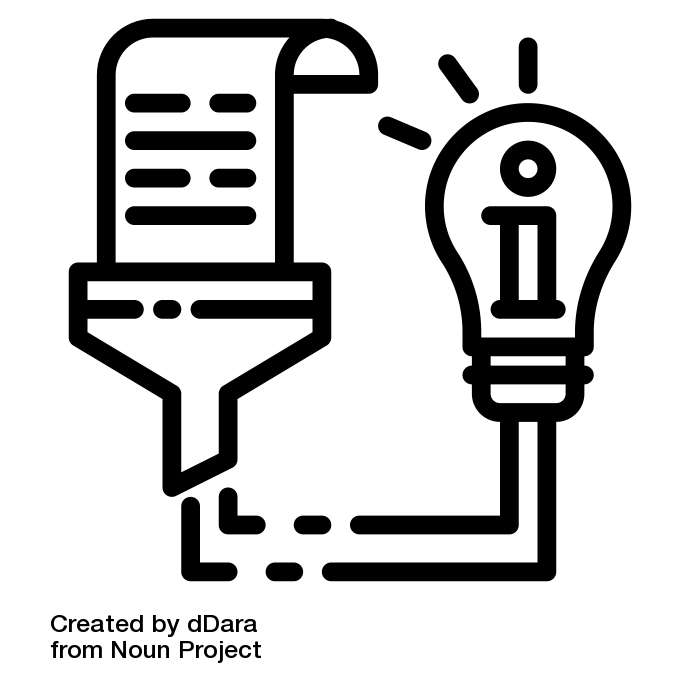
\includegraphics[width=0.9\textwidth]{symbols/symbol_tex_content}
				\end{wrapfigure}
				
				Proteine oder Eiweiße sind aus Aminosäuren aufgebaut. In der Natur gibt es wahrscheinlich mehrere hundert Aminosäuren, so konnte man sie sogar auf Kometen oder in Meteoriten nachweisen. Am Aufbau der Eiweiße im menschlichen Körper sind jedoch nur proteinogene Aminosäuren beteiligt. Aminosäuren enthalten sowohl die Carboxy-Gruppe \ch{COOH} als auch die Amino-Gruppe \ch{NH2}.
				\footnote{Quelle abgewandelt: http://www.seilnacht.com/Lexikon/amino.html [Stand: 22.8.2016]}
			\end{tcolorbox}

\vspace{0.3cm}
			\noindent \textbf{Auftrag: Weisen Sie Stärke in selbst gewählten Lebensmitteln nach!}
			\begin{enumerate}
				\item Führen Sie die Experimente durch und schreiben Sie ein \textbf{ausführliches Protokoll}!
			    \item Nutzen Sie die gegebenen Durchführungen.
			    \item \textbf{Erläutern} Sie in der Auswertung die chemischen Hintergründe der Beobachtungen und beantworten Sie \underline{auch} die gegebenen Fragen als Teil der Auswertung.
			    \item Besprechen Sie die Abgabefrist mit Ihrer Lehrkraft.
			\end{enumerate}	
			
			\begin{tcolorbox}[enhanced,
				colback=white,
				colframe=green!30!black,
				fonttitle=\sffamily\bfseries\large, 
				title=Durchführung,  % search keyword::Durchführung
				attach boxed title to top left={xshift=3.2mm,yshift=-0.50mm},
				boxed title style={skin=enhancedfirst jigsaw,size=small,arc=1mm,bottom=-1mm,colframe=green!50!black,height=0.75cm},
				colbacktitle=green!50!black,
				drop lifted shadow]
				\begin{wrapfigure}{L}{0.15\textwidth}  
					\centering
					\vspace{-14pt}  % to align image with first line of text
					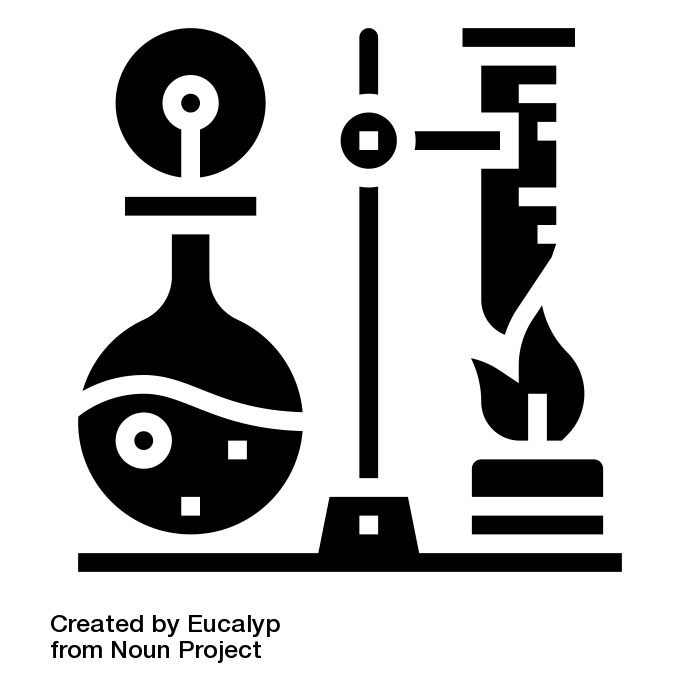
\includegraphics[width=0.9\textwidth]{symbols/symbol_tex_method}
				\end{wrapfigure}
				
				\textbf{1. Experiment: Nachweis von Stärke in Lebensmitteln} \newline
				Zum Nachweis von Stärke benutzt man die sog. Lugol’sche Lösung (Iod- Kaliumiodid-Lösung). Untersuchen Sie einige Lebensmitteln auf ihren Stärkegehalt, indem sie die einige Tropfen der Lugol’schen Lösung rauftropfen. 
				
				\textbf{2. Experiment: Temperaturabhängigkeit der Iod-Stärke-Reaktion} \newline
				a) Stärkekleister herstellen: Zu 1g Stärke wird so viel Wasser (einige Tropfen) gegeben, bis ein dicker Brei entsteht. Diesen gießt man in 100 ml nahezu siedendes Wasser. \newline
				b) Temperaturabhängigkeit testen: 1 ml Stärkekleister wird mit Wasser auf 100 ml verdünnt und mit einigen Tropfen Lugol’scher Lösung (Iod-Kaliumiodid-Lösung) versetzt. Nun wird abwechselnd erhitzt und wieder abgekühlt. \newline
				Tipp: ganz wenig Stärkekleister stark verdünnt und nur einen Tropfen Lugol’sche Lösung  
				
				\textbf{3. Experiment: Abbau von Stärke} \newline
				1 ml des Stärkekleisters aus Versuch 2 wird auf 100 ml verdünnt und mit einigen Tropfen Lugol’scher Lösung versetzt. Teilen Sie die Lösungen auf zwei Reagenzgläser auf und geben Sie zu einem Reagenzglas Spucke/Speichel hinzu. Warten Sie einige Minuten.
			\end{tcolorbox}	
			
\vspace{0.3cm}
			\noindent \textbf{Fragen für die Auswertung:}
			\begin{enumerate}
				\item \textbf{Erklären} Sie, warum die Iod-Stärke-Reaktion temperaturabhängig ist. Beziehen Sie sich dabei auf Ihre Kenntnisse zum chemischen Gleichgewicht.
				\item Stärke ist nicht das einzige Polysaccharid. Auch Cellulose ist ein Polysaccharid. \textbf{Erklären} Sie kurz die Unterschiede zwischen Stärke und Cellulose. 
			\end{enumerate}
			
\newpage
	\section{Dissacharide}
	
		\textit{Nachdem Sir sich ausführlich mit dem Aufbau und Nachweis der Stärke und den Enzymen beschäftig haben, sollen Sie sich jetzt mit einigen wichtigen Disacchariden beschäftigen. Auch hier gilt es zuerst eine Übersicht zu erarbeiten. Insbesondere aus der Kombination von zwei Monosacchariden ergeben sich diverse Möglichkeiten. Dabei ist die Maltose für das Bierbrauen am wichtigsten.} \newline
	
		\begin{minipage}{0.7\textwidth}
			% *******************************
			% Übersicht Lernziele // Overview  
			% *******************************
			\noindent \textbf{Am Ende dieses Kapitels sollen Sie ... :}
			\begin{enumerate}
				\item ... die Bindung zwischen den jewiligen Monosacchariden in einem Disaccharid erklären können.
				\item ... die Struktur und Verwendung bestimmter Disaccharide erklären können.
			\end{enumerate}
			% *************************************************
			% empfohlene Vorgehensweise // recommended approach  
			% *************************************************
			% Lernende können selbst entscheiden, wie sie sich durch das Kapitel arbeiten
			% Lehrpersonen/Lernende können folgende Empfehlung aber nutzen
			\textbf{Vorgehensweise:}
			\begin{enumerate}
				\item Arbeiten Sie erst einmal allein.
				\item Lesen Sie den Text und bearbeiten Sie den Arbeitsaufträge.
				\item Vergleichen Sie mit Ihren Mitschülern.
				\item Erweitern Sie die Mind-Maps aus den ersten Kapiteln. 
			\end{enumerate}
			
		\end{minipage}
		\hspace{0.1\textwidth}
		% ***********************************
		% empfohlene Zeit // recommended time  
		% ***********************************
		% zeitliche Orientierung für Lernende und Lehrpersonen
		% Zeit sollte aber ungefährt eingehalten werden, damit Reihenplanung funktioniert
		\begin{minipage}{0.2\textwidth}
			\begin{tcolorbox}
				[enhanced,
				width=0.9\textwidth,
				colback=white,
				colframe=black,
				fonttitle=\sffamily\bfseries\large, 
				title=Zeit,  % search keyword::Zeit
				attach boxed title to top center={xshift=-0.0mm,yshift=-0.50mm},
				boxed title style={skin=enhancedfirst jigsaw,size=small,arc=1mm,bottom=-1mm,colframe=black,height=0.75cm},
				colbacktitle=black,
				drop lifted shadow]
				\centering
				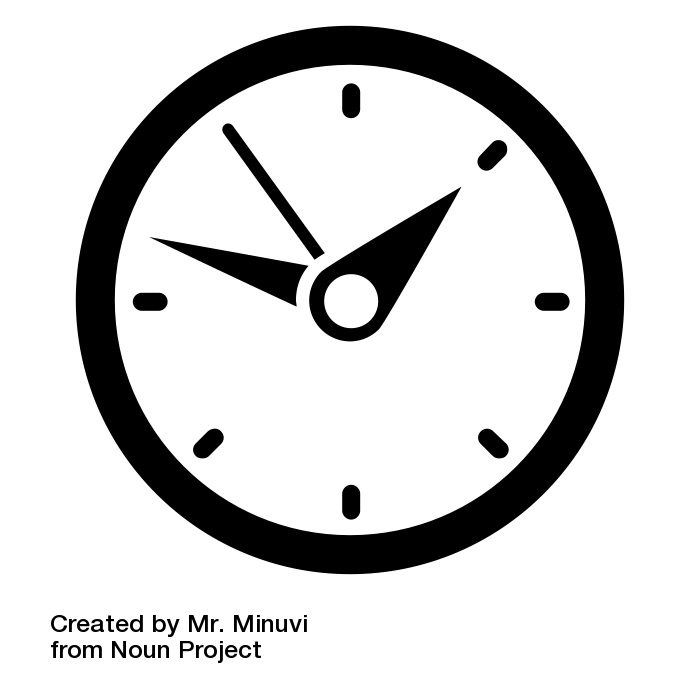
\includegraphics[width=0.9\textwidth]{symbols/symbol_tex_time}
				
				\begin{center}
					\textbf{135min} % Zeitangabe für Lernende // study time for students 
				\end{center}
			\end{tcolorbox}
		\end{minipage}

\vspace{0.3cm}
		% *********************************************
		% empfohlene Wiederholung // recommended review  
		% *********************************************
		\begin{tcolorbox}[enhanced,
			colback=white,
			colframe=orange!60!red,
			fonttitle=\sffamily\bfseries\large, 
			title=Wiederholung,  % search keyword::Wiederholung
			attach boxed title to top left={xshift=3.2mm,yshift=-0.50mm},
			boxed title style={skin=enhancedfirst jigsaw,size=small,arc=1mm,bottom=-1mm,colframe=orange!60!red,height=0.75cm},
			colbacktitle=orange!60!red,
			% sharp corners,
			drop lifted shadow]	
			\begin{wrapfigure}{L}{0.15\textwidth}  
				\centering
				\vspace{-14pt}  % to align image with first line of text
				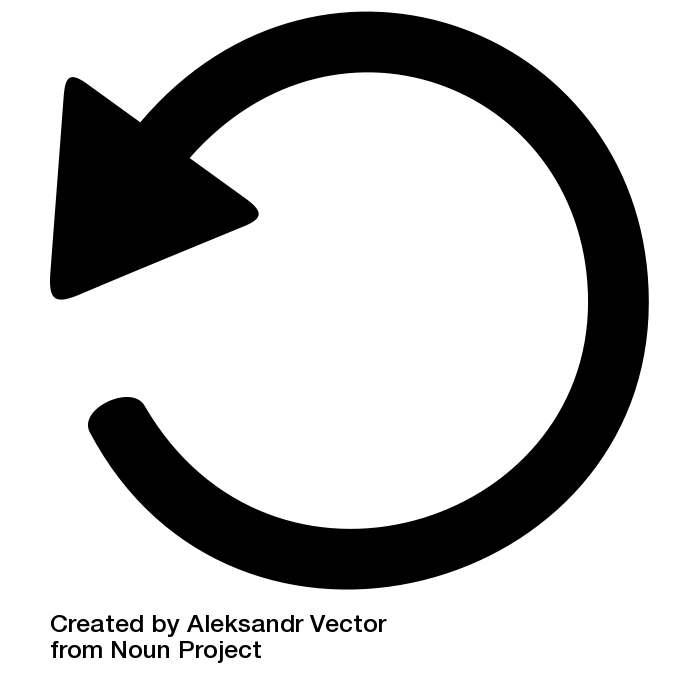
\includegraphics[width=0.9\textwidth]{symbols/symbol_tex_review}
			\end{wrapfigure}
			
			\textbf{Wiederholen Sie alle funktionellen Gruppen, die Sie bisher in der organischen Chemie im Unterricht kennengelernt haben. Erstellen Sie eine kleine Übersichtstabelle!}
			\vspace{1.3cm}
			
		\end{tcolorbox}
		% Layout: Linie zum Abgrenzen
		\begin{center}
			\noindent\rule{18cm}{0.1pt}
		\end{center}
	% *********************************************
	% Ende Kapitelübersicht // End Chapter Overview
	% *********************************************				
\newpage	
					
		\subsection{Maltose}
		
			\textbf{Auftrag: Informieren Sie sich über Maltose!}
			\begin{enumerate}
    			\item \textbf{Vervollständigen} Sie die gegebene Reaktionsgleichung (siehe unten) und \textbf{erläutern} Sie die Synthese und Struktur von Maltose aus den Monomerbausteinen!
			    \item \textbf{Nennen} Sie den Namen dieses speziellen Reaktionstypen.
% TODO: Dissacharide sollen angeblich keine Ether sein?! Nachprüfen!!!!
			    \item Disaccharide sind auf Grund ihrer Bidnung auch Ether. \textbf{Erklären} Sie warum.
			    \item \textbf{Nennen} Sie Vorkommen und Verwendung von Maltose!
			    \item Für die alkoholische Gärung benötigt man Glucose, keine Maltose. \textbf{Recherchieren} und \textbf{erläutern} Sie, wie aus der Maltose nun vergärbare Zucker hergestellt werden. 
			    \item In der Stärke unterscheiden sich Amylose und Amylopektin durch ihre glykosidischen Bindungen. \textbf{Recherchieren} und \textbf{erläutern} Sie den Unterschied.
			\end{enumerate}					

\vspace{0.3cm}
			\begin{tcolorbox}[enhanced,
				colback=white,
				colframe=darkgray,
				fonttitle=\sffamily\bfseries\large, 
				title=Maltose,  % search keyword::Informationstexte 
				attach boxed title to top left={xshift=3.2mm,yshift=-0.50mm},
				boxed title style={skin=enhancedfirst jigsaw,size=small,arc=1mm,bottom=-1mm,colframe=darkgray,height=0.75cm},
				colbacktitle=darkgray,
				drop lifted shadow]
				\begin{wrapfigure}{L}{0.15\textwidth}  
					\centering
					\vspace{-14pt}  % to align image with first line of text
					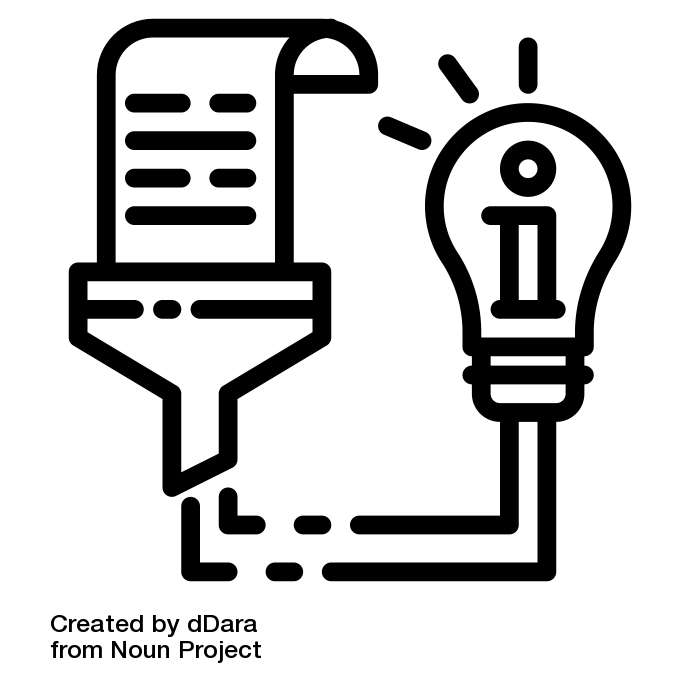
\includegraphics[width=0.9\textwidth]{symbols/symbol_tex_content}
				\end{wrapfigure}
				
				Maltose wird auch Malzzucker genannt und ist aus zwei α-D-Glucosebausteinen aufgebaut. Maltose kommt in Wurzeln und Knollen verschiedener Pflanzen vor und ist Bestandteil des Malzes, das man aus Gerstenkeimen erhält. Bei diesem Vorgang wird die in den Körnern enthaltene Stärke durch Enzyme gespalten. Die Maltose dient als Nahrung für die keimende Pflanze. Beim Bierbrauen ist dies ein wichtiger Arbeitsschritt. \newline
				Die beiden $\alpha$-D-Glucosemoleküle sind 1,4-glycosidisch1 verknüpft\footnote{Sie werden sich bei den Monosacchariden noch ausführlicher mit der glykosidischen Bindung beschäftigen.}, d.h. die Wasserabspaltung erfolgt zwischen der OH-Gruppe am C1-Atom des ersten Glucosemoleküls und der alkoholischen OH-Gruppe am C4-Atom des zweiten. Am C1-Atom des zweiten Glucosemoleküls verbleibt somit eine OH-Gruppe, die wiederum für den Aufbau längerer Zuckermoleküle (z.B. Oligosaccharide) genutzt werden kann.
				
			\end{tcolorbox}

\vspace{0.3cm}
			\noindent \textbf{Reaktionsgleichung zur Synthese von Maltose aus den Monomerbausteinen:} \newline

			\begin{minipage}{0.7\textwidth}
				\includegraphics{images/alpha_d_glucose}
			\end{minipage}
			\begin{minipage}{0.2\textwidth}
				\ch{->}
			\end{minipage}
			
		\subsection{Lactose und Saccharose}
		
			\textit{Neben der Maltose gibt es natürlich noch viele weitere Beispiele für Disaccharide. Die Bekanntesten sind die Saccharose und die Lactose.} \newline
			
			\noindent \textbf{Auftrag: Informieren Sie sich und Ihre MitschülerInnen über Lactose!}
			\begin{enumerate}
				    \item Erläutern Sie anhand einer Reaktionsgleichung die Synthese und die Struktur von Lactose aus den Monomerbausteinen!
				    \item  Nennen Sie Vorkommen und Verwendung von Lactose!
				    \item  Präsentieren Sie ihre Ergebnisse Ihren MitschülerInnen!
				    \item  Erstellen sie zusammen eine tabellarische Lernübersicht (Formel, Struktur, Bindungen, Verwendung) über alle drei Disaccharide. 
			\end{enumerate}

\vspace{0.3cm}
			\begin{tcolorbox}[enhanced,
				colback=white,
				colframe=darkgray,
				fonttitle=\sffamily\bfseries\large, 
				title=Lactose,  % search keyword::Informationstexte 
				attach boxed title to top left={xshift=3.2mm,yshift=-0.50mm},
				boxed title style={skin=enhancedfirst jigsaw,size=small,arc=1mm,bottom=-1mm,colframe=darkgray,height=0.75cm},
				colbacktitle=darkgray,
				drop lifted shadow]
				\begin{wrapfigure}{L}{0.15\textwidth}  
					\centering
					\vspace{-14pt}  % to align image with first line of text
					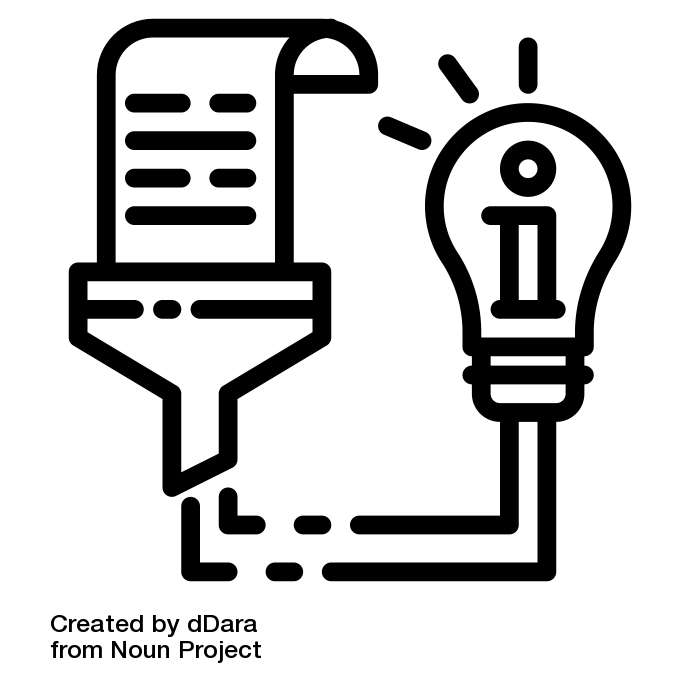
\includegraphics[width=0.9\textwidth]{symbols/symbol_tex_content}
				\end{wrapfigure}
				
				Lactose heißt auch Milchzucker und ist in der Muttermilch von Säugetieren, also auch vom Menschen, enthalten. Sie ist daher Bestandteil vieler Milchprodukte. Lactosemoleküle bestehen aus einem $\beta$-D-Galactosemolekül und einem D-Glucosemolekül. Die Bausteine sind β-1,4-glycosidisch verknüpft, d.h. die Wasserabspaltung erfolgt zwischen der halbacetalischen OH-Gruppe am C1-Atom des Galactosemoleküls und der alkoholischen OH-Gruppe am C4-Atom des Glucosemoleküls. Am C1-Atom des Glucosemoleküls verbleibt somit eine halbacetalische OH-Gruppe. 
				Zur Verwertung der Lactose im Organismus muss sie durch das Verdauungsenzym Lactase in die beiden Monosaccharide gespalten werden. Kann Lactose aufgrund eines Mangels an Lactase (im Dünndarm) nicht verdaut werden und gelangt ungespalten in den Dickdarm, so wird sie von Darmbakterien vergoren, was u.a. zu Blähungen und Durchfall führt (Lactoseintoleranz). Inzwischen werden zahlreiche lactosefreie Milchprodukte angeboten.
				
			\end{tcolorbox}		
			
\vspace{0.3cm}
			\noindent \textbf{Auftrag: Informieren Sie sich und Ihre MitschülerInnen über Saccharose!}
			\begin{enumerate}
			     \item Erläutern Sie anhand einer Reaktionsgleichung die Synthese und die Struktur von Saccharose aus den Monomerbausteinen!
			     \item Nennen Sie Vorkommen und Verwendung von Saccharose!
			     \item Besprechen Sie die Darstellung der Saccharose mit der Lehrerkraft!
			     \item Präsentieren Sie ihre Ergebnisse Ihren MitschülerInnen!
			     \item Erstellen sie zusammen eine tabellarische Lernübersicht (Formel, Struktur, Bindungen, Verwendung) über alle drei Disaccharide.
			\end{enumerate}

\vspace{0.3cm}
			\begin{tcolorbox}[enhanced,
				colback=white,
				colframe=darkgray,
				fonttitle=\sffamily\bfseries\large, 
				title=Saccharose,  % search keyword::Informationstexte 
				attach boxed title to top left={xshift=3.2mm,yshift=-0.50mm},
				boxed title style={skin=enhancedfirst jigsaw,size=small,arc=1mm,bottom=-1mm,colframe=darkgray,height=0.75cm},
				colbacktitle=darkgray,
				drop lifted shadow]
				\begin{wrapfigure}{L}{0.15\textwidth}  
					\centering
					\vspace{-14pt}  % to align image with first line of text
					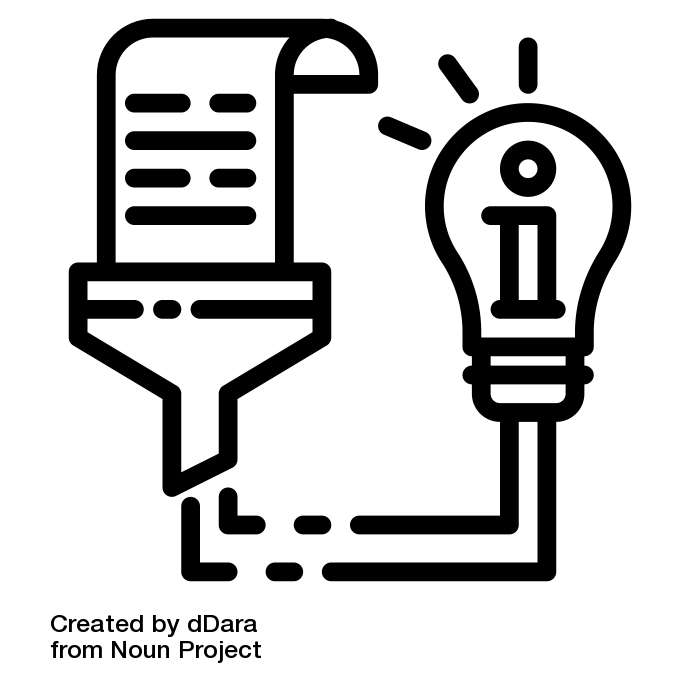
\includegraphics[width=0.9\textwidth]{symbols/symbol_tex_content}
				\end{wrapfigure}
				
				Saccharose, der „normale“ Haushaltszucker, ist das wichtigste und am häufigsten vorkommende Disaccharid. Es findet sich in fast allen Früchten und in vielen Pflanzensäften, vor allem im Zuckerrohr (14-16\%) und in Zuckerrüben (16-20\%). Aus diesen Pflanzen wird Saccharose in großen Mengen gewonnen und gelangt als Rohr- oder Rübenzucker in den Handel. Bei der Hydrolyse von Saccharose erhält man Glucose und Fructose. Durch Röntgenstrukturanalyse kann gezeigt werden, dass im Saccharosemolekül der Glucoserest als 6-Ring ($\alpha$-Pyranose) und der Fructoserest ungewöhnlicherweise als 5-Ring ($\beta$-Furanose), vorliegt. Diese sind über die OH-Gruppen der anomeren C-Atome (C1-Atom Glucose und C2-Atom Fructose) miteinander verbunden. In einer Kondensationsreaktion entsteht also eine 1,2-glycosidische Bindung. 
				Um die Bildung der glycosidischen Bindung besser zu verstehen, schreibt man sich die Glucose und Fructose in der Haworth-Projektion meistens nebeneinander. Bei der Glucose ist die OH-Gruppe des anomeren C-Atom in der $\alpha$-Stellung , bei der Fructose in der $\beta$-Stellung. Zur Ausbildung der Bindung muss das Fructosemolekül um 180° gedreht werden, welche durch das O-Atom und die Mitte der Bindung zwischen den C-Atomen 3 und 4 geht.
				
			\end{tcolorbox}				

\newpage

				
				% ***** start copy here *********************************************************
				% *******************************************************************************
				%            __ _           _   _                        _                _   
				%  _ __ ___ / _| | ___  ___| |_(_) ___  _ __         ___| |__   __ _ _ __| |_ 
				% | '__/ _ \ |_| |/ _ \/ __| __| |/ _ \| '_ \ _____ / __| '_ \ / _` | '__| __|
				% | | |  __/  _| |  __/ (__| |_| | (_) | | | |_____| (__| | | | (_| | |  | |_ 
				% |_|  \___|_| |_|\___|\___|\__|_|\___/|_| |_|      \___|_| |_|\__,_|_|   \__|
				%                                                                            
				%
				
				\vspace{0.3cm}
				\begin{center}
					\begin{tcolorbox}[enhanced,
						width=0.75\textwidth,
						colback=white,
						colframe=darkgray,
						fonttitle=\sffamily\bfseries\large, 
						title=Kurzreflexion,  % search keyword::Informationstexte 
						attach boxed title to top left={xshift=3.2mm,yshift=-0.50mm},
						boxed title style={skin=enhancedfirst jigsaw,size=small,arc=1mm,bottom=-1mm,colframe=darkgray,height=0.75cm},
						colbacktitle=darkgray,
						drop lifted shadow]
						
						% \begin{figure}[htbp]  % not good in ecolorbox
						\textbf{Auftrag: Bewerten Sie Ihre Arbeit in der letzten Einheit selbst.} \newline
						\begin{center}
							\begin{tikzpicture}[scale=1]
								\path (0:0cm) coordinate (O); % define coordinate for origin
								
								% draw the spiderweb
								\foreach \X in {1,...,\D}{
									\draw (\X*\A:0) -- (\X*\A:\R);
								}
								
								\foreach \Y in {0,...,\U}{
									\foreach \X in {1,...,\D}{
								\path (\X*\A:\Y*\R/\U) coordinate (D\X-\Y);
								\fill (D\X-\Y) circle (1pt);
									}
									\draw [opacity=0.3] (0:\Y*\R/\U) \foreach \X in {1,...,\D}{
										-- (\X*\A:\Y*\R/\U)
									} -- cycle;
								}
								
								% define labels for each dimension axis (names config option)
								\path (1*\A:\L) node (L1) {\tiny Verständnis};
								\path (2*\A:\L) node (L2) {\tiny alle Aufgaben gelöst};
								\path (3*\A:\L) node (L3) {\tiny Zeit effektiv genutz};
								\path (4*\A:\L) node (L4) {\tiny Einzelarbeit};
								\path (5*\A:\L) node (L5) {\tiny Gruppenarbeit};
							
							\end{tikzpicture}
							% \caption{Diagramm Slebstreflexion}
							% \caption{Spiderweb Diagram (\D~Dimensions, \U-Notch Scale, 3 Samples)}
							% \label{fig:spiderweb}
							% \end{figure} 
						\end{center}
						\textbf{{\Large Was können Sie in der nächsten Stunde verbessern?}}
						\begin{center}
							%\vspace{1.1cm}
							\noindent\rule{12cm}{0.2pt}
							\vspace{1.1cm}
							\noindent\rule{12cm}{0.1pt}
							\vspace{1.1cm}
							\noindent\rule{12cm}{0.1pt}
							\vspace{1.1cm}
							\noindent\rule{12cm}{0.1pt}
							\vspace{1.1cm}
							\noindent\rule{12cm}{0.1pt}
							\vspace{1.1cm}
							\noindent\rule{12cm}{0.1pt}
							\vspace{1.1cm}
							\noindent\rule{12cm}{0.1pt}
							\vspace{1.1cm}
							\noindent\rule{12cm}{0.1pt}
						\end{center}
					\end{tcolorbox}
				\end{center}
								
				% *******************************************************************************
				% ***** end copy here ***********************************************************

\newpage	
	\part{Die Monomerbausteine der Polysaccharide (Zucker)}
	
		\textit{Bei der Recherche zu den Dissachariden sind ihnen vielleicht viele Begriffe zu den Strukturen begegnet, die nicht gleich erklärt wurden. Dies soll nun hier geschehen. Für das Brauen ist am Ende die Glucose das wichtigste Molekül, da es für die Gärung entscheidend ist. An diesem Molekül sollen Sie also die Darstellungen, Bindungen und Eigenschaften erarbeiten.} \newline

	\section{Die FISCHER-Projektion}

		\textit{Aus der Strukturanalyse der Glucose ergibt sich, dass das Molekül eine Aldehydgruppe und sechs Hydroxylgruppen enthält. Um Moleküle dieser Art darzustellen, benötigt man eine einfache und übersichtliche Darstellung. Diese wurde von Hermann Emil Fischer vorgeschlagen. } \newline
	
		\begin{minipage}{0.7\textwidth}
			% *******************************
			% Übersicht Lernziele // Overview  
			% *******************************
			\noindent \textbf{Am Ende dieses Kapitels sollen Sie ... :}
			\begin{enumerate}
				\item ... die Regeln zum Aufstellen der Fischer-Projektion erklären können.
				\item ... ein Glucose-Molekül mit Hilfe dieser Projektion darstellen können.
				\item ... die Unterscheidung von Enantiomeren erläutern können.
			\end{enumerate}
			% *************************************************
			% empfohlene Vorgehensweise // recommended approach  
			% *************************************************
			% Lernende können selbst entscheiden, wie sie sich durch das Kapitel arbeiten
			% Lehrpersonen/Lernende können folgende Empfehlung aber nutzen
			\textbf{Vorgehensweise:}
			\begin{enumerate}
				\item Arbeiten Sie erst einmal allein.
				\item Lesen Sie den Text und bearbeiten Sie den Arbeitsaufträge.
				\item Vergleichen Sie mit Ihren Mitschülern.
				\item Erweitern Sie die Mind-Maps aus den ersten Kapiteln. 
			\end{enumerate}
			
		\end{minipage}
		\hspace{0.1\textwidth}
		% ***********************************
		% empfohlene Zeit // recommended time  
		% ***********************************
		% zeitliche Orientierung für Lernende und Lehrpersonen
		% Zeit sollte aber ungefährt eingehalten werden, damit Reihenplanung funktioniert
		\begin{minipage}{0.2\textwidth}
			\begin{tcolorbox}
				[enhanced,
				width=0.9\textwidth,
				colback=white,
				colframe=black,
				fonttitle=\sffamily\bfseries\large, 
				title=Zeit,  % search keyword::Zeit
				attach boxed title to top center={xshift=-0.0mm,yshift=-0.50mm},
				boxed title style={skin=enhancedfirst jigsaw,size=small,arc=1mm,bottom=-1mm,colframe=black,height=0.75cm},
				colbacktitle=black,
				drop lifted shadow]
				\centering
				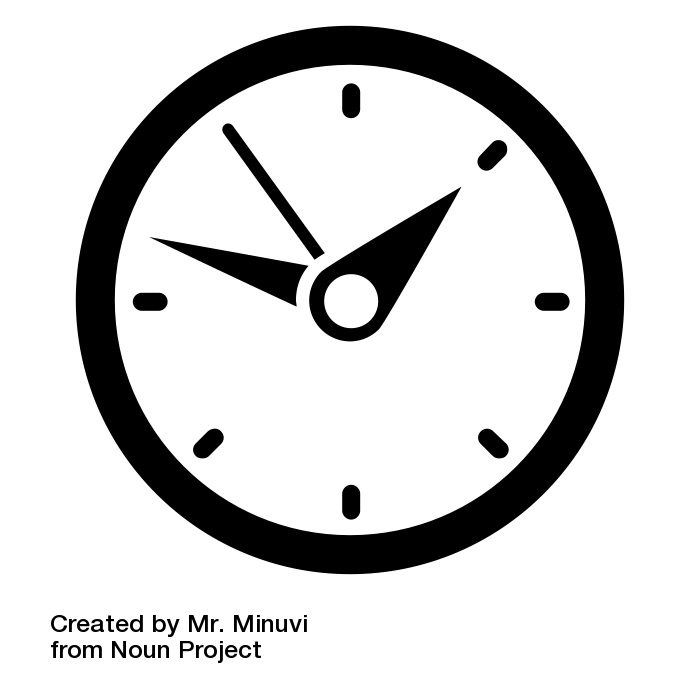
\includegraphics[width=0.9\textwidth]{symbols/symbol_tex_time}
				
				\begin{center}
					\textbf{90min} % Zeitangabe für Lernende // study time for students 
				\end{center}
			\end{tcolorbox}
		\end{minipage}

\vspace{0.3cm}
		% *********************************************
		% empfohlene Wiederholung // recommended review  
		% *********************************************
		\begin{tcolorbox}[enhanced,
			colback=white,
			colframe=orange!60!red,
			fonttitle=\sffamily\bfseries\large, 
			title=Wiederholung,  % search keyword::Wiederholung
			attach boxed title to top left={xshift=3.2mm,yshift=-0.50mm},
			boxed title style={skin=enhancedfirst jigsaw,size=small,arc=1mm,bottom=-1mm,colframe=orange!60!red,height=0.75cm},
			colbacktitle=orange!60!red,
			% sharp corners,
			drop lifted shadow]	
			\begin{wrapfigure}{L}{0.15\textwidth}  
				\centering
				\vspace{-14pt}  % to align image with first line of text
				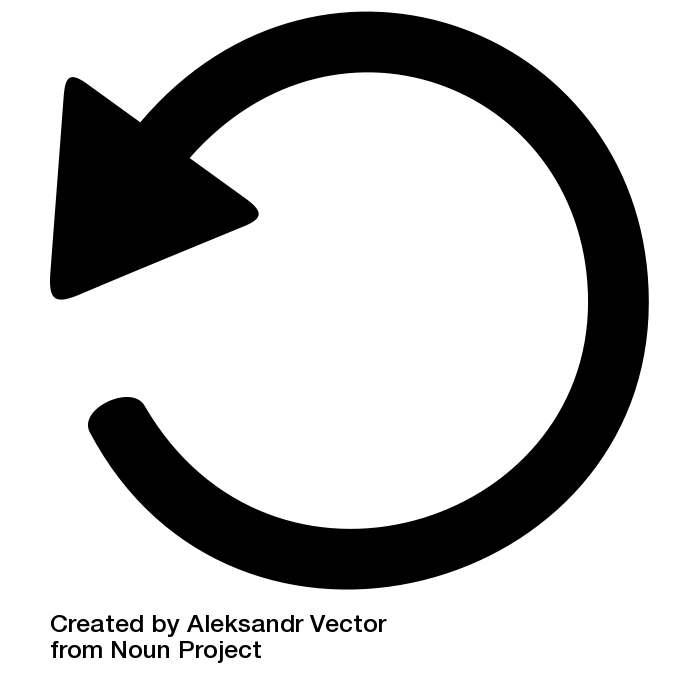
\includegraphics[width=0.9\textwidth]{symbols/symbol_tex_review}
			\end{wrapfigure}
			
			\textbf{Erklären Sie den Begriff \textit{Oxidationszahlen}. Nennen Sie die Regeln, die man beim Aufstellen der Oxidationszahlen beachten muss.}
			\vspace{1.3cm}
			
		\end{tcolorbox}
		% Layout: Linie zum Abgrenzen
		\begin{center}
			\noindent\rule{18cm}{0.1pt}
		\end{center}
	% *********************************************
	% Ende Kapitelübersicht // End Chapter Overview
	% *********************************************				
\newpage	
		\subsection{Die Regeln für die FISCHER-Projektion}
		
			\textbf{Auftrag: Recherchieren Sie die Regeln zum Zeichnen der FISCHER-Projetion.}
		
		\subsection{Die Strukturformel der D-Glucose}
			
			\textbf{Auftrag: Lösen Sie mit Hilfe der Fischer-Projektion die folgenden Aufgaben!}
			
			\begin{enumerate}
				\item \textbf{Erläutern} Sie den Begriff \textit{asymmetrisches C-Atom} und \textit{Chiralitätszentrum}! Wie werden diese Atome in der Fischer-Projektion gekennzeichnet?
				\item Im D-Glucose-Molekül sind die vier Hydroxylgruppen an den asymmetrischen C-Atomen nicht alle auf einer Seite angeordnet. Man kann sich die Anordnung mit der Eselsbrücke „Ta(Rechts)-Tü(Links)-Ta-Ta“ merken. Zeichnen Sie das Molekül der D-Glucose.
			\end{enumerate}
			
		\subsection{Enantiomere}
			
			\textit{Bisher haben Sie sich mit der D-Glucose beschäftigt. Aber was bedeutet das D eigentlich? Und gibt es auch noch andere Arten von Glucose?} \newline
			
			\noindent \textbf{Auftrag: Erläutern Sie, warum es sich bei Glucose um ein Enantiomer handelt.}
			\begin{enumerate}
				\item \textbf{Lesen} Sie den Text.
				\item \textbf{Zeichnen} Sie die Enantiomere des Glycerinaldehyds (C-Atome vertikal)
					\begin{itemize}
						\item Erstellen Sie eine zweispaltige Tabelle (s.u.). Zeichnen Sie jeweils ein Enantiomer in die Spalten.
						\item \textbf{Kennzeichnen} Sie das asymmetrische Kohlenstoffatom!
						\item \textbf{Kennzeichnen} Sie die Moleküle mit D bzw. L!
					\end{itemize}
				\item \textbf{Entwickeln} Sie aus der jeweiligen Glycerinaldehydform schrittweise die D- bzw. L- Glucose. Fügen Sie dazu immer eine H-C-OH Gruppe ein.
					\begin{itemize}
						\item Ergänzen Sie dafür die Tabelle Zeile um Zeile.
						\item \textbf{Kennzeichnen} Sie die neue Gruppe, indem Sie sie farbig von dem Rest des Moleküls unterscheiden. Denken Sie an Ta-Tü-Ta-Ta!
					\end{itemize} 
			\end{enumerate}
			
			\begin{center}
				\begin{tabular}{|c|c|}
					\hline
					... -Glycerinaldehyd & ... -Glycerinaldehyd \\
					\hline
					... & ... \\
					\hline
				\end{tabular}
			\end{center}

\vspace{0.3cm}
			\begin{tcolorbox}[enhanced,
				colback=white,
				colframe=darkgray,
				fonttitle=\sffamily\bfseries\large, 
				title=Enantiomere,  % search keyword::Informationstexte 
				attach boxed title to top left={xshift=3.2mm,yshift=-0.50mm},
				boxed title style={skin=enhancedfirst jigsaw,size=small,arc=1mm,bottom=-1mm,colframe=darkgray,height=0.75cm},
				colbacktitle=darkgray,
				drop lifted shadow]
				\begin{wrapfigure}{L}{0.15\textwidth}  
					\centering
					\vspace{-14pt}  % to align image with first line of text
					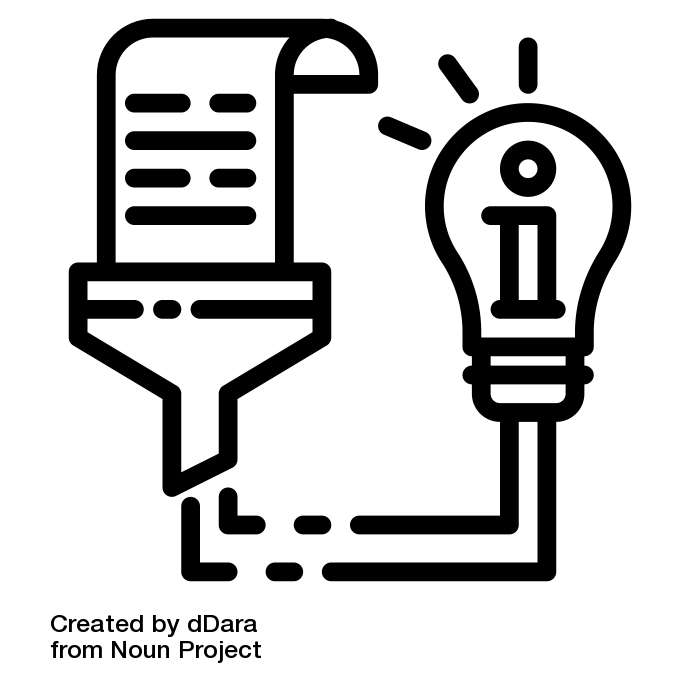
\includegraphics[width=0.9\textwidth]{symbols/symbol_tex_content}
				\end{wrapfigure}
				
				Die beiden Formen eines Moleküls, die sich wie Bild und Spiegelbild zueinander verhalten, bezeichnet man als enantiomer zueinander, sie bilden zusammen ein Enantiomerenpaar. Prof. Emil Fischer, der bahnbrechende Forschungen zur Strukturaufklärung bei Kohlenhydraten durchgeführt hat, machte auch einen Vorschlag, wie man Enantiomere eindeutig bezeichnen kann. \newline
				Als Bezugssystem verwendete er das einfachste Kohlenhydrat: Glycerinaldehyd (2,3-Dihydroxypropanal). Befindet sich die Hydroxylgruppe am asymmetrischen Kohlenstoffatom bei der Projektion des Moleküls in die Ebene auf der rechten Seite, handelt es sich um eine D-Form (lateinisch: dexter – rechts), befindet sie sich auf der linken Seite, liegt eine L-Form vor (lateinisch: laevus – links). Die Angabe der Konfiguration (D bzw. L) wird der Verbindungsbezeichnung vorangestellt. \newline
				Aufbauend auf diesem Molekül kann man nun zwischen die Aldehydgruppe und das asymmetrische Kohlenstoffatom weiter H-C-OH Gruppen einfügen. Somit erhält man dann jeweils die D- oder L-Form des entstehenden Moleküls.
				
			\end{tcolorbox}				

			\noindent \textbf{Auftrag: Vervollständigen Sie den Lernsatz.}
			
\vspace{0.3cm}
			{\fontfamily{qag}\selectfont  % set different font for chat-entry
			\begin{tcolorbox}[enhanced,
				colback=white,
				colframe=teal,
				fonttitle=\sffamily\bfseries\large, 
				title=Merksatz zu Enantiomeren, 
				attach boxed title to top left={xshift=3.2mm,yshift=-0.50mm},
				boxed title style={skin=enhancedfirst jigsaw,size=small,arc=1mm,bottom=-1mm,colframe=teal,height=0.6cm},
				colbacktitle=teal,
				drop lifted shadow]
				
				Für Moleküle mit mehreren Chiralitätszentren gilt folgende Regel: Die D/L-Schreibweise bezieht sich auf das asymmetrische C-Atom, das ........ vom höchst oxidierten Kohelnstoffatom (höchste Oxidationszahl) entfernt ist!
				% \vspace{1.3cm}  % to fill empty space in tcolorbox
			\end{tcolorbox}
			}  % end different font for chat entry
			
\vspace{0.3cm}
			\noindent \textbf{Auftrag: Recherchieren Sie die Fischer-Projektion der Fructose! Zeichnen Sie das Molekül}

\newpage
	\section{Chiralität - Bild und Spiegelbild}
	
		\textit{Im letzten Kapitel haben Sie sich bereits mit Bildern und Spiegelbildern auseinandergesetzt. Doch es gibt eine weitere Besonderheit in diesem Zusammenhang. Viele Moleküle, die als Bild und Spiegelbild vorliegen, kann man durch Drehungen in Deckung bringen. D.h., es handelt sich um das gleiche Molekül. Es gibt Moleküle, die sich nicht nicht in Deckung bringen lassen. Dies hat Auswirkungen auf die Chemie der Stoffe. Doch wie erkennt man solche Moleküle? Und gehören D- und L-Glucose auch dazu?} \newline

		\begin{minipage}{0.7\textwidth}
			% *******************************
			% Übersicht Lernziele // Overview  
			% *******************************
			\noindent \textbf{Am Ende dieses Kapitels sollen Sie ... :}
			\begin{enumerate}
				\item ... die Begriffe Chiralität, Spiegelbildisomere und Enantiomere erklären können.
				\item ... die Bedingungen für Chiralität erläutern können.
			\end{enumerate}
			% *************************************************
			% empfohlene Vorgehensweise // recommended approach  
			% *************************************************
			% Lernende können selbst entscheiden, wie sie sich durch das Kapitel arbeiten
			% Lehrpersonen/Lernende können folgende Empfehlung aber nutzen
			\textbf{Vorgehensweise:}
			\begin{enumerate}
				\item Arbeiten Sie in Gruppen.
				\item Nutzen Sie Molekülbaukästen um die Aufträge zu bearbeiten.
				\item Erweitern Sie die Mind-Maps aus den ersten Kapiteln. 
			\end{enumerate}
			
		\end{minipage}
		\hspace{0.1\textwidth}
		% ***********************************
		% empfohlene Zeit // recommended time  
		% ***********************************
		% zeitliche Orientierung für Lernende und Lehrpersonen
		% Zeit sollte aber ungefährt eingehalten werden, damit Reihenplanung funktioniert
		\begin{minipage}{0.2\textwidth}
			\begin{tcolorbox}
				[enhanced,
				width=0.9\textwidth,
				colback=white,
				colframe=black,
				fonttitle=\sffamily\bfseries\large, 
				title=Zeit,  % search keyword::Zeit
				attach boxed title to top center={xshift=-0.0mm,yshift=-0.50mm},
				boxed title style={skin=enhancedfirst jigsaw,size=small,arc=1mm,bottom=-1mm,colframe=black,height=0.75cm},
				colbacktitle=black,
				drop lifted shadow]
				\centering
				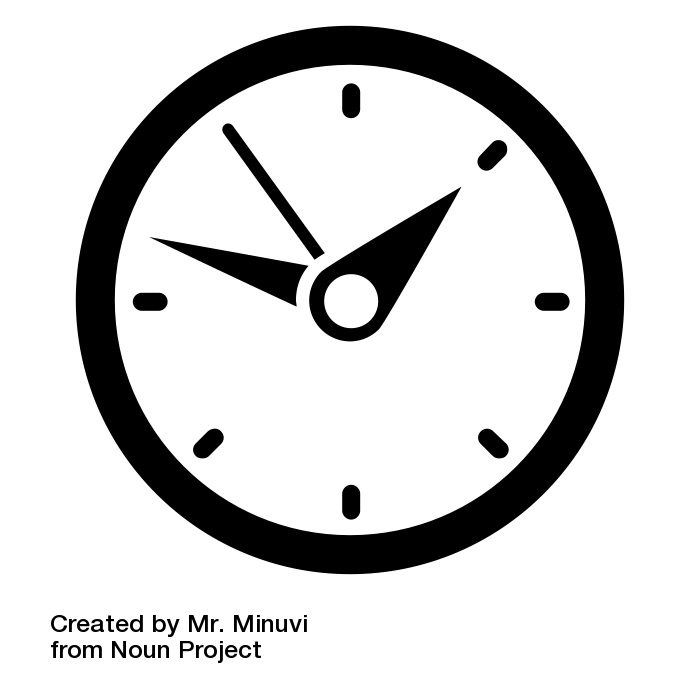
\includegraphics[width=0.9\textwidth]{symbols/symbol_tex_time}
				
				\begin{center}
					\textbf{90min} % Zeitangabe für Lernende // study time for students 
				\end{center}
			\end{tcolorbox}
		\end{minipage}

\vspace{0.3cm}
		% *********************************************
		% empfohlene Wiederholung // recommended review  
		% *********************************************
		\begin{tcolorbox}[enhanced,
			colback=white,
			colframe=orange!60!red,
			fonttitle=\sffamily\bfseries\large, 
			title=Vorüberlegung,  % search keyword::Wiederholung
			attach boxed title to top left={xshift=3.2mm,yshift=-0.50mm},
			boxed title style={skin=enhancedfirst jigsaw,size=small,arc=1mm,bottom=-1mm,colframe=orange!60!red,height=0.75cm},
			colbacktitle=orange!60!red,
			% sharp corners,
			drop lifted shadow]	
			\begin{wrapfigure}{L}{0.15\textwidth}  
				\centering
				\vspace{-14pt}  % to align image with first line of text
				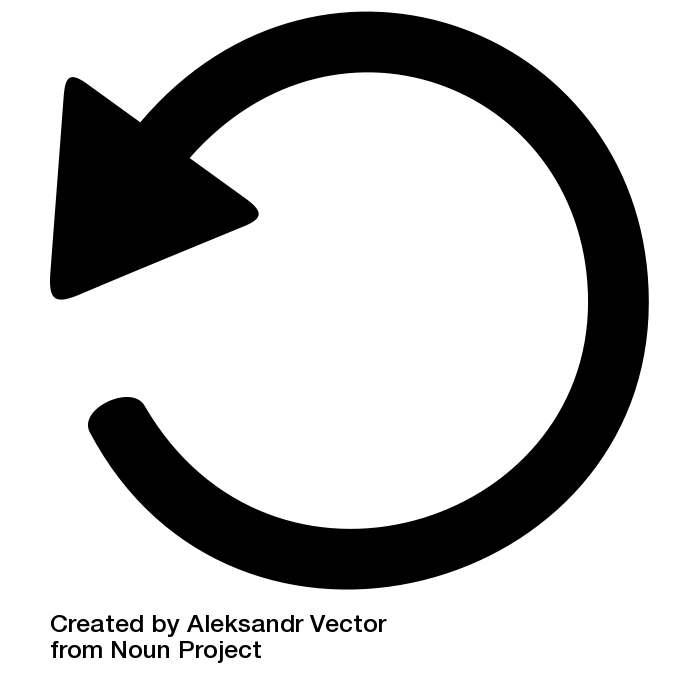
\includegraphics[width=0.9\textwidth]{symbols/symbol_tex_review}
			\end{wrapfigure}
			
			\textbf{Versuchen Sie Ihre Hände in Deckung zu bringen.}
			\vspace{1.7cm}
			
		\end{tcolorbox}
		% Layout: Linie zum Abgrenzen
		\begin{center}
			\noindent\rule{18cm}{0.1pt}
		\end{center}
	% *********************************************
	% Ende Kapitelübersicht // End Chapter Overview
	% *********************************************				
\newpage
		\subsection{Herleitung der Chiralität}	
			\begin{tcolorbox}[enhanced,
				colback=white,
				colframe=darkgray,
				fonttitle=\sffamily\bfseries\large, 
				title=Enantiomere,  % search keyword::Informationstexte 
				attach boxed title to top left={xshift=3.2mm,yshift=-0.50mm},
				boxed title style={skin=enhancedfirst jigsaw,size=small,arc=1mm,bottom=-1mm,colframe=darkgray,height=0.75cm},
				colbacktitle=darkgray,
				drop lifted shadow]
				\begin{wrapfigure}{L}{0.15\textwidth}  
					\centering
					\vspace{-14pt}  % to align image with first line of text
					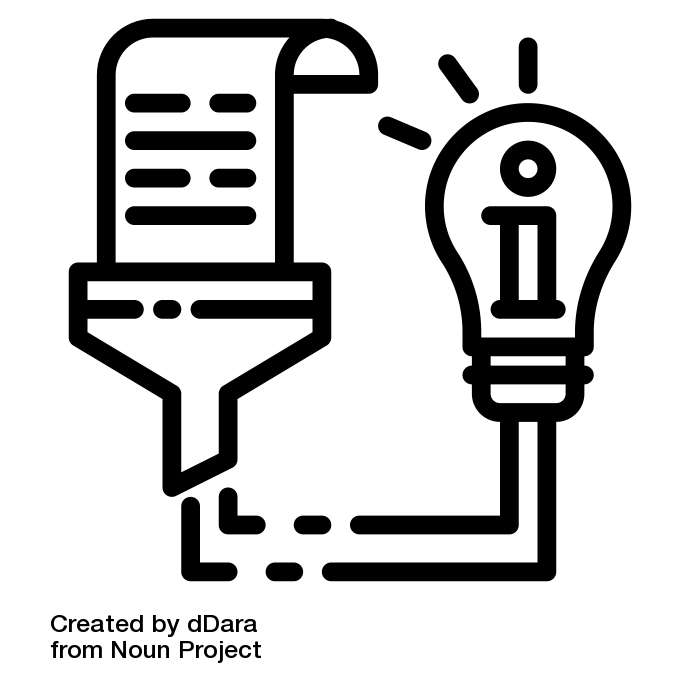
\includegraphics[width=0.9\textwidth]{symbols/symbol_tex_content}
				\end{wrapfigure}
				
				Chiralität (abgeleitet vom griechischen Wortstamm ch[e]ir~ – hand~) steht für die Eigenschaft, dass Bild und Spiegelbild eines Gegenstandes nicht zur Deckung gebracht werden können (wie Ihre beiden Hände!). Gegenstände, die diese Eigenschaft besitzen, bezeichnet man als chiral. \newline
				Moleküle, die sich so verhalten, nennt man Spiegelbildisomere oder Enantiomere. 
				
			\end{tcolorbox}				
			
\vspace{0.3cm}
			\noindent \textbf{Auftrag: Erabeiten Sie sich mit Hilfe des Molekülbaukastens und des Arbeitsblattes die Bedingung für die Chiralität!}
			\begin{enumerate}
    			\item Bauen Sie zwei Methanmoleküle (C-Atom: schwarz, H-Atom: weiß)!
    			\item Übernehmen Sie die Strukturen (möglichst) dreidimensional in Ihre Notizen (z.B. Tabelle).
    			\item Ersetzen Sie dann jeweils ein Wasserstoffatom durch eine andere Atomsorte. Prüfen Sie, ob sich die beiden Moleküle in Deckung bringen lassen!
    			\item Ersetzen Sie jetzt ein weiteres Wasserstoffatom durch eine andere Atomsorte (noch anders als in Schritt 2). Prüfen Sie wieder auf Chiralität!
    			\item Ersetzen Sie ein weiteres Wasserstoffatom. Prüfen Sie erneut auf Chiralität.
    			\item Formulieren eine Regel mit deren Hilfe man Enantiomere erkennt!
			\end{enumerate}

			\begin{tabular}{|c|c|c|}
				\hline
				Modell 1 & Modell 2 & Chiralität (j\/n) \\
				\hline
				\includegraphics[width=0.2\textwidth]{images/methan1} &
				\includegraphics[width=0.2\textwidth]{images/methan2} &
				... \\
				\hline
			\end{tabular}

\newpage
	\section{Optische Aktivität}
	
		\textit{Das Phänomen der Optischen Aktivität kennen wahrscheinlich viele Menschen durch die Werbung oder wenn sie die Lebensmittelverpackungen lesen. Links oder Rechtsdrehende Joghurtkulturen sollen gut für die Gesundheit sein. Aber was bedeutet das? Das Phänomen lässt sich aber auch für die Analyse von chemischen Substanzen nutzen. Dabei haben die chiralen Zentren eine besondere Aufgabe.} \newline

		\begin{minipage}{0.7\textwidth}
			% *******************************
			% Übersicht Lernziele // Overview  
			% *******************************
			\noindent \textbf{Am Ende dieses Kapitels sollen Sie ... :}
			\begin{enumerate}
				\item ... den Begriff Optische Aktivität erklären können.
				\item ... Berechnungen mit Hilfe der optischen Aktivität durchführen können.
			\end{enumerate}
			% *************************************************
			% empfohlene Vorgehensweise // recommended approach  
			% *************************************************
			% Lernende können selbst entscheiden, wie sie sich durch das Kapitel arbeiten
			% Lehrpersonen/Lernende können folgende Empfehlung aber nutzen
			\textbf{Vorgehensweise:}
			\begin{enumerate}
				\item Arbeiten Sie erst einmal allein.
				\item Bearbeiten Sie die Aufgaben in den Vorüberlegungen!
				\item Bearbeiten Sie alle Arbeitsaufträge.
				\item Vergleichen Sie Ihre Resultate mit ihren MitschülerInnen und den Lösungen!
				\item Erweitern Sie die Mind-Maps aus den ersten Kapiteln. 
			\end{enumerate}
			
		\end{minipage}
		\hspace{0.1\textwidth}
		% ***********************************
		% empfohlene Zeit // recommended time  
		% ***********************************
		% zeitliche Orientierung für Lernende und Lehrpersonen
		% Zeit sollte aber ungefährt eingehalten werden, damit Reihenplanung funktioniert
		\begin{minipage}{0.2\textwidth}
			\begin{tcolorbox}
				[enhanced,
				width=0.9\textwidth,
				colback=white,
				colframe=black,
				fonttitle=\sffamily\bfseries\large, 
				title=Zeit,  % search keyword::Zeit
				attach boxed title to top center={xshift=-0.0mm,yshift=-0.50mm},
				boxed title style={skin=enhancedfirst jigsaw,size=small,arc=1mm,bottom=-1mm,colframe=black,height=0.75cm},
				colbacktitle=black,
				drop lifted shadow]
				\centering
				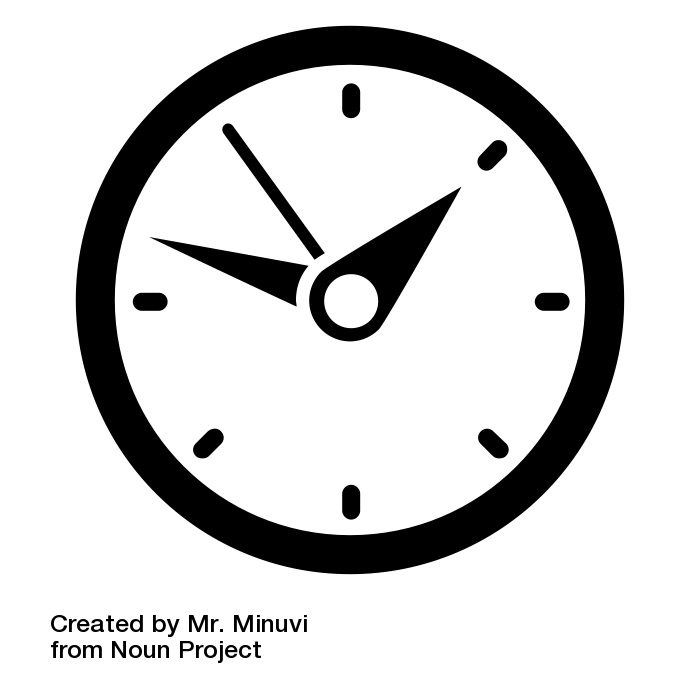
\includegraphics[width=0.9\textwidth]{symbols/symbol_tex_time}
				
				\begin{center}
					\textbf{90min} % Zeitangabe für Lernende // study time for students 
				\end{center}
			\end{tcolorbox}
		\end{minipage}

\vspace{0.3cm}
		% *********************************************
		% empfohlene Wiederholung // recommended review  
		% *********************************************
		\begin{tcolorbox}[enhanced,
			colback=white,
			colframe=orange!60!red,
			fonttitle=\sffamily\bfseries\large, 
			title=Vorüberlegung,  % search keyword::Wiederholung
			attach boxed title to top left={xshift=3.2mm,yshift=-0.50mm},
			boxed title style={skin=enhancedfirst jigsaw,size=small,arc=1mm,bottom=-1mm,colframe=orange!60!red,height=0.75cm},
			colbacktitle=orange!60!red,
			% sharp corners,
			drop lifted shadow]	
			\begin{wrapfigure}{L}{0.15\textwidth}  
				\centering
				\vspace{-14pt}  % to align image with first line of text
				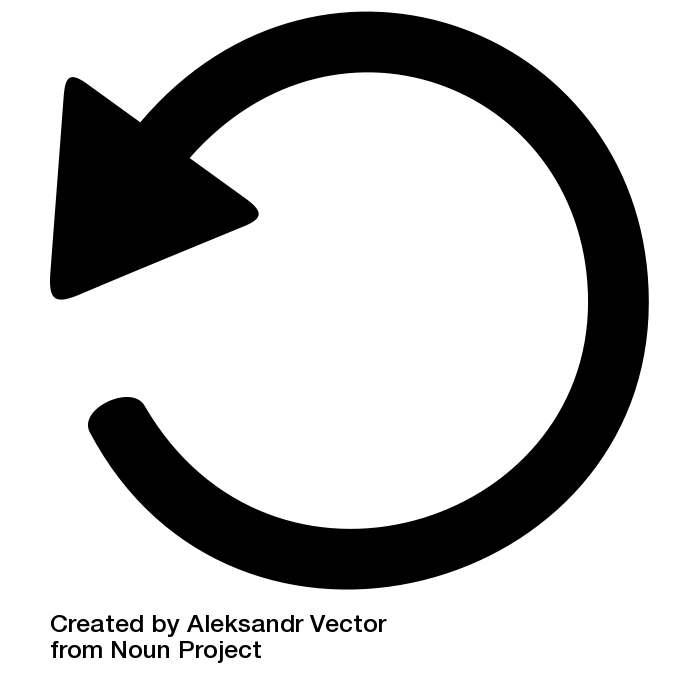
\includegraphics[width=0.9\textwidth]{symbols/symbol_tex_review}
			\end{wrapfigure}
			
			\textbf{Erklären} Sie was der Welle-Teilchen-Dualismus des Lichtes ist. \textbf{Erklären} Sie, wie eine 3D-Brille im Kino funktioniert.
			\vspace{1.3cm}
			
		\end{tcolorbox}
		% Layout: Linie zum Abgrenzen
		\begin{center}
			\noindent\rule{18cm}{0.1pt}
		\end{center}
	% *********************************************
	% Ende Kapitelübersicht // End Chapter Overview
	% *********************************************				
\newpage
		\subsection{Milchsäure}

			Sie sind gerade im Supermarkt und wollen sich eigentlich nur eine Milch kaufen. Plötzlich sehen Sie einen Joghurtbecher auf dem steht: Joghurt mit rechtsdrehender Milchsäure (L+). Irgendwie kommt Ihnen das bekannt vor. Hatten wir nicht im Chemieunterricht gelernt, dass es L-und D-Glucose gibt? Gibt es auch L- und D-Milchsäure? Und was bedeutet denn nun schon wieder rechtsdrehende Milchsäure? Gibt es auch eine linksdrehende Milchsäure? Sie fahren schnell nach Hause und finden folgendes bei der Recherche im Internet:

\vspace{0.3cm}
			\begin{tcolorbox}[enhanced,
				colback=white,
				colframe=darkgray,
				fonttitle=\sffamily\bfseries\large, 
				title=Recherche,  % search keyword::Informationstexte 
				attach boxed title to top left={xshift=3.2mm,yshift=-0.50mm},
				boxed title style={skin=enhancedfirst jigsaw,size=small,arc=1mm,bottom=-1mm,colframe=darkgray,height=0.75cm},
				colbacktitle=darkgray,
				drop lifted shadow]
				\begin{wrapfigure}{L}{0.15\textwidth}  
					\centering
					\vspace{-14pt}  % to align image with first line of text
					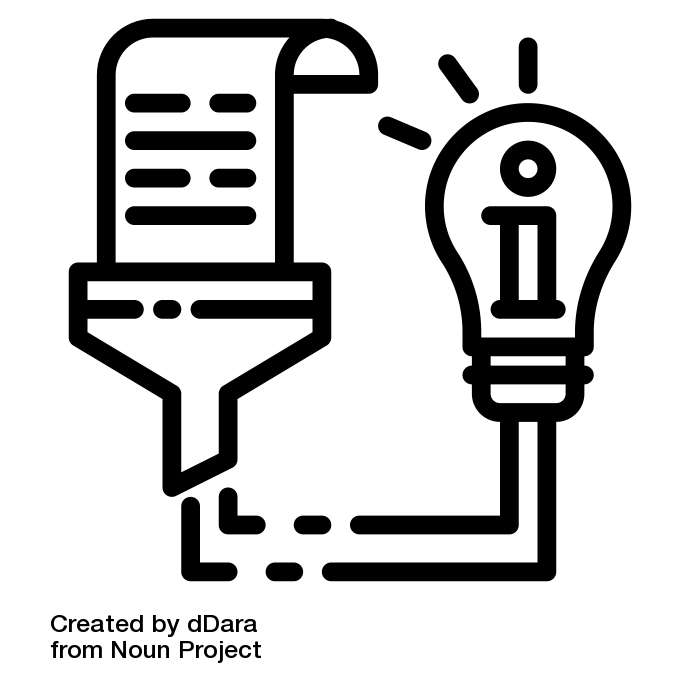
\includegraphics[width=0.9\textwidth]{symbols/symbol_tex_content}
				\end{wrapfigure}
				
				„Bei der Milchsäure handelt es sich um die 2-Hydroxypropansäure. Die L-(+)-Milchsäure entsteht in der Natur z.B. beim Gären von Milch und macht diese dann sauer.“
				\vspace{1.5cm}
			\end{tcolorbox}		

\vspace{0.3cm}
			\noindent \textbf{Auftrag: Zeichnen Sie Milchsäure in der Fischer-Projektion.}
			\begin{enumerate}
				\item Prüfen Sie ob es eine L/D-Milchsäure gibt und zeichnen Sie gegebenenfalls beide Enantiomere. 
    			\item Markieren Sie alle Chiralitätszentren.
			\end{enumerate} 

			\noindent \textbf{Auftrag: Erabeiten Sie sich die Hintergründe von links- bzw. rechtsdrehenden Substanzen.}
			\begin{enumerate}
			\item \textbf{Erklären} Sie den Begriff Optische Aktivität!
		    \item \textbf{Erklären} Sie die Funktionsweise eines Polarimeters!
		    \item \textbf{Erläutern} Sie wie man Enantiomere im Labor unterscheiden kann!
		    \item \textbf{Begründen} Sie, warum D(-)-Fructose nicht rechtsdrehend ist, obwohl der Vorsatz im Namen D für „rechts“ steht!
		    \item \textbf{Erklären} Sie den Begriff Racemat!
			\end{enumerate}

\vspace{0.3cm}
			\begin{tcolorbox}[enhanced,
				colback=white,
				colframe=darkgray,
				fonttitle=\sffamily\bfseries\large, 
				title=Eigenschaften der Enantiomere,  % search keyword::Informationstexte 
				attach boxed title to top left={xshift=3.2mm,yshift=-0.50mm},
				boxed title style={skin=enhancedfirst jigsaw,size=small,arc=1mm,bottom=-1mm,colframe=darkgray,height=0.75cm},
				colbacktitle=darkgray,
				drop lifted shadow]
				\begin{wrapfigure}{L}{0.15\textwidth}  
					\centering
					\vspace{-14pt}  % to align image with first line of text
					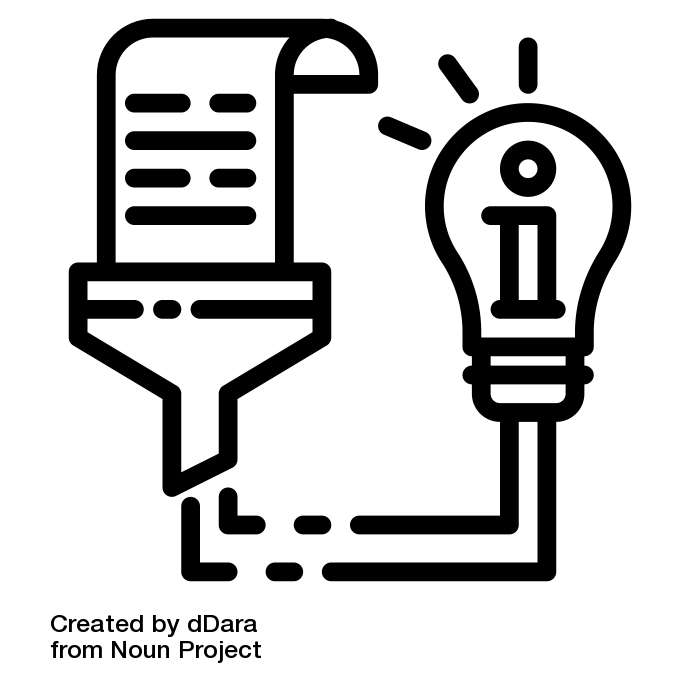
\includegraphics[width=0.9\textwidth]{symbols/symbol_tex_content}
				\end{wrapfigure}
				
				Aufgrund der strukturellen Verknüpfungen haben Enantiomere auch identische chemische und physikalische Eigenschaften (wie z.B. Schmelz- und Siedetemperatur). Es gibt jedoch 2 Ausnahmen. \newline
				Die erste betrifft die unterschiedliche Wechselwirkung mit anderen chiralen Molekülen, was Unterschiede in ihren physiologischen (pharmakologischen und toxikologischen) Wirkungen und ihren sensorischen Eigenschaften (Geruch, Pheromon-Wirkung) zur Folge hat. Der Duftstoff in Orangen, ein Enantiomer des Limonens, riecht nach Orangen, sein Spiegelbild dagegen nach Terpentin. \newline 
				Die andere Ausnahme betrifft die Wechselwirkungen mit linear polarisiertem Licht. Chirale Moleküle sind optisch aktiv, d.h dass diese Stoffe die Schwingungsebene des Lichts drehen. Man spricht daher auch von optischen Isomeren. Dadurch kann man optisch aktive Stoffe auch physikalisch mit einem Polarimeter untersuchen.\newline 
				Mit einem Polarimeter kann die optische Aktivität  einer Verbindung untersucht werden. Dazu misst man den Drehwinkel $\alpha$, d.h. den Winkel, um den die Schwingungsebene des linear polarisierten Lichts beim Durchgang durch die optisch aktive Lösung gedreht wird.
			\end{tcolorbox}			
			
			\begin{tcolorbox}[enhanced,
				colback=white,
				colframe=darkgray,
				fonttitle=\sffamily\bfseries\large, 
				title=Messung der Enantiomere,  % search keyword::Informationstexte 
				attach boxed title to top left={xshift=3.2mm,yshift=-0.50mm},
				boxed title style={skin=enhancedfirst jigsaw,size=small,arc=1mm,bottom=-1mm,colframe=darkgray,height=0.75cm},
				colbacktitle=darkgray,
				drop lifted shadow]
				\begin{wrapfigure}{L}{0.15\textwidth}  
					\centering
					\vspace{-14pt}  % to align image with first line of text
					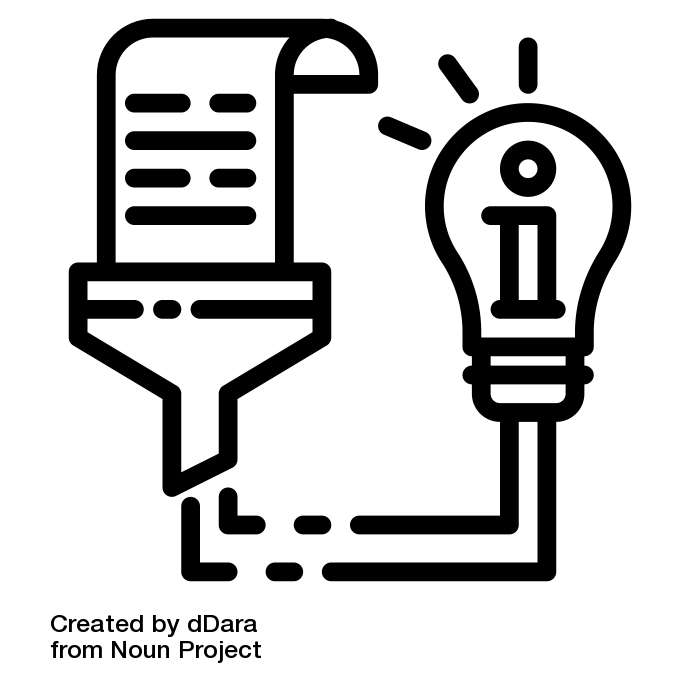
\includegraphics[width=0.9\textwidth]{symbols/symbol_tex_content}
				\end{wrapfigure}
				
				Mit einem Polarimeter kann die optische Aktivität  einer Verbindung untersucht werden. Dazu misst man den Drehwinkel $\alpha$, d.h. den Winkel, um den die Schwingungsebene des linear polarisierten Lichts beim Durchgang durch die optisch aktive Lösung gedreht wird.
				\begin{center}
					\includegraphics[width=0.5\textwidth]{images/polarisator}
				\end{center}
				Die Zeichen (+) und (-) geben die Änderung der Schwingungsrichtung des linear polarisierten Lichts an. (+) steht für (vom Beobachter aus) rechts, (-) für links herum. \newline 
				Bei einem 1:1 Gemisch beider Enantiomere hebt sich die Drehung auf. Ein solches Gemisch nennt man racemisches Gemisch oder Racemat. Enantiomere drehen die Ebene des polarisierten Lichts zwar in entgegengesetzte Richtungen, aber um den gleichen Betrag. So ist ein Racemat optisch inaktiv (+-). \newline
				Die Drehung im Polarimeter ist stoff- und konzentrationsabhängig sowie abhängig von der Länge des Polarimeters. Dadurch hat man eine Möglichkeit unbekannte Stoffe oder Konzentrationen in Lösungen mit dem Polarimeter zu untersuchen. \newline
				Die Formel dazu lautet: 
				\begin{center}
					$\alpha = \alpha_{sp} \cdot \beta \cdot l$
				\end{center}
				[$\alpha$ = gemessener Drehwinkel in ° // $\alpha_{sp}$ = spezifischer Drehwinkel in $\frac{°}{\frac{g}{ml} \cdot dm}$ // $\beta$ = Massen-Konzentration des Stoffs in $\frac{g}{ml}$ // l = Länge des Polarimeters (in dm)]
			\end{tcolorbox}

\vspace{0.3cm}
			\begin{tcolorbox}[enhanced,
				colback=white,
				colframe=darkgray,
				fonttitle=\sffamily\bfseries\large, 
				title=Wertetabelle für einige Stoffe,  % search keyword::Informationstexte 
				attach boxed title to top left={xshift=3.2mm,yshift=-0.50mm},
				boxed title style={skin=enhancedfirst jigsaw,size=small,arc=1mm,bottom=-1mm,colframe=darkgray,height=0.75cm},
				colbacktitle=darkgray,
				drop lifted shadow]
				\begin{wrapfigure}{L}{0.15\textwidth}  
					\centering
					\vspace{-14pt}  % to align image with first line of text
					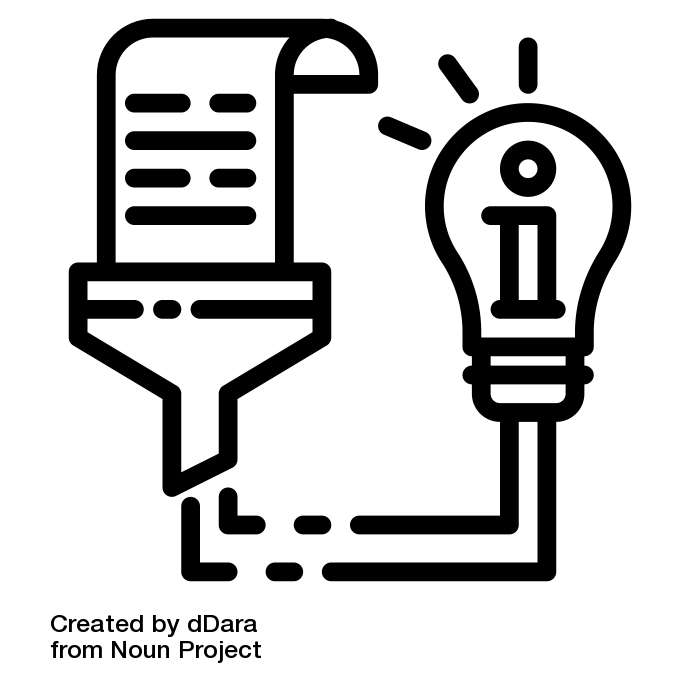
\includegraphics[width=0.9\textwidth]{symbols/symbol_tex_content}
				\end{wrapfigure}
				
				Einige Standardwerte für $\alpha_{sp}$: 
				\begin{center}
					\begin{tabular}{|c|c|}
						\hline
						Stoff & $\alpha_{sp}$ in $\frac{°}{\frac{g}{ml} \cdot dm}$ \\
						\hline
						D(+)-Glucose & +52,7 \\
						D(-)-Fructose & -92,4 \\
						D(+)-Galactose & +80,2 \\
						D(-)-Milchsäure & -3,8 \\
						Saccharose & +66,5 \\
						\hline
					\end{tabular}
				\end{center}
				
			\end{tcolorbox}
\vspace{0.3cm}

			\noindent \textbf{Auftrag: Wenden Sie ihr Wissen an!}
			\begin{enumerate}
			\item \textbf{Berechnen} Sie die Massenkonzentration $\beta$ einer Fructoselösung, deren Drehwinkel im Polarimeter mit $\alpha$ = -10° bestimmt wird. Die Messzelle des Polarimeters ist 10 cm lang. Achten Sie auf eine korrekte Einheitenrechnung!
    		\item \textbf{Erläutern} Sie die Bezeichnung L(+) auf unserem Joghurt aus dem Supermarkt. Gibt es auch linksdrehende Milchsäure? 
    		\item \textbf{Recherchieren} Sie im Internet, ob rechtsdrehende Milchsäure einen positiven Einfluss auf unseren Körper hat.	
    		\end{enumerate}
    		
    		\noindent \textbf{Auftrag: Kann man die optische Aktivität beim Bierbrauen nutzen?}
    		\begin{enumerate}
    		\item Lesen Sie den Text zur Stammwürze\footnote{Quelle:https://de.wikipedia.org/wiki/Stammwürze [Stand:25.8.2016]}.
    		 \item Aus der Stammwürze kann man über eine Formel den späteren Alkoholgehalt berechnen. Die Messung der Stammwürze erfolgt über die Dichte. Maltose ist aber auch optisch aktiv. Könnte ich dann nicht die Konzentration der Maltose über die optische Aktivität messen? Bewerten Sie die Eignung des Messverfahrens.
    		\end{enumerate}

\vspace{0.3cm}
			\begin{tcolorbox}[enhanced,
				colback=white,
				colframe=darkgray,
				fonttitle=\sffamily\bfseries\large, 
				title=Die Stammwürze,  % search keyword::Informationstexte 
				attach boxed title to top left={xshift=3.2mm,yshift=-0.50mm},
				boxed title style={skin=enhancedfirst jigsaw,size=small,arc=1mm,bottom=-1mm,colframe=darkgray,height=0.75cm},
				colbacktitle=darkgray,
				drop lifted shadow]
				\begin{wrapfigure}{L}{0.15\textwidth}  
					\centering
					\vspace{-14pt}  % to align image with first line of text
					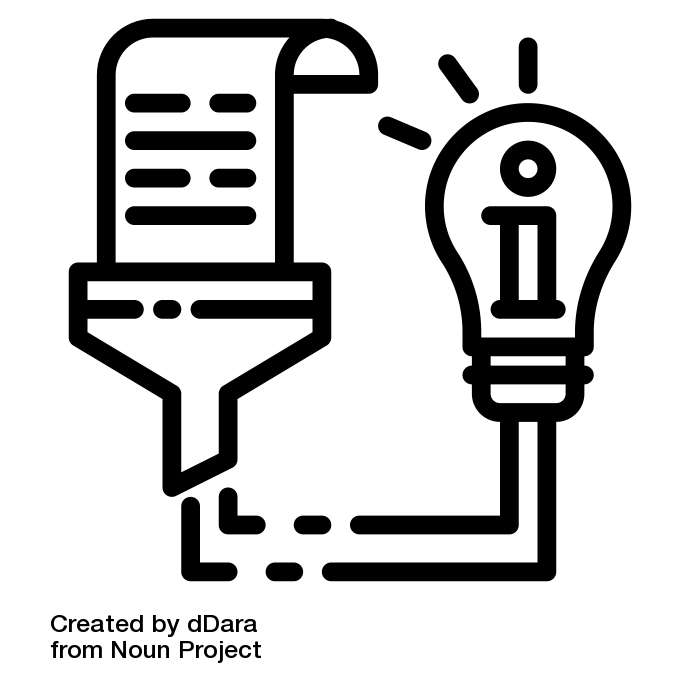
\includegraphics[width=0.9\textwidth]{symbols/symbol_tex_content}
				\end{wrapfigure}
				
				Die Stammwürze oder der Stammwürzgehalt ist eine entscheidende Messgröße beim Bierbrauen. Sie bezeichnet den Anteil der aus dem Malz und Hopfen im Wasser gelösten, nicht flüchtigen Stoffe vor der Gärung; es sind vor allem Malzzucker, Eiweiß, Vitamine und Aromastoffe. \newline
				Der Stammwürzegehalt ist der Haupteinflussfaktor für den späteren Alkoholgehalt und den Nährwert des fertigen Bieres. Die Stammwürze wird mit Hilfe der Hefe etwa jeweils zu einem Drittel in Alkohol und Kohlensäure vergoren; das letzte Drittel der Stammwürze ist unvergärbarer Restextrakt. \newline 
				Laut der Balling-Formel entstehen aus 2,0665g Extrakt bei der Gärung 1g Alkohol, 0,11g Hefe und 0,9565g \ch{CO2}.				
			\end{tcolorbox}

\vspace{0.3cm}			
			\begin{tcolorbox}[enhanced,
				colback=white,
				colframe=red,
				fonttitle=\sffamily\bfseries\large, 
				title=Für schnelle Schüler\_innen,  % search keyword::schnelle_Schüler
				attach boxed title to top left={xshift=3.2mm,yshift=-0.40mm},
				boxed title style={skin=enhancedfirst jigsaw,size=small,arc=1mm,bottom=-1mm,colframe=red,height=0.75cm},
				colbacktitle=red,
				drop lifted shadow]
				\begin{wrapfigure}{L}{0.15\textwidth}  
					\centering
					\vspace{-14pt}  % to align image with first line of text
					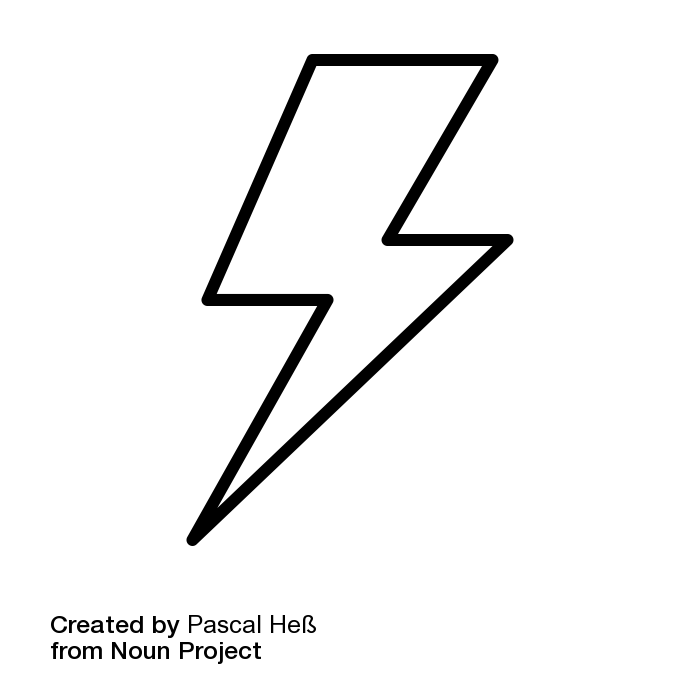
\includegraphics[width=0.8\textwidth]{symbols/symbol_tex_faststudents}
				\end{wrapfigure}
				
				\textbf{Recherchieren} Siewo Polarisationsfilter noch eingesetzt werden! Welchen Zweck erfüllen sie dabei?
				\newline
				Beim Bierbrauen stellt man den Zuckergehalt mit einer Spindel fest. \textbf{Recherchieren} Sie worum es sich dabei genau handelt und welches Prinzip dahinter steckt.
				
			\end{tcolorbox}

\newpage
	\section{Die HAYWORTH-Projektion}
	
		\textit{Bei der Messung der optischen Aktivität einer frischen Glucose-Lösung will sich der Drehwinkel nicht sofort einstellen, sondern verändert sich allmählich. Es scheint als wäre die Betrachtung der Glucose noch nicht an ihrem Ende angekommen.} \newline

		\begin{minipage}{0.7\textwidth}
			% *******************************
			% Übersicht Lernziele // Overview  
			% *******************************
			\noindent \textbf{Am Ende dieses Kapitels sollen Sie ... :}
			\begin{enumerate}
				\item ... die verschiedenen Konfigurationen der Glucose und Fructose erläutern können.
				\item ... die Auswirkungen auf die optische Aktivität erklären können.
				\item ... den Einfluss auf die Redoxeigenschaften erklären können.
			\end{enumerate}
			% *************************************************
			% empfohlene Vorgehensweise // recommended approach  
			% *************************************************
			% Lernende können selbst entscheiden, wie sie sich durch das Kapitel arbeiten
			% Lehrpersonen/Lernende können folgende Empfehlung aber nutzen
			\textbf{Vorgehensweise:}
			\begin{enumerate}
				\item Arbeiten Sie erst einmal allein.
				\item Bearbeiten Sie die Aufgaben in den Vorüberlegungen!
				\item Bearbeiten Sie alle Arbeitsaufträge.
				\item Führen Sie die Experimente in kleinen Gruppen durch.
			\end{enumerate}
			
		\end{minipage}
		\hspace{0.1\textwidth}
		% ***********************************
		% empfohlene Zeit // recommended time  
		% ***********************************
		% zeitliche Orientierung für Lernende und Lehrpersonen
		% Zeit sollte aber ungefährt eingehalten werden, damit Reihenplanung funktioniert
		\begin{minipage}{0.2\textwidth}
			\begin{tcolorbox}
				[enhanced,
				width=0.9\textwidth,
				colback=white,
				colframe=black,
				fonttitle=\sffamily\bfseries\large, 
				title=Zeit,  % search keyword::Zeit
				attach boxed title to top center={xshift=-0.0mm,yshift=-0.50mm},
				boxed title style={skin=enhancedfirst jigsaw,size=small,arc=1mm,bottom=-1mm,colframe=black,height=0.75cm},
				colbacktitle=black,
				drop lifted shadow]
				\centering
				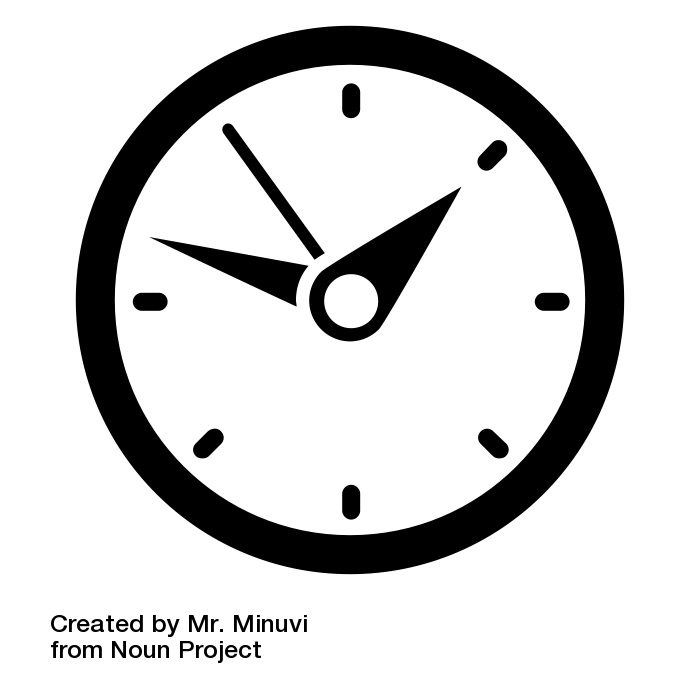
\includegraphics[width=0.9\textwidth]{symbols/symbol_tex_time}
				
				\begin{center}
					\textbf{90min} % Zeitangabe für Lernende // study time for students 
				\end{center}
			\end{tcolorbox}
		\end{minipage}

\vspace{0.3cm}
		% *********************************************
		% empfohlene Wiederholung // recommended review  
		% *********************************************
		\begin{tcolorbox}[enhanced,
			colback=white,
			colframe=orange!60!red,
			fonttitle=\sffamily\bfseries\large, 
			title=Vorüberlegung,  % search keyword::Wiederholung
			attach boxed title to top left={xshift=3.2mm,yshift=-0.50mm},
			boxed title style={skin=enhancedfirst jigsaw,size=small,arc=1mm,bottom=-1mm,colframe=orange!60!red,height=0.75cm},
			colbacktitle=orange!60!red,
			% sharp corners,
			drop lifted shadow]	
			\begin{wrapfigure}{L}{0.15\textwidth}  
				\centering
				\vspace{-14pt}  % to align image with first line of text
				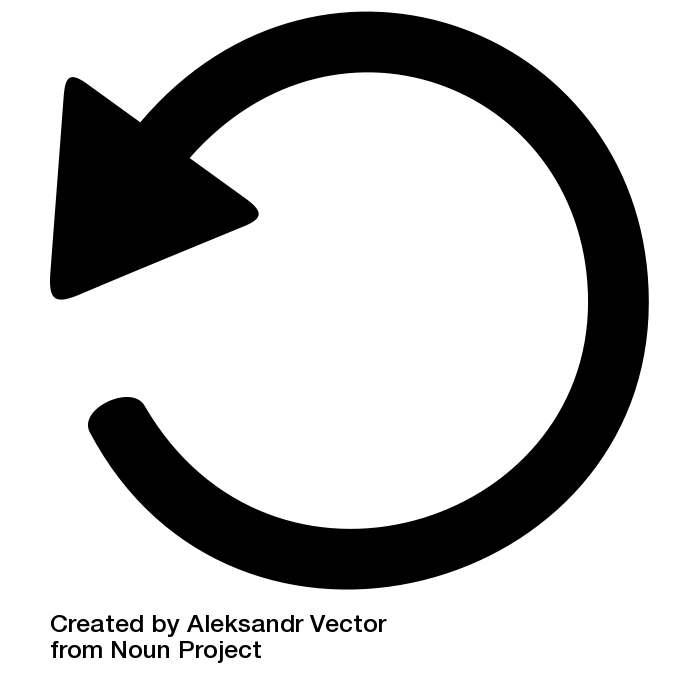
\includegraphics[width=0.9\textwidth]{symbols/symbol_tex_review}
			\end{wrapfigure}
			
			\textbf{Wiederholen} Sie den Begriff \textit{Isomerie}.
			\vspace{1.7cm}
		\end{tcolorbox}
		% Layout: Linie zum Abgrenzen
		\begin{center}
			\noindent\rule{18cm}{0.1pt}
		\end{center}
	% *********************************************
	% Ende Kapitelübersicht // End Chapter Overview
	% *********************************************				
\newpage

		\subsection{Optische Aktivität und Mutarotation}
		
			\textbf{Auftrag: Erläutern Sie die Mutarotation und ihre Folgen.}
			\begin{enumerate}
			   \item \textbf{Lesen} Sie den Text.
			   \item Nutzen Sie den \textbf{Molekülbaukasten} um die Beschreibung der Mutarotation nachzuvollziehen.
			   \item \textbf{Vervollständigen} Sie die unten stehende Gleichgewichtsreaktion! \textbf{Erklären} Sie warum zwei verschiedene Produkte entstehen können.
			   \item \textbf{Kennzeichnen} Sie in allen 3 Molekülen die asymmetrischen C-Atome. \textbf{Recherchieren und erklären} Sie warum es zu einer Änderung des Drehwinkels kommt.
			   \item \textbf{Vergleichen} Sie die Polysaccharide Stärke und Cellulose. \textbf{Erläutern} Sie die unterschiedlichen Strukturen.
			\end{enumerate}
			
			\begin{tcolorbox}[enhanced,
				colback=white,
				colframe=darkgray,
				fonttitle=\sffamily\bfseries\large, 
				title=Die Mutarotation,  % search keyword::Informationstexte 
				attach boxed title to top left={xshift=3.2mm,yshift=-0.50mm},
				boxed title style={skin=enhancedfirst jigsaw,size=small,arc=1mm,bottom=-1mm,colframe=darkgray,height=0.75cm},
				colbacktitle=darkgray,
				drop lifted shadow]
				\begin{wrapfigure}{L}{0.15\textwidth}  
					\centering
					\vspace{-14pt}  % to align image with first line of text
					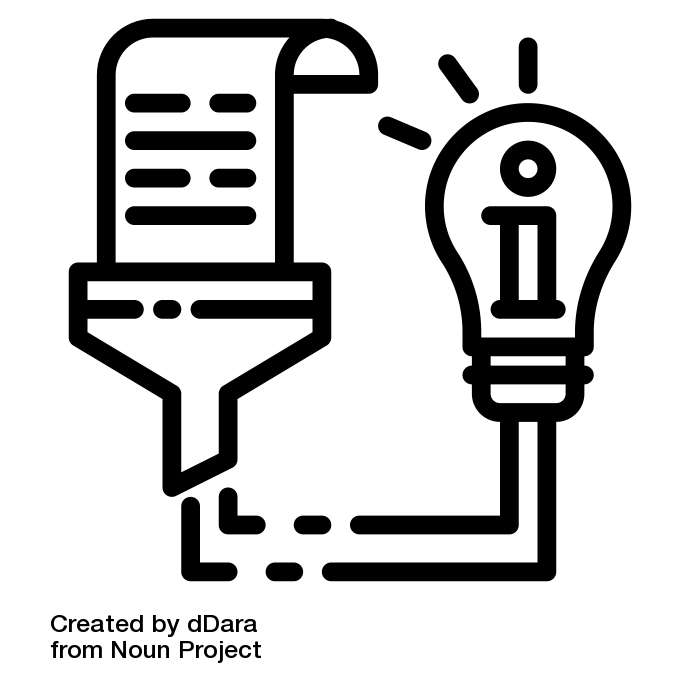
\includegraphics[width=0.9\textwidth]{symbols/symbol_tex_content}
				\end{wrapfigure}
				
				In wässrigen Lösungen liegen nur < 1\% der Glucose-Moleküle in der Kettenform vor. Moderne Strukturanalysen ergaben einen größeren Anteil an ringförmigen Strukturen. \newline 
				Die Ringform bildet sich aus der Kettenform durch die Reaktion der OH-Gruppe am C5-Atom mit der Aldehydgruppe am C1-Atom. Dabei handelt es sich um eine intramolekulare nucleophile Addition: Das negativ polarisierte Sauerstoff-Atom der Hydroxyl-Gruppe greift am positiv polarisierten C-Atom der Aldehydgruppe an. Dazu wechselt das Wasserstoffatom den Bindungspartner: es geht vom Sauerstoffatom der Hydroxylgruppe zum Sauerstoffatom der Aldehydgruppe und bildet dort eine Hydroxylgruppe. \newline
				\begin{center}
					\includegraphics[width=0.5\textwidth]{images/halbacetal}
				\end{center}
				Bei der Reaktion entsteht ein sechsgliedriger Ring. 6-Ring-Zucker heißen Pyranosen.  Allgemein bezeichnet man das Produkt der Reaktion zwischen einem Aldehyd und einem Alkohol als Halbacetal. Im Halbacetal-Molekül ist das C-Atom, das zuvor zur Aldehyd-Gruppe gehörte, zugleich verethert (-OR) und mit einer Hydroxy-Gruppe (-OH) verbunden. Wegen der beiden elektronegativen Substituenten ist dieses C-Atom besonders reaktiv. Bei der Reaktion mit anderen Monosacchariden wird ein Wassermolekül abgespalten. Es handelt sich um eine Kondensationsreaktion. Zuckeracetale werden allgemein als Glykoside bezeichnet. Das ursprüngliche Carbonyl-C-Atom (das C-Atom der Aldehyd-Gruppe) nennt man glykosidisches C-Atom, die von diesem Atom zum Alkohol ausgehende Bindung (C-OR) heißt glykosidische Bindung. \newline
				Zur Darstellung der Ringe nutzt man die Haworth-Projektion.		
				\begin{center}
					\includegraphics[width=0.75\textwidth]{images/hayworth_glucose}
				\end{center}		
			\end{tcolorbox}
			
		\subsection{Die Ringe der Fructose}
			
			\textbf{Auftrag: Stellen Sie die Fructose in der Haworth-Projektion dar.}
			\begin{enumerate}
				\item Nutzen Sie die Informationen aus dem Text und den Molekülbaukasten, um die entsprechenden Moleküle zu \textbf{zeichnen}.
			    \item Anomere sind spezielle Formen der Isomere. Sie unterscheiden sich durch die Konfiguration – die räumliche Anordnung von Atomen oder Molekülen – am anomeren Zentrum oder C-Atom. \textbf{Kennzeichnen} Sie die jeweiligen anomeren Zentren. \textbf{Erklären} Sie wie man sie unterscheidet. 
			\end{enumerate} 
			
			\begin{tcolorbox}[enhanced,
				colback=white,
				colframe=darkgray,
				fonttitle=\sffamily\bfseries\large, 
				title=Die Ringe der Fructose,  % search keyword::Informationstexte 
				attach boxed title to top left={xshift=3.2mm,yshift=-0.50mm},
				boxed title style={skin=enhancedfirst jigsaw,size=small,arc=1mm,bottom=-1mm,colframe=darkgray,height=0.75cm},
				colbacktitle=darkgray,
				drop lifted shadow]
				\begin{wrapfigure}{L}{0.15\textwidth}  
					\centering
					\vspace{-14pt}  % to align image with first line of text
					\includegraphics[width=0.9\textwidth]{symbols/symbol_tex_content}
				\end{wrapfigure}
				
				Aus der D-Frucotse lassen sich 4 verschiedene Ringe bilden. Dabei muss man beachten, dass bei der Fructose keine Aldehydgruppe sondern eine Ketogruppe vorliegt. \newline
				Es bilden sich entweder Fünfringe, sogenannte Furanosen, oder Sechsringe, auch Pyranosen genannt. Bei der Fructofuranose findet eine Ringbindung zwischen dem C2 und C5 Atom statt. Bei den Pyranosen zwischen C2 und C6. Darüber hinaus gibt es auch hier jeweils ein $\alpha$ und ein $\beta$-Anomer.		
			\end{tcolorbox}			
			
\newpage
	\section{Die Redoxeigenschaften der Zucker}
	
		\textit{Um Mono- und Disaccharide nachzuweisen, kann man nicht immer auf technische Hilfsmittel zurückgreifen. Manchmal reichen auch schon einfache Experimente. Diese Nachweise sollen Sie in diesem Kapitel durchführen.} \newline

		\begin{minipage}{0.7\textwidth}
			% *******************************
			% Übersicht Lernziele // Overview  
			% *******************************
			\noindent \textbf{Am Ende dieses Kapitels sollen Sie ... :}
			\begin{enumerate}
				\item ... die Begriffe \textit{Oxidation}, \textit{Reduktion} und \textit{Redoxreaktion} erklären können.
				\item ... mit Hilfe der Redoxreaktionen die verschiedenen Reaktionen der Zucker erklären können.
			\end{enumerate}
			% *************************************************
			% empfohlene Vorgehensweise // recommended approach  
			% *************************************************
			% Lernende können selbst entscheiden, wie sie sich durch das Kapitel arbeiten
			% Lehrpersonen/Lernende können folgende Empfehlung aber nutzen
			\textbf{Vorgehensweise:}
			\begin{enumerate}
				\item Arbeiten Sie erst einmal allein.
				\item Bearbeiten Sie die Aufgaben in den Vorüberlegungen!
				\item Bearbeiten Sie alle Arbeitsaufträge.
				\item Führen Sie die Experimente in kleinen Gruppen durch.
			\end{enumerate}
			
		\end{minipage}
		\hspace{0.1\textwidth}
		% ***********************************
		% empfohlene Zeit // recommended time  
		% ***********************************
		% zeitliche Orientierung für Lernende und Lehrpersonen
		% Zeit sollte aber ungefährt eingehalten werden, damit Reihenplanung funktioniert
		\begin{minipage}{0.2\textwidth}
			\begin{tcolorbox}
				[enhanced,
				width=0.9\textwidth,
				colback=white,
				colframe=black,
				fonttitle=\sffamily\bfseries\large, 
				title=Zeit,  % search keyword::Zeit
				attach boxed title to top center={xshift=-0.0mm,yshift=-0.50mm},
				boxed title style={skin=enhancedfirst jigsaw,size=small,arc=1mm,bottom=-1mm,colframe=black,height=0.75cm},
				colbacktitle=black,
				drop lifted shadow]
				\centering
				\includegraphics[width=0.9\textwidth]{symbols/symbol_tex_time}
				
				\begin{center}
					\textbf{90min} % Zeitangabe für Lernende // study time for students 
				\end{center}
			\end{tcolorbox}
		\end{minipage}

\vspace{0.3cm}
		% *********************************************
		% empfohlene Wiederholung // recommended review  
		% *********************************************
		\begin{tcolorbox}[enhanced,
			colback=white,
			colframe=orange!60!red,
			fonttitle=\sffamily\bfseries\large, 
			title=Vorüberlegung,  % search keyword::Wiederholung
			attach boxed title to top left={xshift=3.2mm,yshift=-0.50mm},
			boxed title style={skin=enhancedfirst jigsaw,size=small,arc=1mm,bottom=-1mm,colframe=orange!60!red,height=0.75cm},
			colbacktitle=orange!60!red,
			% sharp corners,
			drop lifted shadow]	
			\begin{wrapfigure}{L}{0.15\textwidth}  
				\centering
				\vspace{-14pt}  % to align image with first line of text
				\includegraphics[width=0.9\textwidth]{symbols/symbol_tex_review}
			\end{wrapfigure}
			
			\textbf{Erklären} Sie den Begriff Redoxreaktion so wie Sie ihn bisher kennengelernt haben! \newline
			\textbf{Wiederholen oder recherchieren} Sie das Konzept der Oxidationszahlen. \newline
			\textbf{Nennen} Sie die Redoxzahlen in der Aldehydgruppe und der Carboxlygruppe!
			\vspace{1cm}			
		\end{tcolorbox}
		% Layout: Linie zum Abgrenzen
		\begin{center}
			\noindent\rule{18cm}{0.1pt}
		\end{center}
	% *********************************************
	% Ende Kapitelübersicht // End Chapter Overview
	% *********************************************				

\newpage
		\subsection{Die Redoxreaktion}
			\textbf{Auftrag: Bearbeiten Sie die gegebenen Aufgaben und erklären Sie damit den Begriff Redoxreaktion!}
			\begin{enumerate}
			    \item \textbf{Formulieren} Sie die ausgeglichene Reaktionsgleichung für die Verbrennung von Magnesium!
			    \item \textbf{Kennzeichnen} Sie mit Hilfe von Pfeilen wo die Oxidation verläuft und wo die Reduktion verläuft!
			    \item Schreiben Sie alle Redoxzahlen über die jeweiligen Edukte und Produkte! \textbf{Erklären} Sie mit Hilfe von Elektronen die Änderungen der Rexoxzahlen!
			    \item \textbf{Erläutern} Sie mit Hilfe der Gleichung, den Pfeilen und den Redoxzahlen die Begriffe Oxidation und Reduktion in Hinblick auf die Wanderung der Elektronen. 
			    \item \textbf{Erklären} Sie den Begriff Redoxreaktion!
			\end{enumerate}


		\subsection{Die Redoxeigenschaften der Mono- und Disaccharide}
			\textbf{Auftrag: Untersuchen Sie die Redoxeigenschaften der Mono- und Disaccharide.}
			\begin{enumerate}
				\item Führen Sie die Experimente in kleinen Gruppen durch.
				\item Schreiben Sie ein \textbf{ausführliches Protokoll}. Sie werden bewertet! 
				\item Beantworten Sie innerhalb Ihrer Auswertung \underline{auch} die vorgegebenen Fragen.
				\item \textbf{Liste der Experimente:}
				\begin{itemize}
					\item Fehling-Probe
					\item Tollensprobe (auch Silberspiegelprobe)
				\end{itemize}
				\item \textbf{Liste der zu untersuchenden Zucker:}
				\begin{itemize}
					\item Glucose
					\item Fructose
					\item Maltose
					\item Saccharose
				\end{itemize}
				\item \textbf{Fragen für die Auswertung:}
				\begin{itemize}
					\item \textbf{Erläutern} Sie die chemischen Hintergründe ihrer Beobachtungen. Beziehen Sie sich dabei immer auf das Konzept der Redoxreaktion und die funktionellen Gruppen der Moleküle.
					\item \textbf{Vergleichen} Sie die Redoxeigenschaften von Mono- und Disacchariden.
					\item \textbf{Lesen} Sie die unten gegebenen Informationen zu Tollensprobe. \textbf{Erklären} Sie wie die Informationen von Wikipedia im Widerspruch zu unseren experimentellen Ergebnissen stehen. 
			        \item \textbf{Erläutern} Sie, warum Fructose auch bei der Silberspiegelprobe positive Ergebnisse erzeugt.
			        \item \textbf{Erklären} Sie den Begriff Tautomerie! \textbf{Vergleichen} Sie dazu „normale“ Isomere zu Isomeren, die sich durch Tautomerie gebildet haben.
			        \item \textbf{Erläutern} Sie anhand von Molekülformeln die Keto-Enol-Tautomerie!
			        \item \textbf{Lesen} Sie den unten gegebenen Text zur Schiffschen Probe. \textbf{Erläutern} Sie die fehlenden Redoxeigenschaften der D-Glucose.
				\end{itemize}
			\end{enumerate}

\vspace{0.3cm}
			\begin{tcolorbox}[enhanced,
				colback=white,
				colframe=darkgray,
				fonttitle=\sffamily\bfseries\large, 
				title=Die Tollensprobe,  % search keyword::Informationstexte 
				attach boxed title to top left={xshift=3.2mm,yshift=-0.50mm},
				boxed title style={skin=enhancedfirst jigsaw,size=small,arc=1mm,bottom=-1mm,colframe=darkgray,height=0.75cm},
				colbacktitle=darkgray,
				drop lifted shadow]
				\begin{wrapfigure}{L}{0.15\textwidth}  
					\centering
					\vspace{-14pt}  % to align image with first line of text
					\includegraphics[width=0.9\textwidth]{symbols/symbol_tex_content}
				\end{wrapfigure}
				
				Die Tollensprobe (benannt nach dem Agrikulturchemiker Bernhard Tollens) oder Silberspiegelprobe ist ein Nachweis für Aldehyde [...]\footnote{Quelle: Wikipedia [Stand: 08.2014]}. 
				\vspace{1.0cm}		
			\end{tcolorbox}

\vspace{0.3cm}
			\begin{tcolorbox}[enhanced,
				colback=white,
				colframe=darkgray,
				fonttitle=\sffamily\bfseries\large, 
				title=Die Schiff'sche Probe,  % search keyword::Informationstexte 
				attach boxed title to top left={xshift=3.2mm,yshift=-0.50mm},
				boxed title style={skin=enhancedfirst jigsaw,size=small,arc=1mm,bottom=-1mm,colframe=darkgray,height=0.75cm},
				colbacktitle=darkgray,
				drop lifted shadow]
				\begin{wrapfigure}{L}{0.15\textwidth}  
					\centering
					\vspace{-14pt}  % to align image with first line of text
					\includegraphics[width=0.9\textwidth]{symbols/symbol_tex_content}
				\end{wrapfigure}
				
				Die Schiff'sche Probe ist eine nach ihrem Entdecker Hugo Schiff benannte chemische Reaktion, die zum Nachweis von Aldehyden genutzt wird. Bei der schiffschen Probe wird die farblose Fuchsinschweflige Säure (Schiffsches Reagenz) durch Spuren von Aldehyden rosa bis violett gefärbt. \newline
				Die Reaktion verläuft nicht mit Zuckern.\footnote{Quelle: Wikipedia [Stand 08.2014]}. 
				\vspace{0.1cm}		
			\end{tcolorbox}	


\newpage

				
				% ***** start copy here *********************************************************
				% *******************************************************************************
				%            __ _           _   _                        _                _   
				%  _ __ ___ / _| | ___  ___| |_(_) ___  _ __         ___| |__   __ _ _ __| |_ 
				% | '__/ _ \ |_| |/ _ \/ __| __| |/ _ \| '_ \ _____ / __| '_ \ / _` | '__| __|
				% | | |  __/  _| |  __/ (__| |_| | (_) | | | |_____| (__| | | | (_| | |  | |_ 
				% |_|  \___|_| |_|\___|\___|\__|_|\___/|_| |_|      \___|_| |_|\__,_|_|   \__|
				%                                                                            
				%
				
				\vspace{0.3cm}
				\begin{center}
					\begin{tcolorbox}[enhanced,
						width=0.75\textwidth,
						colback=white,
						colframe=darkgray,
						fonttitle=\sffamily\bfseries\large, 
						title=Kurzreflexion,  % search keyword::Informationstexte 
						attach boxed title to top left={xshift=3.2mm,yshift=-0.50mm},
						boxed title style={skin=enhancedfirst jigsaw,size=small,arc=1mm,bottom=-1mm,colframe=darkgray,height=0.75cm},
						colbacktitle=darkgray,
						drop lifted shadow]
						
						% \begin{figure}[htbp]  % not good in ecolorbox
						\textbf{Auftrag: Bewerten Sie Ihre Arbeit in der letzten Einheit selbst.} \newline
						\begin{center}
							\begin{tikzpicture}[scale=1]
								\path (0:0cm) coordinate (O); % define coordinate for origin
								
								% draw the spiderweb
								\foreach \X in {1,...,\D}{
									\draw (\X*\A:0) -- (\X*\A:\R);
								}
								
								\foreach \Y in {0,...,\U}{
									\foreach \X in {1,...,\D}{
								\path (\X*\A:\Y*\R/\U) coordinate (D\X-\Y);
								\fill (D\X-\Y) circle (1pt);
									}
									\draw [opacity=0.3] (0:\Y*\R/\U) \foreach \X in {1,...,\D}{
										-- (\X*\A:\Y*\R/\U)
									} -- cycle;
								}
								
								% define labels for each dimension axis (names config option)
								\path (1*\A:\L) node (L1) {\tiny Verständnis};
								\path (2*\A:\L) node (L2) {\tiny alle Aufgaben gelöst};
								\path (3*\A:\L) node (L3) {\tiny Zeit effektiv genutz};
								\path (4*\A:\L) node (L4) {\tiny Einzelarbeit};
								\path (5*\A:\L) node (L5) {\tiny Gruppenarbeit};
							
							\end{tikzpicture}
							% \caption{Diagramm Slebstreflexion}
							% \caption{Spiderweb Diagram (\D~Dimensions, \U-Notch Scale, 3 Samples)}
							% \label{fig:spiderweb}
							% \end{figure} 
						\end{center}
						\textbf{{\Large Was können Sie in der nächsten Stunde verbessern?}}
						\begin{center}
							%\vspace{1.1cm}
							\noindent\rule{12cm}{0.2pt}
							\vspace{1.1cm}
							\noindent\rule{12cm}{0.1pt}
							\vspace{1.1cm}
							\noindent\rule{12cm}{0.1pt}
							\vspace{1.1cm}
							\noindent\rule{12cm}{0.1pt}
							\vspace{1.1cm}
							\noindent\rule{12cm}{0.1pt}
							\vspace{1.1cm}
							\noindent\rule{12cm}{0.1pt}
							\vspace{1.1cm}
							\noindent\rule{12cm}{0.1pt}
							\vspace{1.1cm}
							\noindent\rule{12cm}{0.1pt}
						\end{center}
					\end{tcolorbox}
				\end{center}
								
				% *******************************************************************************
				% ***** end copy here ***********************************************************

\newpage

	\part{Der Aufbau der Polypeptide (Eiweiße)}
	
	\section{Die Struktur der Aminosäure}
	
		\textit{Nachdem Sie nun die Grundbausteine der Saccharide ausführlich bearbeitet haben, sollen Sie sich nun mit den Grundbausteinen der zweiten wichtigen Gruppe der Bio-Polymere beschäftigen. Wie sind die Proteine nun genau aufgebaut? Welche Grundbausteine gibt es? Wie sind sie verbunden? Und welche Eigenschaften ergeben sich daraus?} \newline
	
		\begin{minipage}{0.7\textwidth}
			% *******************************
			% Übersicht Lernziele // Overview  
			% *******************************
			\noindent \textbf{Am Ende dieses Kapitels sollen Sie ... :}
			\begin{enumerate}
				\item ... die grundlegende Struktur der Aminosäuren experimentell erarbeitet haben.
			\end{enumerate}
			% *************************************************
			% empfohlene Vorgehensweise // recommended approach  
			% *************************************************
			% Lernende können selbst entscheiden, wie sie sich durch das Kapitel arbeiten
			% Lehrpersonen/Lernende können folgende Empfehlung aber nutzen
			\textbf{Vorgehensweise:}
			\begin{enumerate}
				\item Bearbeiten Sie die Aufgaben in den Vorüberlegungen!
				\item Führen Sie die Experimente in kleinen Gruppen durch.
				\item Bearbeiten Sie alle Arbeitsaufträge.
			\end{enumerate}
			
		\end{minipage}
		\hspace{0.1\textwidth}
		% ***********************************
		% empfohlene Zeit // recommended time  
		% ***********************************
		% zeitliche Orientierung für Lernende und Lehrpersonen
		% Zeit sollte aber ungefährt eingehalten werden, damit Reihenplanung funktioniert
		\begin{minipage}{0.2\textwidth}
			\begin{tcolorbox}
				[enhanced,
				width=0.9\textwidth,
				colback=white,
				colframe=black,
				fonttitle=\sffamily\bfseries\large, 
				title=Zeit,  % search keyword::Zeit
				attach boxed title to top center={xshift=-0.0mm,yshift=-0.50mm},
				boxed title style={skin=enhancedfirst jigsaw,size=small,arc=1mm,bottom=-1mm,colframe=black,height=0.75cm},
				colbacktitle=black,
				drop lifted shadow]
				\centering
				\includegraphics[width=0.9\textwidth]{symbols/symbol_tex_time}
				
				\begin{center}
					\textbf{90min} % Zeitangabe für Lernende // study time for students 
				\end{center}
			\end{tcolorbox}
		\end{minipage}

\vspace{0.3cm}
		% *********************************************
		% empfohlene Wiederholung // recommended review  
		% *********************************************
		\begin{tcolorbox}[enhanced,
			colback=white,
			colframe=orange!60!red,
			fonttitle=\sffamily\bfseries\large, 
			title=Vorüberlegung,  % search keyword::Wiederholung
			attach boxed title to top left={xshift=3.2mm,yshift=-0.50mm},
			boxed title style={skin=enhancedfirst jigsaw,size=small,arc=1mm,bottom=-1mm,colframe=orange!60!red,height=0.75cm},
			colbacktitle=orange!60!red,
			% sharp corners,
			drop lifted shadow]	
			\begin{wrapfigure}{L}{0.15\textwidth}  
				\centering
				\vspace{-14pt}  % to align image with first line of text
				\includegraphics[width=0.9\textwidth]{symbols/symbol_tex_review}
			\end{wrapfigure}
			
			\textbf{Beschreiben} Sie Experimente, mit denen Sie Wasser und Kohlenstoffdioxid nachweisen können. \newline
			\vspace{1cm}
			
		\end{tcolorbox}
		% Layout: Linie zum Abgrenzen
		\begin{center}
			\noindent\rule{18cm}{0.1pt}
		\end{center}
	% *********************************************
	% Ende Kapitelübersicht // End Chapter Overview
	% *********************************************				

\newpage
	
		\subsection{Elementaranalyse von Glycin}
		
			\textbf{Auftrag: Ermitteln Sie experimentell die Elemente aus denen sich die Aminosäure Glycin zusammensetzt.}
			
			\begin{enumerate}
				\item Schreiben Sie ein \textbf{Protokoll}.
	    		\item Erstellen Sie eine \textbf{Arbeitshypothese} zu den enthaltenen Elementen, basierend auf Ihrem Vorwissen. \textbf{Begründen} Sie kurz.
	    		\item \textbf{Recherchieren} Sie zielführende Durchführungen für die Nachweise. Nutzen Sie gegebenenfalls die Hilfen der Lehrkraft. (Achtung: Falls Sie Watesmo-Papier nutzen sollen, müssen Sie auf weißes Kupfersulfat ausweichen. Dies können Sie durch die Erhitzung von blauem Kupfersulfat herstellen.)
	    		\item Für ihre \textbf{Auswertung}:
	        	\begin{itemize}
	        		\item Werten Sie ihre Beobachtungen detailliert aus. Bewerten Sie ihre Hypothese und erstellen Sie eine Fehlerbetrachtung. 
	        		\item Nutzen Sie in der Auswertung die korrekten chemischen Formeln sowie Wort- und Formelgleichungen (bei den Nachweisen).
	        		\item Recherchieren Sie die Strukturformel vom Glycin.
	        		\item Erklären Sie, welches Element nicht in der Elementaranalyse nachgewiesen wurde. Recherchieren Sie Nachweismöglichkeiten.
	        		\item Nennen Sie Beispiele für weitere Aminosäuren und deren Bedeutung.
				\end{itemize}
			\end{enumerate}

\newpage
	\section{Die Eigenschaften der Aminosäure}
	
		\textit{Ähnlich wie bei den Monosacchariden gibt es auch bei den Aminosäuren mehrere Vertreter. Die wichtigsten sollen Sie in diesem Kapitel kennenlernen. Dabei ist es wichtig eine Einteilung der Aminosäuren vorzunehmen.} \newline
	
		\begin{minipage}{0.7\textwidth}
			% *******************************
			% Übersicht Lernziele // Overview  
			% *******************************
			\noindent \textbf{Am Ende dieses Kapitels sollen Sie ... :}
			\begin{enumerate}
				\item ... die zwanzig wichtigsten Aminosäuren bzgl. ihrer Eigenschaften analysieren und einteilen können.
			\end{enumerate}
			% *************************************************
			% empfohlene Vorgehensweise // recommended approach  
			% *************************************************
			% Lernende können selbst entscheiden, wie sie sich durch das Kapitel arbeiten
			% Lehrpersonen/Lernende können folgende Empfehlung aber nutzen
			\textbf{Vorgehensweise:}
			\begin{enumerate}
				\item Bearbeiten Sie die Aufgaben erst einmal allein.
				\item Vergleichen Sie ihre Ergebnisse in der Gruppe.
				\item Bearbeiten Sie alle Arbeitsaufträge.
			\end{enumerate}
			
		\end{minipage}
		\hspace{0.1\textwidth}
		% ***********************************
		% empfohlene Zeit // recommended time  
		% ***********************************
		% zeitliche Orientierung für Lernende und Lehrpersonen
		% Zeit sollte aber ungefährt eingehalten werden, damit Reihenplanung funktioniert
		\begin{minipage}{0.2\textwidth}
			\begin{tcolorbox}
				[enhanced,
				width=0.9\textwidth,
				colback=white,
				colframe=black,
				fonttitle=\sffamily\bfseries\large, 
				title=Zeit,  % search keyword::Zeit
				attach boxed title to top center={xshift=-0.0mm,yshift=-0.50mm},
				boxed title style={skin=enhancedfirst jigsaw,size=small,arc=1mm,bottom=-1mm,colframe=black,height=0.75cm},
				colbacktitle=black,
				drop lifted shadow]
				\centering
				\includegraphics[width=0.9\textwidth]{symbols/symbol_tex_time}
				
				\begin{center}
					\textbf{45min} % Zeitangabe für Lernende // study time for students 
				\end{center}
			\end{tcolorbox}
		\end{minipage}

\vspace{0.3cm}
		% *********************************************
		% empfohlene Wiederholung // recommended review  
		% *********************************************
		\begin{tcolorbox}[enhanced,
			colback=white,
			colframe=orange!60!red,
			fonttitle=\sffamily\bfseries\large, 
			title=Vorüberlegung,  % search keyword::Wiederholung
			attach boxed title to top left={xshift=3.2mm,yshift=-0.50mm},
			boxed title style={skin=enhancedfirst jigsaw,size=small,arc=1mm,bottom=-1mm,colframe=orange!60!red,height=0.75cm},
			colbacktitle=orange!60!red,
			% sharp corners,
			drop lifted shadow]	
			\begin{wrapfigure}{L}{0.15\textwidth}  
				\centering
				\vspace{-14pt}  % to align image with first line of text
				\includegraphics[width=0.9\textwidth]{symbols/symbol_tex_review}
			\end{wrapfigure}
			
			    \textbf{Wiederholen Sie die folgenden chemischen Basiskonzepte:} \newline
			    $\bullet$ sauer und basisch \newline
			    $\bullet$ polar und unpolar
			\vspace{1cm}			
		\end{tcolorbox}
		% Layout: Linie zum Abgrenzen
		\begin{center}
			\noindent\rule{18cm}{0.1pt}
		\end{center}
	% *********************************************
	% Ende Kapitelübersicht // End Chapter Overview
	% *********************************************				

\newpage
		\subsection{Einteilung der Aminosäuren aufgrund spezifischer Eigenschaften}
		
			\textbf{Auftrag: Sortieren Sie die 20 Aminosäuren!}
			\begin{enumerate}
				\item Nutzen Sie die folgenden Kategorien: polar, unpolar, sauer und basisch.
			    \item \textbf{Erläutern} Sie die Eigenschaften anhand selbstgewählter Aminosäuren. Recherchieren Sie gegebenenfalls in der Literatur oder online.
			    \item \textbf{Bewerten} Sie die folgende Aussage: „Alle Aminosäuren sind optisch aktiv!“
			    \item \textbf{Erläutern} Sie, warum es sich bei Aminosäuren um Ampholyte handelt.
			    \item \textbf{Erklären} Sie die biologische Bedeutung der Aminosäuren für den Menschen.
			    \item \textbf{Erklären} Sie was essentielle Aminosäuren sind.
			\end{enumerate} 
			
			\begin{center}
				\includegraphics{images/table_aminoacids}
			\end{center}
			
\newpage
	\section{Von der Aminosäure zum Peptid}
	
		\textit{Aminosäuren sind der Monomerbaustein der Protoeine. Aber wie genau entsteht aus einzelnen Aminosäuren nun Proteine? Und welchen Einfluss hat die Zusammensetzung auf das Protein-Polymer (Polypeptid)?} \newline
	
		\begin{minipage}{0.7\textwidth}
			% *******************************
			% Übersicht Lernziele // Overview  
			% *******************************
			\noindent \textbf{Am Ende dieses Kapitels sollen Sie ... :}
			\begin{enumerate}
				\item ... die Bindung zwischen den Aminosäuren erklären können.
				\item ... die Strukturen die Polypeptide erklären können.
			\end{enumerate}
			% *************************************************
			% empfohlene Vorgehensweise // recommended approach  
			% *************************************************
			% Lernende können selbst entscheiden, wie sie sich durch das Kapitel arbeiten
			% Lehrpersonen/Lernende können folgende Empfehlung aber nutzen
			\textbf{Vorgehensweise:}
			\begin{enumerate}
				\item Bearbeiten Sie die Aufgaben erst einmal allein.
				\item Vergleichen Sie ihre Ergebnisse in der Gruppe.
				\item Bearbeiten Sie alle Arbeitsaufträge.
			\end{enumerate}
			
		\end{minipage}
		\hspace{0.1\textwidth}
		% ***********************************
		% empfohlene Zeit // recommended time  
		% ***********************************
		% zeitliche Orientierung für Lernende und Lehrpersonen
		% Zeit sollte aber ungefährt eingehalten werden, damit Reihenplanung funktioniert
		\begin{minipage}{0.2\textwidth}
			\begin{tcolorbox}
				[enhanced,
				width=0.9\textwidth,
				colback=white,
				colframe=black,
				fonttitle=\sffamily\bfseries\large, 
				title=Zeit,  % search keyword::Zeit
				attach boxed title to top center={xshift=-0.0mm,yshift=-0.50mm},
				boxed title style={skin=enhancedfirst jigsaw,size=small,arc=1mm,bottom=-1mm,colframe=black,height=0.75cm},
				colbacktitle=black,
				drop lifted shadow]
				\centering
				\includegraphics[width=0.9\textwidth]{symbols/symbol_tex_time}
				
				\begin{center}
					\textbf{45min} % Zeitangabe für Lernende // study time for students 
				\end{center}
			\end{tcolorbox}
		\end{minipage}

\vspace{0.3cm}
		% *********************************************
		% empfohlene Wiederholung // recommended review  
		% *********************************************
		\begin{tcolorbox}[enhanced,
			colback=white,
			colframe=orange!60!red,
			fonttitle=\sffamily\bfseries\large, 
			title=Vorüberlegung,  % search keyword::Wiederholung
			attach boxed title to top left={xshift=3.2mm,yshift=-0.50mm},
			boxed title style={skin=enhancedfirst jigsaw,size=small,arc=1mm,bottom=-1mm,colframe=orange!60!red,height=0.75cm},
			colbacktitle=orange!60!red,
			% sharp corners,
			drop lifted shadow]	
			\begin{wrapfigure}{L}{0.15\textwidth}  
				\centering
				\vspace{-14pt}  % to align image with first line of text
				\includegraphics[width=0.9\textwidth]{symbols/symbol_tex_review}
			\end{wrapfigure}
			
			    \textbf{Wiederholen Sie die folgenden chemischen Basiskonzepte:} \newline
			    $\bullet$ Wasserstoffbrückenbindungen \newline
			    $\bullet$ van-der-Waals-Kräfte
			\vspace{1cm}			
		\end{tcolorbox}
		% Layout: Linie zum Abgrenzen
		\begin{center}
			\noindent\rule{18cm}{0.1pt}
		\end{center}
	% *********************************************
	% Ende Kapitelübersicht // End Chapter Overview
	% *********************************************				

\newpage

		\subsection{Die Strukturen der Polypeptide}
			
			\textbf{Auftrag: Erläutern Sie die Strukturen der Polypeptide!}
			\begin{enumerate}
				\item \textbf{Erläutern} Sie den Begriff Peptidbindung! \textbf{Vervollständigen} Sie dazu das gegebene Reaktionsschema (Tipp: es entstehen zwei Produkte). \textbf{Kennzeichnen} Sie die Peptidbindung in einem der Produkte. \textbf{Benennen} Sie den Reaktionstypen.
				\item Die Tertiärstruktur wird durch bestimmte intermolekulare Kräfte und Bindungen beeinflusst. \textbf{Erklären} Sie die entsprechenden Kräfte und Bindungen kurz in der gegebenen Tabelle! \textbf{Ordnen} Sie die Kräfte den gegebenen Beispielen in der letzten Abbildung zu (a,b,c,d).
			\end{enumerate}
			
\vspace{0.3cm}
			\begin{tcolorbox}[enhanced,
				colback=white,
				colframe=darkgray,
				fonttitle=\sffamily\bfseries\large, 
				title=Die Strukturen der Proteine,  % search keyword::Informationstexte 
				attach boxed title to top left={xshift=3.2mm,yshift=-0.50mm},
				boxed title style={skin=enhancedfirst jigsaw,size=small,arc=1mm,bottom=-1mm,colframe=darkgray,height=0.75cm},
				colbacktitle=darkgray,
				drop lifted shadow]
				\begin{wrapfigure}{L}{0.15\textwidth}  
					\centering
					\vspace{-14pt}  % to align image with first line of text
					\includegraphics[width=0.9\textwidth]{symbols/symbol_tex_content}
				\end{wrapfigure}
				
				Betrachtet man die Strukturen der Enzyme genauer so stellt man fest, dass die Aminosäuren durch Peptidbindungen zu langen Peptidketten verbunden sind. Die Reihenfolge der Aminosäuren in der Peptidkette nennen wir Primärstruktur.
				\begin{center}
					\includegraphics{images/peptide_condensation}
				\end{center}
				Die Sekundärstruktur der Proteine erklärt die räumliche Anordnung einzelner Abschnitte eines Peptids. Diese können entweder die Form einer Helix oder in Form einer Faltblattstruktur vorliegen. Bei der $\alpha$-Helixstruktur windet sich die Peptidkette zu einer rechtsgängigen Spirale auf. Die $\beta$-Faltblattstruktur kann mit einem Leporello oder einer Zick-Zack-Konfirmation verglichen werden. $\alpha$-Helix und $\beta$-Faltblattstruktur werden durch Wasserstoffbrücken stabilisiert. \newline
				Die Tertiärstruktur beschreibt die räumliche Struktur einer ganzen Peptidkette. Die Struktur wird häufig mit einer Achterbahn verglichen, da einzelne Bereiche als $\alpha$-Helix, andere als Faltblatt oder ungeordnet vorliegen. Die Tertiärstruktur wird im Wesentlichen durch Wasserstoffbrücken, Ionenbindungen und Disulfidbrücken stabilisiert. \newline
				Besteht ein Protein aus mehreren Peptidketten, spricht man von der Quartärstruktur. Diese Raumstruktur des gesamten Makromoleküls wird prinzipiell durch die gleichen Bindungsarten wie die Tertiärstruktur stabilisiert.		
				\begin{center}
					\includegraphics[width=0.65\textwidth]{images/proteins_structures}
				\end{center}
			\end{tcolorbox}	
			
			
			
\vspace{0.3cm}
			\begin{center}
				\begin{tabular}{|c|c|}
					\hline
					\textbf{Bindung} & \textbf{Erklärung} \\
					\hline
					Wasserstoffbrückenbindung & ... \\
					\hline
					Ionenbindung & ... \\
					\hline
					Disulfidbrücken & ... \\
					\hline
					Van-der-Waals-Kräfte & ... \\ 
					\hline
				\end{tabular}
			\end{center}
			
			
			\begin{center}
				\includegraphics{images/proteins_bonds}
			\end{center}
			
\newpage
	\section{Das Whirlpool-Verfahren}
	
		\textit{Nachdem Sie sich lange mit den rein chemischen Aspekten der Bio-Polymere beschäftigt haben, ist es nun wieder Zeit sich mit den Arbeitsprozessen beim Bierbrauen zuzuwenden. Nach der Maische wird die Würze – die Flüssigkeit – vom Malz getrennt. Das Malz wird nun als Treber bezeichnet (man kann daraus Brot machen). Das Trennen nennt man Läutern. Die Würze wird nun mit dem Hopfen gekocht. Am Ende des Würzekochens wird ein sogenanntes Whirlpool-Verfahren genutzt. Aber was ist der Sinn?} \newline
	
		\begin{minipage}{0.7\textwidth}
			% *******************************
			% Übersicht Lernziele // Overview  
			% *******************************
			\noindent \textbf{Am Ende dieses Kapitels sollen Sie ... :}
			\begin{enumerate}
				\item ... die verschiedenen Möglichkeiten der Eiweißdenaturierung experimentell untersucht haben.
				\item ... die chemischen Hintergründe der Denaturierung mit Hilfe des Struktur-(Kräfte)-Eigenschaftskonzepts erklären können.
			\end{enumerate}
			% *************************************************
			% empfohlene Vorgehensweise // recommended approach  
			% *************************************************
			% Lernende können selbst entscheiden, wie sie sich durch das Kapitel arbeiten
			% Lehrpersonen/Lernende können folgende Empfehlung aber nutzen
			\textbf{Vorgehensweise:}
			\begin{enumerate}
				\item Führen Sie das Experiment in Gruppen durch.
			\end{enumerate}
			
		\end{minipage}
		\hspace{0.1\textwidth}
		% ***********************************
		% empfohlene Zeit // recommended time  
		% ***********************************
		% zeitliche Orientierung für Lernende und Lehrpersonen
		% Zeit sollte aber ungefährt eingehalten werden, damit Reihenplanung funktioniert
		\begin{minipage}{0.2\textwidth}
			\begin{tcolorbox}
				[enhanced,
				width=0.9\textwidth,
				colback=white,
				colframe=black,
				fonttitle=\sffamily\bfseries\large, 
				title=Zeit,  % search keyword::Zeit
				attach boxed title to top center={xshift=-0.0mm,yshift=-0.50mm},
				boxed title style={skin=enhancedfirst jigsaw,size=small,arc=1mm,bottom=-1mm,colframe=black,height=0.75cm},
				colbacktitle=black,
				drop lifted shadow]
				\centering
				\includegraphics[width=0.9\textwidth]{symbols/symbol_tex_time}
				
				\begin{center}
					\textbf{90min} % Zeitangabe für Lernende // study time for students 
				\end{center}
			\end{tcolorbox}
		\end{minipage}

\vspace{0.3cm}
		% *********************************************
		% empfohlene Wiederholung // recommended review  
		% *********************************************
		\begin{tcolorbox}[enhanced,
			colback=white,
			colframe=orange!60!red,
			fonttitle=\sffamily\bfseries\large, 
			title=Vorüberlegung,  % search keyword::Wiederholung
			attach boxed title to top left={xshift=3.2mm,yshift=-0.50mm},
			boxed title style={skin=enhancedfirst jigsaw,size=small,arc=1mm,bottom=-1mm,colframe=orange!60!red,height=0.75cm},
			colbacktitle=orange!60!red,
			% sharp corners,
			drop lifted shadow]	
			\begin{wrapfigure}{L}{0.15\textwidth}  
				\centering
				\vspace{-14pt}  % to align image with first line of text
				\includegraphics[width=0.9\textwidth]{symbols/symbol_tex_review}
			\end{wrapfigure}
			
			    \textbf{Erklären} Sie was passiert, wenn man ein Ei kocht.
				\vspace{1.7cm}
		\end{tcolorbox}
		% Layout: Linie zum Abgrenzen
		\begin{center}
			\noindent\rule{18cm}{0.1pt}
		\end{center}
	% *********************************************
	% Ende Kapitelübersicht // End Chapter Overview
	% *********************************************				

\newpage
		\subsection{Die Denaturierung der Eiweiße}
			\textbf{Auftrag: Informieren Sie sich über den Arbeitsschritt des Würzekochens und die Bedeutung des Whirlpools.}
			\begin{enumerate}
				\item \textbf{Erklären} Sie, wie die Amylase aus der Würze entfernt wird.
				\item \textbf{Erklären} Sie, wie der Whirlpool die Eiweiße aus der Würze entfernt.
			\end{enumerate}

\vspace{0.3cm}
			\begin{tcolorbox}[enhanced,
				colback=white,
				colframe=darkgray,
				fonttitle=\sffamily\bfseries\large, 
				title=Das Würzekochen,  % search keyword::Informationstexte 
				attach boxed title to top left={xshift=3.2mm,yshift=-0.50mm},
				boxed title style={skin=enhancedfirst jigsaw,size=small,arc=1mm,bottom=-1mm,colframe=darkgray,height=0.75cm},
				colbacktitle=darkgray,
				drop lifted shadow]
				\begin{wrapfigure}{L}{0.15\textwidth}  
					\centering
					\vspace{-14pt}  % to align image with first line of text
					\includegraphics[width=0.9\textwidth]{symbols/symbol_tex_content}
				\end{wrapfigure}
				
				In der Würzepfanne oder „Sudpfanne“ wird die Würze (bis zum Sieden) gekocht. Dabei wird Hopfen zugegeben und mitgekocht. Beim Kochen entstehen Temperaturen von über 80°C, wodurch die ursprünglich im Sud enthaltenen Malzenzyme (Amylase) denaturiert werden und sich zusammen mit anderen denaturierten Eiweißen als Heißtrub an der Oberfläche der kochenden Würze absetzen.[...] \newline
				Anschließend werden die in der Würze vorhandenen nicht gelösten Hopfenbestandteile und ausgefallenes Eiweiß (zusammen heißen sie Heißtrub) aus der Würze entfernt. Dies geschieht im Whirlpool, in dem die Würze durch tangentiales Einleiten in Rotation versetzt wird und sich der Trub als Kegel in der Mitte des Gefäßes absetzt. Anschließend kann seitlich die blanke (klare) Würze abgezogen werden. Diese wird als Ausschlagwürze bezeichnet.\footnote{Quelle angepasst: https://de.wikipedia.org/wiki/Bierbrauen [Stand: 29.8.2016]}
				% TODO: make all footnote URLs to \url{...}
			\end{tcolorbox}	

\vspace{0.3cm}
			\noindent \textbf{Auftrag: Untersuchen Sie experimentell die verschiedenen Möglichkeiten der Denaturierung!}
			\begin{enumerate}
				\item Arbeiten Sie in kleinen Gruppen
			    \item Führen Sie die Experimente durch und schreiben Sie ein \textbf{ausführliches Protokoll}.
			    \item Achten Sie bei Ihrer Recherche und im Protokoll auf korrekte Quellenangaben!
			    \item \textbf{Deadline: nach Absprache mit der Lehrkraft!}
			\end{enumerate}
			
			\begin{tcolorbox}[enhanced,
				colback=white,
				colframe=green!30!black,
				fonttitle=\sffamily\bfseries\large, 
				title=Durchführung,  % search keyword::Durchführung
				attach boxed title to top left={xshift=3.2mm,yshift=-0.50mm},
				boxed title style={skin=enhancedfirst jigsaw,size=small,arc=1mm,bottom=-1mm,colframe=green!50!black,height=0.75cm},
				colbacktitle=green!50!black,
				drop lifted shadow]
				\begin{wrapfigure}{L}{0.15\textwidth}  
					\centering
					\vspace{-14pt}  % to align image with first line of text
					\includegraphics[width=0.9\textwidth]{symbols/symbol_tex_method}
				\end{wrapfigure}
				
				\textbf{Experiment 1 - Lösemittel:} \newline 
				Geben Sie 2 Daumen breit Eiklar-Lösung in ein Reagenzglas und dann einen Daumen breit reines Ethanol hinzu. \newline
				\textbf{Experiment 2 - Hitze:} \\
				Geben Sie 2 Daumen breit Eiklar-Lösung in ein Reagenzglas und erhitzen Sie vorsichtig mit dem Bunsenbrenner. \newline
				\textbf{Experiment 3 - Säuredenaturierung:} \\
				Geben Sie 2 Daumen breit Eiklar-Lösung in ein Reagenzglas und dann einige Tropfen Salzsäure hinzu. \newline
				\textbf{Experiment 4 – Schwermetalle:} \\
				Geben Sie 2 Daumen breit Eiklar-Lösung in ein Reagenzglas und dann einige Tropfen Kupfersulfat-Lösung hinzu.
			\end{tcolorbox}
			
\newpage
	\section{Der Nachweiß von Proteinen}
	
		\textit{Durch den Whirlpool sollen die Eiweiße so weit wie möglich aus der Würze entfernt werden. Kann man das auch experimentell zeigen? Wie kann man Eiweiße denn nachweisen?} \newline
	
		\begin{minipage}{0.7\textwidth}
			% *******************************
			% Übersicht Lernziele // Overview  
			% *******************************
			\noindent \textbf{Am Ende dieses Kapitels sollen Sie ... :}
			\begin{enumerate}
				\item ... Eiweiße mit Hilfe der Biuret-Probe nachweisen können.
				\item ... die chemischen Hintergründe der Biuret-Probe erklären können.
			\end{enumerate}
			% *************************************************
			% empfohlene Vorgehensweise // recommended approach  
			% *************************************************
			% Lernende können selbst entscheiden, wie sie sich durch das Kapitel arbeiten
			% Lehrpersonen/Lernende können folgende Empfehlung aber nutzen
			\textbf{Vorgehensweise:}
			\begin{enumerate}
				\item Führen Sie das Experiment in Gruppen durch.
			\end{enumerate}
			
		\end{minipage}
		\hspace{0.1\textwidth}
		% ***********************************
		% empfohlene Zeit // recommended time  
		% ***********************************
		% zeitliche Orientierung für Lernende und Lehrpersonen
		% Zeit sollte aber ungefährt eingehalten werden, damit Reihenplanung funktioniert
		\begin{minipage}{0.2\textwidth}
			\begin{tcolorbox}
				[enhanced,
				width=0.9\textwidth,
				colback=white,
				colframe=black,
				fonttitle=\sffamily\bfseries\large, 
				title=Zeit,  % search keyword::Zeit
				attach boxed title to top center={xshift=-0.0mm,yshift=-0.50mm},
				boxed title style={skin=enhancedfirst jigsaw,size=small,arc=1mm,bottom=-1mm,colframe=black,height=0.75cm},
				colbacktitle=black,
				drop lifted shadow]
				\centering
				\includegraphics[width=0.9\textwidth]{symbols/symbol_tex_time}
				
				\begin{center}
					\textbf{90min} % Zeitangabe für Lernende // study time for students 
				\end{center}
			\end{tcolorbox}
		\end{minipage}

%\vspace{0.3cm}
%		% *********************************************
%		% empfohlene Wiederholung // recommended review  
%		% *********************************************
%		\begin{tcolorbox}[enhanced,
%			colback=white,
%			colframe=orange!60!red,
%			fonttitle=\sffamily\bfseries\large, 
%			title=Vorüberlegung,  % search keyword::Wiederholung
%			attach boxed title to top left={xshift=3.2mm,yshift=-0.50mm},
%			boxed title style={skin=enhancedfirst jigsaw,size=small,arc=1mm,bottom=-1mm,colframe=orange!60!red,height=0.75cm},
%			colbacktitle=orange!60!red,
%			% sharp corners,
%			drop lifted shadow]	
%			\begin{wrapfigure}{L}{0.15\textwidth}  
%				\centering
%				\vspace{-14pt}  % to align image with first line of text
%				\includegraphics[width=0.9\textwidth]{symbols/symbol_tex_review}
%			\end{wrapfigure}
%			
%			    \textbf{Erklären} Sie was passiert, wenn man ein Ei kocht.
%				\vspace{1cm}
%		\end{tcolorbox}
		% Layout: Linie zum Abgrenzen
		\begin{center}
			\noindent\rule{18cm}{0.1pt}
		\end{center}
	% *********************************************
	% Ende Kapitelübersicht // End Chapter Overview
	% *********************************************			
\newpage
		\subsection{Die Biuret-Probe}
		
		\textbf{Auftrag: Führen Sie die Biuret-Probe durch.}	
		\begin{enumerate}
			\item Führen Sie das Experiment durch.
			\item Schreiben Sie ein kurzes Protokoll.
		\end{enumerate}

		\begin{tcolorbox}[enhanced,
			colback=white,
			colframe=green!30!black,
			fonttitle=\sffamily\bfseries\large, 
			title=Durchführung,  % search keyword::Durchführung
			attach boxed title to top left={xshift=3.2mm,yshift=-0.50mm},
			boxed title style={skin=enhancedfirst jigsaw,size=small,arc=1mm,bottom=-1mm,colframe=green!50!black,height=0.75cm},
			colbacktitle=green!50!black,
			drop lifted shadow]
			\begin{wrapfigure}{L}{0.15\textwidth}  
				\centering
				\vspace{-14pt}  % to align image with first line of text
				\includegraphics[width=0.9\textwidth]{symbols/symbol_tex_method}
			\end{wrapfigure}
			
			Stellen Sie eine Lösung mit Eiklar her und füllen Sie 2mL in ein Reagenzglas. Füllen Sie 2mL Wasser in ein Reagenzglas. Füllen Sie in ein weiteres Reagenzglas ungefähr 2mL der flüssigen Lebensmittelprobe und ungefähr 2mL einer 1 molaren Natronlauge. Geben Sie zu beiden Proben 7 Tropfen einer Kupfer(II)-Sulfat-Lösung. Verschließen Sie das Reagenzglas mit einem Stopfen und vermischen Sie durch leichtes Schütteln. Vergleichen Sie die Ergebnisse.
		\end{tcolorbox}




\end{document}

